\documentclass[parskip=full]{scrartcl}

\usepackage{studarbeit}

\setlist[itemize]{leftmargin =*, noitemsep}
\setlist[enumerate]{leftmargin=*, noitemsep}
\setlist[description]{leftmargin=8em,style=nextline, noitemsep}
\hyphenation{Web-in-scribe}
\usepackage[binary-units=true]{siunitx}
  \usepackage[autostyle=true,german=quotes]{csquotes}
\makeglossaries
%für die Nummerierung der Listen
\newcommand{\swtLabel}[1]{\textbf{/#1\arabic*0/}}
\newcommand{\testRef}[1]{[\ref{#1}]}
\newglossaryentry{PSE}{name=PSE,
                        description={Im \gls{PSE} (Praxis der Softwareentwicklung)
                        lernen die Teilnehmer, ein vollständiges Softwareprojekt nach dem Stand der
                        Softwaretechnik in einem \gls{Team} mit 5 bis 6 Teilnehmern
                        durchzuführen. Ziel ist es insbesondere, Verfahren des
                        Software-Entwurfs und der Qualitätssicherung praktisch
                        einzusetzen, Implementierungskompetenz umzusetzen, und
                        arbeitsteilig im \gls{Team} zu kooperieren}}
                      
\newglossaryentry{Lerngruppe}{name=Lerngruppe, plural=Lerngruppen,
description={Eine \gls{Lerngruppe} ist ein Zusammenschluss von \glspl{Studierender}n, welche
gemeinsam eine \gls{Bewertung} für die \gls{Einteilung} abgeben. Zusätzlich
werden sie bei der \gls{Einteilung} gesondert berücksichtigt, sodass \glspl{Studierender} einer
\gls{Lerngruppe} möglichst ein \gls{Team} bilden oder als Gruppe einem \gls{Team} angehören
}}
\newglossaryentry{Guetekriterium}{name=Gütekriterium,
plural=Gütekriterien,description={\glspl{Guetekriterium} sind Kriterien, welche
die Güte einer \gls{Einteilung} bestimmen. Anhand von \glspl{Guetekriterium} kann ein Vergleich
und eine \gls{Bewertung} von \gls{Einteilung}en vorgenommen werden
}}
\newglossaryentry{Projekt}{name=Projekt,
plural=Projekte, description={Ein \gls{Projekt} ist ein zielgerichtetes Vorhaben,
welches von mindestens einem \gls{Team} bearbeitet wird. Dieses Vorhaben wird von mehreren \gls{Projektbetreuer}n begleitet und unterstützt
}}
\newglossaryentry{Projektbetreuer}{name=Projektbetreuer,
plural=Projektbetreuer, description={Ein \gls{Projektbetreuer} ist eine Person, welche administrative und unterstützende Tätigkeiten eines oder mehrerer \glspl{Projekt} ausführt. Dabei kann ein \gls{Projektbetreuer} mehrere \glspl{Team} betreuen
}}
\newglossaryentry{Admin}{name=Administrator,
plural=Administratoren, description={Ein \gls{Admin} ist eine Person, welche das \gls{PSE} administrativ unterstützt und das Produkt konfiguriert
}}
\newglossaryentry{Studierender}{name=Studierender,
plural=Studierende, description={Ein \gls{Studierender} ist eine Person, welche an einer Universität eingeschrieben ist . In diesem Kontext sind nur \glspl{Studierender} gemeint, welche sich für das \gls{PSE} angemeldet haben und an diesem teilnehmen wollen
}}
\newglossaryentry{Team}{name=Team,
plural=Teams, description={Ein \gls{Team} ist ein Zusammenschluss von \glspl{Studierender}n, welche gemeinsam ein \gls{Projekt} bearbeiten
}}
\newglossaryentry{SPO}{name=SPO,
plural=SPOs, description={Die \gls{SPO} (Studienprüfungsordnung) regelt den Studienablauf, die Prüfungen und den Abschluss des Studiums
}}
\newglossaryentry{Teilleistung}{name=Teilleistung, 
plural=Teilleistungen, description={Eine \glspl{Teilleistung} ist eine von den \glspl{Studierender}n zu erbringende Leistung, meist in Form einer schriftlichen Prüfung. Das Bestehen einer oder mehrerer \glspl{Teilleistung} führt zum Bestehen eines \gls{Modul}s. Die genauen Modalitäten werden in der \gls{SPO} spezifiziert
}}
\newglossaryentry{Modul}{name=Modul,
plural=Module, description={Ein \gls{Modul} ist ein Zusammenschluss verschiedener \glspl{Teilleistung}, welche das gleiche Thema abdecken
}}
\newglossaryentry{happiness}{name=Studierenden-Happiness,
plural=Studierenden-Happiness, description={Die Studierenden-Happiness ist ein
\gls{Guetekriterium} welches sich aus allen anderen \glspl{Guetekriterium}
(\ref{FAadminGüte}), welche verschieden gewichtet werden, zusammensetzt. Es
dient als zusammenfassendes \gls{Guetekriterium} einer \gls{Einteilung}  }} 

\newglossaryentry{gesplitteteGruppe}{name=Anzahl der getrennten \glspl{Lerngruppe},
 description={ Die Anzahl der getrennten \glspl{Lerngruppe} ist ein
 \gls{Guetekriterium} welches angibt, wie viele \glspl{Lerngruppe} bei der \gls{Einteilung}
 auseinander gerissen wurden}}

\newglossaryentry{nichtZugeteilt}{name=Anzahl der nicht zugeteilten \glspl{Studierender}n,
 description={Die Anzahl der nicht Zugeteilten ist ein 
\gls{Guetekriterium} welches angibt, wie viele \glspl{Studierender} bei einer \gls{Einteilung}
nicht zugeteilt wurden }}

\newglossaryentry{Matrikelnummer}{name=Matrikelnummer, plural=Matrikelnummern,
	description={Eine \gls{Matrikelnummer} ist eine eindeutige Nummer, die einen \glspl{Studierender}n am KIT identifiziert}}

\newglossaryentry{Benutzername}{name=Benutzername, plural=Benutzernamen,
	description={Ein \gls{Benutzername} ist ein eindeutiger Name, der im System einem \gls{Admin}, \gls{Projektbetreuer} oder \glspl{Studierender}n zugeordnet ist}} 


\newglossaryentry{Bewertung}{name=Projektbewertung, plural=Projektbewertungen,
	description={Eine \gls{Bewertung} ist eine Angabe eines \glspl{Studierender}n oder einer \gls{Lerngruppe}, in welche \glspl{Projekt} sie gerne, beziehungsweise weniger gerne, bei der \gls{Einteilung} zugeordnet werden möchte}}
	

\newglossaryentry{Einteilung}{name=Einteilung, plural=Einteilungen,
	description={Eine \gls{Einteilung} ist eine Zuordnung von \glspl{Studierender}n zu \glspl{Team}. Im System können mehrere \glspl{Einteilung} existieren, aus denen der \gls{Admin} genau eine Auswählen kann, welche dann veröffentlicht wird}}
	
\newglossaryentry{Voraussetzung}{name=Voraussetzung, plural=Voraussetzungen,
	description={Eine \gls{Voraussetzung} ist eine formale Bedingungen, die laut Prüfungsordnung erfüllt sein müssen, damit man beim \gls{PSE} teilnehmen darf}}

\newglossaryentry{Einteilungskonfiguration}{name=Einteilungskonfiguration,
plural=Einteilungskonfigurationen, description={Das System besitzt bei der
Berechnung einer \gls{Einteilung} diverse Parameter und Kriterien, nach denen
die \gls{Einteilung} erfolgen kann. Eine \gls{Einteilungskonfiguration} meint
genau eine Festlegung dieser Parameter und Kriterien auf einen konkreten Wert}}
	
\newglossaryentry{CMS}{name=Campus Management System, description={Das \gls{CMS} ist ein System zur Verwaltung von \glspl{Studierender}ndaten. Das System ist vor allem für das Speichern von Prüfungs- und \gls{Teilleistung}sdaten zuständig
}}

\newglossaryentry{TSE}{name=TSE, description={Das \gls{Modul} \gls{TSE} (\gls{Team}arbeit und
Präsentation in der Software-Entwicklung) ist direkt an das \gls{Modul} \gls{PSE} gebunden
und bewertet die \gls{Team}fähigkeit der Teilnehmer}}

\newglossaryentry{Projektdetails}{name=Projektdetails, description={Detaillierte Informationen über ein \gls{Projekt}. Dazu zählen Name, Beschreibung, \gls{Projektbetreuer}, minimale und maximale Teilnehmerzahl und Anzahl der \glspl{Team}}}

	
\newglossaryentry{Shibboleth}{name=Shibboleth,
	description={Der \gls{Shibboleth} Identity Provider ermöglich es, KIT-Benutzer gegenüber Institutionen außerhalb und innerhalb des KIT zu authentifizieren. Dabei wird der Benutzer von einem Serviceprovider zu dem Identity Provider weitergeleitet und kann sich dort authentifizieren. Bei erfolgreicher Authentifizierung wird der Benutzer wieder zu dem Serviceprovider zurückgeleitet und diesem wird mitgeteilt, dass die Authentifizierung erfolgreich war.	Zusätzlich ist es möglich, dem Serviceprovider weitere Attribute des Benutzers zu übermitteln}}	

\newglossaryentry{SCC-Account}{name=SCC-Account, plural=SCC-Accounts,
	description={Der SCC-Account stellt Zugangsmöglichkeiten zu Systemen und Diensten am SCC dar und wird allgemein als "Login" im KIT-Umfeld benutzt. Der \gls{SCC-Account} eines \glspl{Studierender}n wird umgangssprachlich häufig als \enquote{u-Account} bezeichnet, da der Benutzername für \glspl{Studierender} stets mit einem \emph{u} beginnt}}
	
\begin{document}

\title{Elipse -- Einteilungs Interface für das PSE}
\author{D. Biester, E. Dohse, P. Faller, P. Loth, L. Seufert, S. Kopmann}
\thesistype{Pflichtenheft}
\zweitgutachter{}
\betreuer{Dipl.-Inform.~Andreas~Zwinkau, M.Sc.~Andreas~Fried}
\coverimage{ElipseLogo.png}

\mytitlepage

\tableofcontents
\pagebreak

\section{Zielbestimmung}

Die \gls{Einteilung} zu den \glspl{Team} für das \gls{Modul} \gls{PSE} wurde
bisher über die Software \enquote{Webinscribe} gelöst.
\enquote{Webinscribe} ist dazu entworfen worden, \glspl{Studierender} zu Tutorien einzuteilen.
Zwar ähneln die Anforderungen an die \gls{PSE}-\gls{Team}einteilung denen der Tutoriumseinteilung,
jedoch sind sie nicht absolut deckungsgleich. 
Dadurch ist die aktuelle Lösung mit Webinscribe umständlich in der Bedienung und lässt Wünsche bezüglich hilfreicher Features offen.
So müssen beispielsweise die angebotenen Themen als Tutorien eingetragen werden. 
Auch eine manuelle Änderung der \gls{Einteilung} ist nicht über eine Eingabemaske
möglich.

Dem tritt unser Produkt entgegen.
Da es speziell auf die Bedürfnisse der \gls{PSE}-\gls{Einteilung} zugeschnitten ist, 
kann es eine konsistente und bequeme Benutzerschnittstelle anbieten.
Es löst das Problem, die \glspl{Studierender}n auf die angebotenen \glspl{Projekt} zu verteilen
und kann dabei über die Modifikation von Parametern leicht konfiguriert werden.
Durch zusätzlich angebotene Features, wie die Verwaltung der Themen durch die \gls{Projektbetreuer} selbst 
oder die Möglichkeit zur automatischen Benachrichtigung der betroffenen \glspl{Studierender}n und \gls{Projektbetreuer} über die
\gls{Einteilung}, soll der Administrationsaufwand drastisch reduziert werden. 

Insgesamt entsteht dadurch für alle Beteiligten ein effektiver und smarter Workflow.


\subsection{Musskriterien}
 \begin{enumerate}[label=\swtLabel{M}]
   \item Datenerfassung: \glspl{Studierender} sollen auf einer Internetseite  
   \begin{itemize}
     \item ihre Daten (siehe \ref{SDatenAnfang} bis \ref{SDatenEnde}),     
     \item ihre \glspl{Bewertung}, 
     \item ihre bestandenen \glspl{Teilleistung},
     \item und gegebenenfalls ihre \glspl{Lerngruppe}
   \end{itemize}
   in das Produkt eingeben können
   \item \glspl{Studierender} können sich mit ihrer \gls{Matrikelnummer} und einem Passwort anmelden
   \item Der \gls{Admin} kann sich über einen \gls{Benutzername}n und ein Passwort authentifizieren
   \item \glspl{Studierender} können vor der \gls{Einteilung} \glspl{Lerngruppe} erstellen, ihnen beitreten und diese wieder verlassen
    \item Es gibt eine Übersicht über die eigene \gls{Lerngruppe} für
    \glspl{Studierender}
    \item Vergabe von gemeinsamen  \glspl{Bewertung} für eine \gls{Lerngruppe}
   \item Das Produkt teilt nach folgenden Kriterien \glspl{Studierender}n \glspl{Team} zu:
   \label{Mzuteilung}
   \begin{itemize}
     \item Wer die \glspl{Voraussetzung} nicht erfüllt, wird nicht eingeteilt
     \item \glspl{Lerngruppe} sollten zusammenbleiben
     \item \glspl{Bewertung} der \glspl{Studierender}n werden berücksichtigt
   \end{itemize}
     \item Justierung der \gls{Einteilungskonfiguration} durch den \gls{Admin} möglich
   \item Manuelles Nachjustieren von berechneten \glspl{Einteilung} durch den \gls{Admin} möglich
   \item Berechnung und Anzeige von \glspl{Guetekriterium}
   \item Im- und Export der \glspl{Studierender}ndaten und
   \glspl{Einteilung} als Datei zu Datensicherungszwecken
   \item Möglichkeit des sukzessiven Eintragens von \glspl{Projekt}n
   \item Verwalten mehrerer \glspl{SPO}
  
 \end{enumerate}


\subsection{Wunschkriterien}
Absteigend nach Priorität sortiert:
\begin{enumerate}[label=\swtLabel{W}]
  \item Möglichkeit zur Verwaltung der \glspl{Projekt} durch die \glspl{Projektbetreuer}
      \item Nachjustierbarkeit bei Änderungen der \gls{SPO} 
  
    \item Vergleich mehrerer \glspl{Einteilung} pro Semester unter verschiedenen \glspl{Einteilungskonfiguration}
  \item Stapelverarbeitung zur Berechnungen verschiedener \glspl{Einteilung} mit
    unterschiedlichen \glspl{Einteilungskonfiguration}
  \item Abbrechen der Berechnung der \gls{Einteilung} möglich 
        \item Datenabgleich mit dem \gls{CMS} via \enquote{.csv}"=Dateien 

    \item Wunschkriterien zur Lösung des Problems der \gls{Einteilung} (\ref{Mzuteilung}):
    \begin{itemize}
        \item Eher 5er"=\glspl{Team} als 6er"=\glspl{Team}
        \item \glspl{Team} möglichst mit \glspl{Studierender}n im gleichen
        Fachsemester
        \item \glspl{Studierender} bevorzugen, die bereits mehr \glspl{Teilleistung} aus dem
        ersten Studienjahr bestanden haben
        \item Wer sich zum zweiten mal bewirbt, soll bei der \gls{Einteilung} bevorzugt werden
    \end{itemize}    
\item Anzeige der \gls{Projektdetails} für \glspl{Studierender} %TODO genauer beschreiben. Was sind Details?
\item Warnung an den \gls{Admin}, falls er bei der manuellen Nachjustierung 
    der \gls{Einteilung} die bei der \gls{Einteilungskonfiguration} angegebenen Grenzen überschreitet
    \item Authentifizierung via \gls{Shibboleth}
    \item Verwaltung über mehrere Semester hinweg
    \item Verifikation der \glspl{Studierender}n-E-Mail-Adresse über einen
    Verifikationslink, der an die von \glspl{Studierender}n angegebene E-Mail-Adresse
    geschickt wird
    \item Benachrichtigung der \glspl{Studierender}n und \glspl{Projektbetreuer}
    über die \gls{Einteilung}
    
    
    \item Mobile Version der Webseite zur Nutzung auf Smartphones und Tablets
    
\end{enumerate}

\subsection{Abgrenzungskriterien}
\begin{enumerate}[label=\swtLabel{AG}]
 
  \item Das Produkt ist nicht für die Nutzung außerhalb des KITs bestimmt %Please dont do the Deppenapostroph!

\item Die \gls{Einteilung}sfunktion ist nur für die \gls{Einteilung} zum \gls{PSE}, nicht
für die Vergabe sonstiger Praktikums- oder Tutoriumsplätze bestimmt
  
\end{enumerate}
\section{Produkteinsatz}
%Wissenschaftliche Mitarbeiter sollen durch das Produkt die Verwaltung der Pro-
%jekte und die Einteilung zur Praxis der Softwareentwicklung rechnerunterstützt
% durch-
%zuführen können.

Das Produkt dient zur Verwaltung von \glspl{Projekt}n und zur \gls{Einteilung} von
\glspl{Studierender}n zu diesen \glspl{Projekt}n.
Hierbei werden die \glspl{Lerngruppe} und \glspl{Bewertung} der \glspl{Studierender}n berücksichtigt.
\glspl{Studierender}, \glspl{Projektbetreuer} und der \gls{Admin} sollen unkompliziert die benötigten Daten eintragen können.



\subsection{Anwendungsbereiche}

\begin{itemize} 
  \item Projektverwaltung und -einteilung für das \gls{PSE}
\end{itemize}

\subsection{Zielgruppe}
\begin{itemize} 
  \item \glspl{Studierender}
  \item \gls{Projektbetreuer}
  \item \gls{Admin}
\end{itemize}

\subsection{Betriebsbedingungen}
\begin{itemize} 
  \item Zugriff über eine Webseite
\end{itemize}
\section{Produktumgebung}

\begin{itemize} 
  \item Das Produkt läuft auf einem für alle Benutzer erreichbaren Webserver
\end{itemize}
\subsection{Server-Software}
\begin{itemize} 
  \item Webserver (\texttt{HTTP, SMTP})
  \item SQL"=Server
  \item ILP"=Solver Gurobi %TODO lizens
\end{itemize}
\subsection{Server-Hardware}
Mindestens:
\begin{itemize} 
  \item $\SI{16}{\giga\byte}$ Ram
  \item Intel i7 Quadcore mit 4 weiteren virtuellen Kernen 
  %TODO nachfragen was hier noch gebraucht wird
\end{itemize}
% hier überlegen ob man noch Orgware und Produkt-Schnittstellen dazu nimmt

\subsection{Client-Software}
\begin{itemize}
  \item Chrome Version 54
  \item Firefox Version 50
\end{itemize}
oder neuer
\subsection{Client-Hardware}
\begin{itemize}
  \item Heim-PC mit Internetzugang %TODO wolllen wir igendeine art der  mobilen
  %nutzung zulassen? u
\end{itemize}

\section{Funktionale Anforderungen}

Im folgenden werden die funktionalen Anforderungen an das Produkt beschrieben.
Hierbei befindet sich hinter jeder funktionalen Anforderung in eckigen Klammern
ein Verweis auf den Anwendungsfall, der die Funktion beschreibt und testet.

\subsection{Einteilungsfunktionen}
\subsubsection{Pflichtfunktionen}
\begin{enumerate}[label=\swtLabel{FA}]
  \item \gls{Einteilung} der \glspl{Studierender}n zu \glspl{Projekt}n. Hierbei werden
  folgende Kriterien, soweit möglich, berücksichtigt: \testRef{UCadminVergleichGuete},
  \testRef{UCadminEinteilungStart}
  \begin{itemize}
    \item Wer die durch seine \gls{SPO} gegebenen Voraussetzungen nicht erfüllt,
    wird nicht eingeteilt \label{FAeinteilung}
    \item Möglichst viele \glspl{Studierender} werden zu \glspl{Projekt}n zugeteilt 
    \item \glspl{Lerngruppe} bleiben zusammen
    \item \gls{Bewertung} der \glspl{Studierender}n werden berücksichtigt 
 \end{itemize} \label{FAeinteilungMussKriterien} 
 \item Berechnung von \glspl{Guetekriterium} \label{FAguetekriterien}
 \testRef{UCadminVergleichGuete}
 
\end{enumerate}

 \subsubsection{Wunschfunktionen}
 
 \begin{enumerate}[label=\swtLabel{FA}, resume]
 \item Stapelverarbeitung von mehreren \glspl{Einteilung} mit unterschiedlichen
 Konfigurationen \label{FAeinteilungStapel} \testRef{UCadminStapelverarbeitung}
 \item Folgende Kriterien fließen in die \gls{Einteilung} ein:
 \testRef{UCadminEinteilungStart}
 \begin{itemize}
 	\item Wer sich zum zweiten Mal bewirbt, soll bei der \gls{Einteilung} bevorzugt
 	werden
 	\item Eher 5er"=\glspl{Team} als 6er"=\glspl{Team}
 	\item \glspl{Studierender} in einem \gls{Team} sind im gleichen Semester
 	\item \glspl{Studierender} höheren Semesters werden bevorzugt
 	\item \glspl{Studierender}, die bereits mehr \glspl{Teilleistung} aus dem ersten Jahr
 	bestanden haben, werden bevorzugt
 \end{itemize} \label{FAeinteilungWunschKriterien}
 
\end{enumerate}


\subsection{Adminfunktionen}

\subsubsection{Pflichtfunktionen}

\begin{enumerate}[label=\swtLabel{FA}, resume]
  \item Anmeldung \label{FAadminAnmeldung} \testRef{UCadminAnmeldung}
  \item Initialisierung des Produktes bestehend aus einer Initialisierung der
  Datenbank und des Webservers
  % so?
  \label{FAadminInit} \testRef{UCadminInit}
  \item Setzten der frühest möglichen Anmeldezeit für \glspl{Studierender}
  \label{FAadminAnmeldezeit}
  \testRef{UCadminAnmeldezeit}
  \item Setzen der \gls{Bewertung}sdeadline \label{FAadminDeadline} \testRef{UCadminDeadline}
  \item Einstellen einer \gls{Einteilungskonfiguration} \label{FAadminParameter}
  \testRef{UCadminEinteilungStart}
  %TODO Verweis auf GUI? oder Textuell? genauer was kann man konfiirerengu
  \item Starten der \gls{Einteilung}sberechnung \label{FAadminEinteilungstart}
  \testRef{UCadminEinteilungStart}
  \item Übersicht über die aktuelle \gls{Einteilung} \label{FAadminÜbersicht}
  \testRef{UCadminEinteilungUebersicht}
  \item Anzeige der \glspl{Guetekriterium} bestehend aus:
    \begin{itemize}
      \item \gls{happiness}
      \item \gls{nichtZugeteilt}
      \item \gls{gesplitteteGruppe}
    \end{itemize} \label{FAadminGüte} \testRef{UCadminVergleichGuete}
  \item \glspl{Studierender} aus dem Produkt entfernen
  \label{FAadminDeleteStudFromSystem} \testRef{UCadminDeleteStudierender}
  \item \glspl{Studierender} zum Produkt hinzufügen
  \label{FAadminAddStudToSystem} \testRef{UCadminCreateStudierender}
  \item \glspl{Studierender} zu einem \gls{Team} bei einer bereits berechneten
  \gls{Einteilung} hinzufügen \label{FAadminAddStudToTeam} \testRef{UCadminAddStudToTeam}
  \item \glspl{Studierender} von einem \gls{Team} bei einer bereits berechneten
  \gls{Einteilung} entfernen \label{FAadminRemoveStudFromTeam} \testRef{UCadminRemoveStudFromTeam}
  \item \glspl{Studierender} zwischen \glspl{Team} bei einer bereits berechneten
  \gls{Einteilung} verschieben  \label{FAadminMoveStudsBetweenTeams} \testRef{UCadminSwapStudsBetweenTeams}
  \item Import von \gls{Einteilung}s"=, \gls{SPO}"= und \glspl{Studierender}ndaten \label{FAimport} \testRef{UCadminImport}
  \item Export von \gls{Einteilung}s"=, \gls{SPO}"= und \glspl{Studierender}ndaten \label{FAexport}\testRef{UCadminExport}
  \item Erstellung eines \glspl{Projekt}s \label{FAadminCreateProjekt}
  \testRef{UCadminProjektErstellenÄndern}
  \item Ändern der \gls{Projektdetails}: Name, Beschreibung, \gls{Projektbetreuer}, %TODO
        minimale und maximale Teilnehmerzahl,  der \glspl{Team} (vlg.
        \ref{DProjektAnfang} bis \ref{DProjektEnde})
        \label{FAadminProjektänderung} \testRef{UCadminProjektErstellenÄndern}
  \item Löschen eines \glspl{Projekt}s \label{FAadminDeleteProjekt}
  \testRef{UCadminDeleteProjekt}
  \item Abmeldung \label{FAadminAbmeldung} \testRef{UCadminLogout}
  \item Finale Wahl und Veröffentlichung einer \gls{Einteilung} \label{FAadminAuswahl}
  \testRef{UCadminEinteilungAuswahl}
\end{enumerate}

\subsubsection{Wunschfunktionen}

\begin{enumerate}[label=\swtLabel{FA}, resume]
  \item Abbrechen der \gls{Einteilung}sberechnung \label{FAabbruch} \testRef{UCadminEinteilungStart}
  %TODO Was ist damit gemeint? \item Hinzufügen/Löschen von Studierenden
  %und Bearbeitung der Daten
  \item Hinzufügen von Berechnungen zur Stapelverarbeitung \label{FAadminStapel}
  \testRef{UCadminStapelverarbeitung}
  \item Hinzufügen wählbarer \glspl{Teilleistung} zu \glspl{SPO}
  \label{FAadminSPOhinzufügen} \testRef{UCadminSPOteilleistungAdd}
  \item Entfernen wählbarer \glspl{Teilleistung} aus \glspl{SPO}
  \label{FAadminSPOentfernen} \testRef{UCadminSPOteilleistungRM}
  \item \glspl{SPO} auswählen, die \glspl{Studierender} bei der Anmeldung angeben können
  \label{FAadminSPOAuswahl} \testRef{UCadminSPOwelcheWerdeAngezeigt}
  \item Benachrichtigen der \glspl{Studierender} und \gls{Projektbetreuer} über die \gls{Einteilung}
  per E"=Mail \label{FAadminBenachrichtigen} \testRef{UCadminEinteilungAuswahl}
  \item Erstellen von Betreueraccounts unter Angabe der Daten \ref{DbetAnfang}
  bis \ref{DbetEnde}
  \label{FAadminCreateAccounts}
  \testRef{UCadminCreateBetreuer}
  %%TODO W70 und W100 Was genau soll man können?
  \item Import von \enquote{.csv}"=Dateien mit Informationen über bestandene
  \glspl{Teilleistung} der \glspl{Studierender}n aus dem Campus Management System 
  \label{FAimport2} \testRef{UCadminImport2}
  \item Anzeige von Konflikten bei \glspl{Teilleistung} der \glspl{Studierender}n nach dem Import vom \gls{CMS}"=Daten 
  \label{FAkonfliktAnzeige} \testRef{UCadminKonfliktAnzeige}
  \item Export von \enquote{.csv}"=Dateien mit Noten der \glspl{Studierender}n
  \label{FAexport2} \testRef{UCadminExport2}
  \item Übersicht über bereits berechnete \glspl{Einteilung}
  \label{FAadminUebersichtAlleEinteilungen} \testRef{UCadminEinteilungAuswahl}
  \item Warnung an den \gls{Admin}, falls er bei der manuellen Nachjustierung 
  der \gls{Einteilung} die bei der Konfiguration angegebenen Grenzen überschreitet
  \label{FAadminWarnung} [\ref{UCadminAddStudToTeam},
  \ref{UCadminRemoveStudFromTeam}, \ref{UCadminSwapStudsBetweenTeams}]
\end{enumerate}

\subsection{Studierendenfunktionen}

\subsubsection{Pflichtfunktionen}

\begin{enumerate}[label=\swtLabel{FA}, resume]
  \item Registrierung eines \glspl{Studierender}n mit Datenerfassung: \testRef{UCstudReg}
  \label{FAregistrierung}
  \begin{itemize}
    \item Vorname, Nachname, \gls{Matrikelnummer}, E"=Mail"=Adresse, Semester und
    Passwort
    \item Auswahl bestandener \glspl{Teilleistung} und der \gls{SPO}
    \item Auswahl noch ausstehender Nachprüfungen 
  \end{itemize}
  (vgl.  \ref{SDatenAnfang} bis \ref{SDatenEnde})
  \item Anmeldung mit \gls{Matrikelnummer} und Passwort\label{FAStudanmeldung}
  \testRef{UCstudAnmeldung}
  \item \gls{Bewertung} der \glspl{Projekt} \label{FAbewertung} \testRef{UCstudBewertung}
  \item Erstellung einer \gls{Lerngruppe} mit Name und Passwort
  \label{FAcreatelerng} \testRef{UCstudCrealernG}
  \item \gls{Bewertung} der \glspl{Projekt} für die \gls{Lerngruppe} 
  \label{FAbewertung2} \testRef{UCstudBewertung}
  \item Beitritt zu einer \gls{Lerngruppe} \label{FAjoinLerng}
  \testRef{UCstudJoinLernG}
  \item Austritt aus einer \gls{Lerngruppe} \label{FAlergAustritt}
  \testRef{UCstudLeaveLernG}
  \item Übersicht der eigenen \gls{Lerngruppe} 
  \label{FAcheckLerng} \testRef{UCstudUebersichtLernG}
  \item Abmeldung \label{FAStudabmeldung} \testRef{UCstudLogout}
  \item Einsicht der \gls{Einteilung}sergebnisse \label{FAStudeinsicht} \testRef{UCstudEinsichtEinteilung}
\end{enumerate}

\subsubsection{Wunschfunktionen}

\begin{enumerate}[label=\swtLabel{FA}, resume]
	\item Anzeigen von \gls{Projekt}beschreibung in \gls{Bewertung}seingabemaske
	\label{FAbeschreibung-Bewertung} \testRef{UCstudProjektbeschreibung}
	\item Anmeldung über \gls{SCC-Account} \label{FAstudUanmeldung} \testRef{UCstudAnmeldung}
	\item Verifikation der E"=Mail"=Adresse über einen Verifikationslink, der an
	die vom \glspl{Studierender}n angegebene E"=Mail"=Adresse versandt wird
	\label{FAemailverifikation} \testRef{UCstudVerifikationEmail}
	\item Anfordern eines neuen Passworts \label{FApasswortvergessen}
	\testRef{UCstudNewPasswort}
\end{enumerate}

\subsection{Betreuerfunktionen}
%TODO ein oder 2 Sätze in wieweit betreuer komplett wunsch ist 
\subsubsection{Wunschfunktionen}

\begin{enumerate}[label=\swtLabel{FA}, resume]
  \item Anmeldung  \label{FAbetreuerAnmeldung} \testRef{UCbetreuerAnmeldung}
  \item Erstellung eines \glspl{Projekt}s \label{FAbetreuerAddProjekt}
  \testRef{UCbetreuerThemaErstellenÄndern}
  \item Ändern der \gls{Projektdetails}: Name, Beschreibung, \gls{Projektbetreuer},
        minimale und maximale Teilnehmerzahl, Anzahl der \glspl{Team}
        \label{FAbetreuerChangeProjekt} \testRef{UCbetreuerThemaErstellenÄndern}%TODO Verweis auf
        % Produktdaten?
  \item Einsehen der \gls{Einteilung} zu eigenen \glspl{Projekt}n
  \label{FAbetreuerEinsichtEinteilung}
  \testRef{UCbetreuerEinsichtEinteilungProjekt}
  \item Einsehen, ob zugeteilte \glspl{Studierender} noch Nachprüfungen
  ausstehen haben \label{FAbetreuerEinsichtNachpruefung} \testRef{UCbetreuerEinsichtEinteilungProjekt}
  \item Einsehen, ob zugeteilte \glspl{Studierender} schon im Campus Management
  System für \gls{PSE} und \gls{TSE} angemeldet sind
  \label{FAbetreuerEinsichtTSE} \testRef{UCbetreuerEinsichtEinteilungProjekt}
  \item Abmeldung \label{FAbetreuerAbmeldung} \testRef{UCbetreuerLogout}
  \item Noteneintragung für \glspl{Studierender} der betreuten \glspl{Projekt}
  \label{FAbetreuerNoten} \testRef{UCbetreuerNoteneintragung}
  \item Einem \gls{Projekt} als Betreuer beitreten \label{FAbetreuerJoinProjekt}
  \testRef{UCbetreuerJoinProjekt}
  \item Ein \gls{Projekt} als \gls{Projektbetreuer} verlassen \label{FAbetreuerLeaveprojekt}
  \testRef{UCbetreuerLeaveProjekt}

\end{enumerate}



\section{Produktdaten}

\subsection{Allgemeine Daten}
\begin{enumerate}[label=\swtLabel{D}]
  \item Aktuelles Semester
  \item Verfügbare \glspl{SPO}
\end{enumerate}

\subsection{Semesterdaten}
\begin{enumerate}[label=\swtLabel{D}, resume]
    \item Name
    \item Allgemeine Informationen zum \gls{PSE}
    \item Sichtbar geschaltete \glspl{SPO}
    \item Startzeit der \glspl{Studierender}nanmeldung
    \item Deadline für \gls{Bewertung}en
    \item Bisherige \gls{Einteilung}sergebnisse
\end{enumerate}

\subsection{SPO-Daten}
\begin{enumerate}[label=\swtLabel{D}, resume]
	\item Name
	\item Notwendige \glspl{Teilleistung}
	\item Wählbare \glspl{Teilleistung}
\end{enumerate}


\subsection{Admindaten}
Über den \gls{Admin} werden folgende Daten gespeichert:
\begin{enumerate}[label=\swtLabel{D}, resume] 
	\item Passwort
	\item Nutzername
\end{enumerate}

\subsection{Studierendendaten} 
Über \glspl{Studierender} werden folgende Daten gespeichert:
\begin{enumerate}[label=\swtLabel{D}, resume] 
  \item E"=Mail"=Adresse \label{SDatenAnfang}
  \item Name
  \item Vorname
  \item Im Falle von Authentifizierung ohne \gls{Shibboleth}: Passwort
  \item Im Falle von Authentifizierung mit \gls{Shibboleth}: \gls{SCC-Account}
  \item \gls{Matrikelnummer}
  \item Semester
  \item \gls{SPO}
  \item bestandene \glspl{Teilleistung} 
  \item ausstehende Nachprüfungen \label{SDatenEnde}
  
  \item Falls keiner \gls{Lerngruppe} beigetreten: \gls{Bewertung}, welchem \gls{Projekt} er oder
  sie am liebsten zugeteilt werden würde
  \item Falls einer \gls{Lerngruppe} beigetreten: Die zugehörige
  \gls{Lerngruppe}
  \item Note
\end{enumerate}
\subsection{Lerngruppendaten} 
\begin{enumerate}[label=\swtLabel{D}, resume] 
  \item Name
  \item Passwort
  \item \gls{Bewertung} der \glspl{Projekt}, zu welchem die \glspl{Lerngruppe}mitglieder
  (\glspl{Studierender}) am liebsten zugeteilt werden würden
  \item Mitglieder der \gls{Lerngruppe}
\end{enumerate}


\subsection{Betreuerdaten}
Über einen \gls{Projektbetreuer} werden folgende Daten gespeichert:
\begin{enumerate}[label=\swtLabel{D}, resume] 
	\item Name \label{DbetAnfang}
	\item Vorname
	\item E"=Mail"=Adresse
	\item Passwort \label{DbetEnde}
\end{enumerate}

\subsection{Projektdaten}
Über ein \gls{Projekt} werden folgende Daten speichern:
\begin{enumerate}[label=\swtLabel{D},resume] 
  \item Name \label{DProjektAnfang}
  \item Anzahl der \glspl{Team}
  \item Beschreibung
  \item \gls{Projektbetreuer}
  \item Minimale Teilnehmerzahl
  \item Maximale Teilnehmerzahl
  \item Internetadresse zur \gls{Projekt}seite des Lehrstuhls \label{DProjektEnde}
\end{enumerate}



\section{Nichtfunktionale Anforderungen}

\begin{enumerate}[label=\swtLabel{NF}]
  \item Es müssen maximal 500 \glspl{Studierender} und 100 \glspl{Projekt} verwaltet werden
  können
  \item Für \glspl{Studierender} ist die Antwortzeit des Webservers im Schnitt nicht
  länger als 3 Sekunden. Ausgenommen hiervon sind \ref{FAregistrierung}, 
  \ref{FAbewertung} und \ref{FAbewertung2} bei welchen die Antwortzeit im
  Schnitt unter 10 Sekunden liegt
  \item Für den \gls{Admin} ist die Antwortzeit des Webservers im Schnitt nicht
  länger als 5 Sekunden. Ausgenommen hiervon sind \ref{FAadminInit}, \ref{FAimport},
  \ref{FAexport}, \ref{FAabbruch} und \ref{FAimport2} bei welchen die Antwortzeit im Schnitt
  unter 60 Sekunden liegt
  \item Für \gls{Projektbetreuer} ist die Antwortzeit des Webservers im Schnitt nicht
  länger als 5 Sekunden
  \item Die \gls{Einteilung}sfunktion \ref{FAeinteilung} ist im Schnitt in unter 24
  Stunden fertig
	\item Der Session-Timeout der Internetseite liegt für \glspl{Studierender} bei 30
	Minuten
	\item Benutzbarkeit (\gls{Admin}): Nach Einführung von 4h können Nutzer die
	\gls{Einteilung} administrieren
	\item Benutzbarkeit (\glspl{Studierender}): Mehr als 90\% der \glspl{Studierender}n können
	sich ohne Anleitung registrieren, anmelden und ihre \gls{Bewertung} abgeben
	\item Leichte Erweiterbarkeit der \gls{Einteilung}sberechnung um weitere Kriterien
	\item Sicherheit: Passwörter müssen mindestens 8 Zeichen lang sein und werden
	nicht in Klartext gespeichert
 
%TODO was fehlt hier noch

\end{enumerate}
\section{Globale Testfälle}
Folgende Funktionssequenzen sind zu überprüfen:

Im \glspl{Studierender}nbereich:


\begin{enumerate} [label=\swtLabel{T}]
  
  
  \item Registrierung als Student, Erstellen oder beitreten einer  \gls{Lerngruppe} und Abgeben einer \gls{Bewertung}
  \item Deadlines zur Registrierung als Student und zur \gls{Bewertung}sabgabe werden eingehalten
  %TODO hier noch das wir größtenteils über die Anwendungsfälle testen

\end{enumerate}
Im \gls{Admin}bereich:
   \begin{enumerate} [label=\swtLabel{T}, resume]
  \item Einloggen als \gls{Admin}, Erstellung eines Semesters mit mehreren \glspl{SPO}
  \item \gls{Einteilung}sberechnung und anschließendem manuellen Editieren und
  Veröffentlichen dieser
\end{enumerate}
  Im Betreuerbereich:
   \begin{enumerate} [label=\swtLabel{T}, resume]
  \item Einloggen als \gls{Projektbetreuer}, Erstellung mehrerer \glspl{Projekt}
\end{enumerate}



\section{Systemmodelle}

\subsection{Anwendungsfälle}

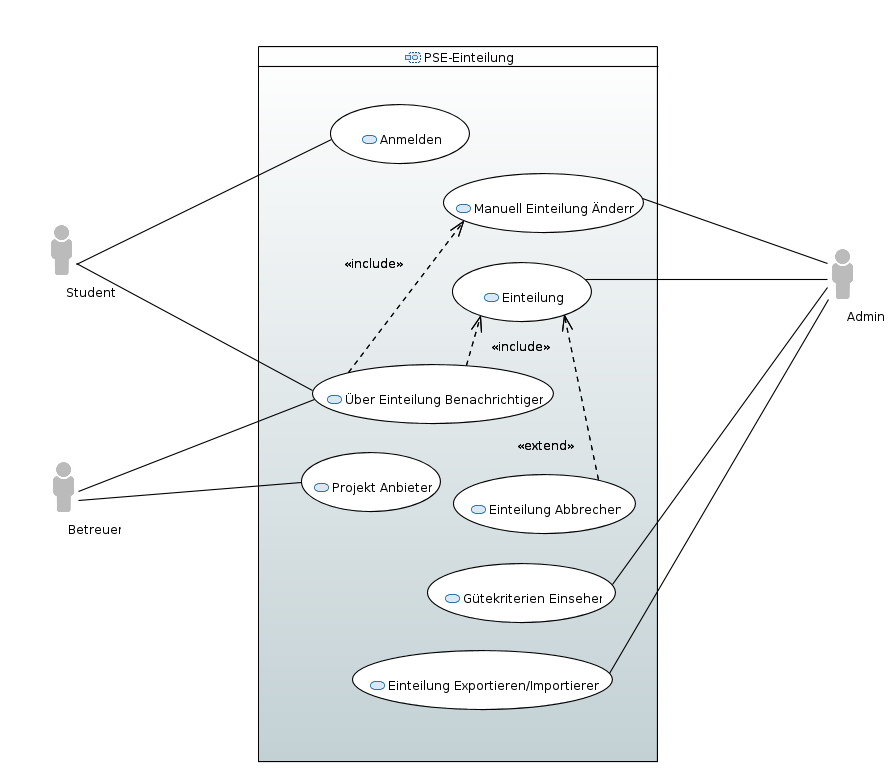
\includegraphics[width=\linewidth]{diagramme_pflichtenheft/UseCase_Diagram.PNG}
\captionof{figure}{Übersicht über die Anwendungsfälle}
\pagebreak

\subsubsection{Admin}
\begin{enumerate} [label=\swtLabel{A}, itemsep=2em]
	
	\item \label{UCadminInit}
	\begin{description}
		\item[Initialisierung des Produktes]
		\item[Ziel:] Das Produkt soll für den Einsatz vorbereitet werden
		\item[Vorbedingung:] -keine-
		\item[Nachbedingung:]
		\begin{description}[leftmargin=6em]
				\item[Erfolg] Das Produkt ist einsatzbereit und kann über das Webinterface bedient werden
				\item[Fehlschlag] Das Produkt ist nicht einsatzbereit und gibt
				eine aussagekräftige Fehlermeldung aus
		\end{description}

		\item[Beschreibung:]~
		\begin{enumerate} [label=\arabic*.]
			\item Der \gls{Admin} stellt auf dem Server Gurobi bereit %TODO Gurobi Glossar
			\item Er startet Web"= und Datenbankserver 
			\item Er startet das Produkt
		\end{enumerate}
		\item[Erweiterungen:] -keine-
		\item[Alternativen:]~
		\begin{enumerate}
			\item[2 a)] Kann entfallen, wenn Server bereits in Betrieb sind
		\end{enumerate}
		\item[Benötigte FA:] \ref{FAadminInit}
	\end{description}
	
	\item \label{UCadminAnmeldung}
    \begin{description}
    \item[Anmeldung des \gls{Admin}s]
    \item[Ziel:] \gls{Admin} wird angemeldet
  	\item[Vorbedingung:] -keine-
  	\item[Nachbedingung:]	\begin{description}[leftmargin=6em] \item[Erfolg]  Der \gls{Admin} ist angemeldet
  	\item[Fehlschlag] Der \gls{Admin} ist nicht angemeldet \end{description} 
  	\item[Beschreibung:]~
  	\begin{enumerate}
  	  \item[1.] \gls{Admin} öffnet die Website
  	  \item[2.] \gls{Admin} füllt das Formular mit \gls{Benutzername} und Passwort zum Anmelden aus und schickt
  	  dieses ab %TODO: Verweis auf Bild
  	  \item[3.] Sind die Anmeldedaten korrekt, so wird der \gls{Admin} zum
  	  \gls{Admin}bereich weitergeleitet
  	\end{enumerate}
  	\item[Erweiterungen:]  	
  	\item[Alternativen:]
	\begin{enumerate}
  	  \item[3a)] Wenn nicht, so erhält er eine Fehlermeldung
  	\end{enumerate}
  	\item[Benötigte FA:] \ref{FAadminAnmeldung}
  \end{description}
	
	\item \label{UCadminAnmeldezeit}
	\begin{description}
		\item[Setzten der frühestmöglichen Anmeldezeit]
		\item[Ziel:] Ein frühestmöglicher Zeitpunkt für die Anmeldung von \glspl{Studierender}n soll festgelegt werden
		\item[Vorbedingung:] \gls{Admin} ist angemeldet und im \gls{Admin}bereich der Webseite
		\item[Nachbedingung:]	\begin{description}[leftmargin=6em] \item[Erfolg]  Vor dem eingegeben Datum können sich
		\glspl{Studierender} nicht registrieren und einloggen
		\item[Fehlschlag] Registrieren und einloggen sind vor dem 
		Datum möglich \end{description}
		\item[Beschreibung:]~
		\begin{enumerate}[label=\arabic*.]
			\item Der \gls{Admin} klickt auf den Reiter \enquote{Einstellungen}
			\item Er befindet sich nun im Einstellungsbereich (\autoref{GUIeinstellungen})
			\item Er trägt in das Feld \enquote{Startzeit der Studentenanmeldung} ein
			Datum und eine Uhrzeit ein
		\end{enumerate}
		\item[Erweiterungen:] -keine-
		\item[Alternativen:] -keine-
		\item[Benötigte FA:] \ref{FAadminAnmeldezeit}
	\end{description}	
	
	\item \label{UCadminDeadline}
	\begin{description}
		\item[Setzten der \gls{Bewertung}sdeadline ]
		\item[Ziel:] Ein spätester Zeitpunkt für die Anmeldung von \glspl{Studierender}n soll festgelegt werden
		\item[Vorbedingung:] \gls{Admin} ist angemeldet und im \gls{Admin}bereich der Webseite
		\item[Nachbedingung:]	\begin{description}[leftmargin=6em] \item[Erfolg]  Nach dem eingegebenen Datum können sich keine \glspl{Studierender}n mehr anmelden
		\item[Fehlschlag] Anmelden ist weiter möglich \end{description}
		\item[Beschreibung:]~
		\begin{enumerate}[label=\arabic*.]
			\item Der \gls{Admin} klickt auf den Reiter \enquote{Einstellungen}
			\item Er befindet sich nun im Einstellungsbereich (\autoref{GUIeinstellungen})
			\item Er trägt in das Feld \enquote{Deadline für die Studenten\gls{Bewertung}en}
			ein Datum und eine Uhrzeit ein
		\end{enumerate}
		\item[Erweiterungen:] -keine-
		\item[Alternativen:] -keine-
		\item[Benötigte FA:] \ref{FAadminDeadline}
	\end{description}
	
  \item \label{UCadminProjektErstellenÄndern}
    \begin{description}
  	\item[Hinzufügen/Ändern eines \gls{Projekt}s]
  	\item[Ziel:] Einfügen/Änderung von \gls{Projekt}daten in der Datenbank
  	\item[Vorbedingung:] \gls{Admin} ist angemeldet und im \gls{Admin}bereich der Webseite
  	\item[Nachbedingung:]	\begin{description}[leftmargin=6em] \item[Erfolg]  Neue \gls{Projekt}daten sind eingetragen
  	\item[Fehlschlag] Neue \gls{Projekt}daten sind nicht eingetragen \end{description}
  	\item[Beschreibung:]~
  	\begin{enumerate} 
  	  \item[1.] \gls{Projekt}übersicht öffnen (\autoref{GUIprojUebersicht})
  	  \item[2.] Wenn das \gls{Projekt} schon existiert, so werden die \gls{Projekt}daten
  	  verglichen
  	  \item[3.] Ausfüllen der Eingabemaske (\autoref{GUIprojEdit})
  	  \item[4.] Stimmen die \gls{Projekt}daten nicht überein, so werden die betroffenen
  	  Daten angepasst
  	  \item[5.] Durch Abspeichern der Eingaben werden die Daten in der Datenbank
  	  geändert/hinzugefügt
  	\end{enumerate}
  	\item[Erweiterungen:] -keine-
  	\item[Alternativen:]~
  	\begin{enumerate}
  	  \item[2a)] Wenn nicht, dann wird das \gls{Projekt} neu angelegt
  	  \item[3a)] Falls doch, so ist dieser Anwendungsfall abgeschlossen
  	\end{enumerate} 
  	\item[Benötigte FA:] \ref{FAadminCreateProjekt}, \ref{FAadminProjektänderung}
  \end{description}
   
  
  \item \label{UCadminDeleteProjekt}
  \begin{description}
  \item[Löschen eines \glspl{Projekt}s]
  \item[Ziel:] Löschen eines \glspl{Projekt}s aus der Datenbank
  	\item[Vorbedingung:] \gls{Projekt} existiert bereits in der Datenbank und die
  	\glspl{Studierender}n konnten noch keine \gls{Bewertung} abgeben
  	\item[Nachbedingung:]	\begin{description}[leftmargin=6em] \item[Erfolg]  \gls{Projekt} ist aus der Datenbank entfernt
  	\item[Fehlschlag] \gls{Projekt} ist immer noch in der Datenbank \end{description}
  	\item[Beschreibung:]~
  	\begin{enumerate} 
  	  \item[1.] \gls{Projekt}übersicht öffnen (\autoref{GUIprojUebersicht})
  	  \item[2.] \gls{Projekt} aus Liste entfernen
  	  \item[3.] \gls{Projekt}daten werden aus der Datenbank entfernt
  	\end{enumerate}
  	\item[Erweiterungen:] -keine-
  	\item[Alternativen:] -keine-
  	\item[Benötigte FA:] \ref{FAadminDeleteProjekt}
  \end{description}
   
  
  \item \label{UCadminEinteilungStart}
  \begin{description}
  \item[\gls{Einteilung}]
  \item[Ziel:] Finden einer \gls{Einteilung} für eine bestimmte \gls{Einteilungskonfiguration}
  	\item[Vorbedingung:] Alle \glspl{Projekt} in der Datenbank sind vollständig
  	\item[Nachbedingung:]	\begin{description}[leftmargin=6em] \item[Erfolg]  Es wurde eine \gls{Einteilung} gefunden
  	\item[Fehlschlag] Es wurde keine \gls{Einteilung} gefunden \end{description}
  	\item[Beschreibung:]~
  	\begin{enumerate} 
  	  \item[1.] Einstellen der \gls{Einteilungskonfiguration}, nach denen eingeteilt werden
  	  soll(siehe \autoref{GUIeinteilung})
  	  \item[2.] Durch Klick auf \enquote{Zur Berechnung hinzufügen} wird die
  	  Berechnung gestartet
  	  \item[3.] Nach Abschluss der Berechnung wird das Ergebnis,  inklusive
  	  eingestellter \gls{Einteilungskonfiguration}, abgespeichert
  	\end{enumerate}
  	\item[Erweiterungen:] -keine-
  	\item[Alternativen:] ~
  	\begin{enumerate}
  	  \item[3a)] Hier ist auch ein frühzeitiger Abbruch durch den \gls{Admin}
  	  möglich. Dies wird im Ergebnis vermerkt.
  	 \end{enumerate}  
  	 \item[Benötigte FA:] \ref{FAadminParameter},
  	 \ref{FAadminEinteilungstart}, \ref{FAabbruch},
  	 \ref{FAeinteilungMussKriterien}, \ref{FAeinteilungWunschKriterien}
  \end{description}
   
  
  \item \label{UCadminEinteilungAuswahl}
  \begin{description}
  \item[Finale Auswahl der \gls{Einteilung}]
  \item[Ziel:] Finden der bestmöglichen \gls{Einteilung}
  	\item[Vorbedingung:] Es wurde mindestens eine \gls{Einteilung} berechnet
  	\item[Nachbedingung:]	\begin{description}[leftmargin=6em] \item[Erfolg]  Es wurde eine \gls{Einteilung} ausgewählt
  	\item[Fehlschlag] Es wurde keine \gls{Einteilung} ausgewählt \end{description}
  	\item[Beschreibung:]~
  	\begin{enumerate} 
  	  \item[1.] Öffnen der \gls{Einteilung}sübersicht (\autoref{GUIeinteilungErgeb})
  	  \item[2.] Auswahl des Reiters, der die zu veröffentliche \gls{Einteilung} enthält
  	  \item[3.] Durch Klick auf \enquote{\gls{Einteilung} veröffentlichen} wird diese
  	  \gls{Einteilung} final ausgewählt 
  	\end{enumerate}
  	\item[Erweiterungen:]~
  	\begin{enumerate}
  	  \item[nach 3)] \gls{Projektbetreuer} und \glspl{Studierender} werden per E"=Mail über die \gls{Einteilung} informiert
  	 \end{enumerate}
  	\item[Alternativen:] -keine-
  	\item[Benötigte FA:] \ref{FAadminAuswahl},
  	 \ref{FAadminBenachrichtigen}, \ref{FAadminUebersichtAlleEinteilungen} 
  \end{description}
  
  \item \label{UCadminCreateBetreuer}
  \begin{description}
  \item[Erstellen eines Betreueraccounts]
  \item[Ziel:] Hinzufügen eines \gls{Projektbetreuer} in das System
  	\item[Vorbedingung:] -keine-
  	\item[Nachbedingung:]	\begin{description}[leftmargin=6em] \item[Erfolg]  Der \gls{Projektbetreuer}account wurde erstellt
  	\item[Fehlschlag] Der \gls{Projektbetreuer}account wurde nicht erstellt \end{description}
  	\item[Beschreibung:]~
  	 \begin{enumerate} 
  	   \item[1.] Öffnen der Betreuerübersicht (\autoref{GUIprojLeiterUebersicht})
  	   \item[2.] Ausfüllen der einzeln abgetrennten Zeile  
  	   \item[3.] Durch Klick auf \enquote{Projektleiter hinzufügen} wird der neu
  	   angelegte \gls{Projektbetreuer} dem System hinzugefügt
  	 \end{enumerate} 
  	\item[Erweiterungen:]~
  	 \begin{enumerate}
  	   \item[4)] Der \gls{Projektbetreuer} erhält seine Zugangsdaten per E-Mail
  	 \end{enumerate}  
  \item[Alternativen:] -keine-
  \item[Benötigte FA:] \ref{FAadminCreateAccounts}
  \end{description}
  
  \item \label{UCadminLogout}
    \begin{description}
  	\item[Abmeldung]
  	\item[Ziel:] \gls{Admin} meldet sich ab
  	\item[Vorbedingung:] Der \gls{Admin} ist angemeldet und befindet sich im \gls{Admin}bereich
  	\item[Nachbedingung:]	\begin{description}[leftmargin=6em] \item[Erfolg]  Der \gls{Admin} ist abgemeldet und befindet sich auf der Startseite
  	\item[Fehlschlag] Der \gls{Admin} ist nicht abgemeldet \end{description}
  	\item[Beschreibung:]~
  	\begin{enumerate}
  	  \item[1.] \gls{Admin} ist im \gls{Admin}bereich der Webseite
      \item[2.] Klick auf \enquote{Ausloggen} in der Seitenleiste
      \item[3.] Die Startseite erscheint
  	\end{enumerate}
  	\item[Erweiterungen:] -keine-
  	\item[Alternativen:] -keine-
  	\item[Benötigte FA:] \ref{FAadminAbmeldung}
  \end{description}
  
  \item \label{UCadminEinteilungUebersicht}
    \begin{description}
  	\item[Anzeigen einer \gls{Einteilung}]
  	\item[Ziel:] Der \gls{Admin} bekommt Überblick über eine \gls{Einteilung}
  	\item[Vorbedingung:] Der \gls{Admin} ist angemeldet und befindet sich im \gls{Admin}bereich
  	\item[Nachbedingung:]	\begin{description}[leftmargin=6em] \item[Erfolg]  Der \gls{Admin} ist im Bereich
  	\enquote{\gls{Einteilung}sergebnisse}
  	\item[Fehlschlag] Der \gls{Admin} sieht keine \gls{Einteilung} \end{description}
  	\item[Beschreibung:]~
  	\begin{enumerate}
  	  \item[1.] \gls{Admin} ist im \gls{Admin}bereich der Webseite
      \item[2.] Klick auf \enquote{\gls{Einteilung}sergebnisse} in der Seitenleiste
      \item[3.] Der \gls{Admin} wählt eine \gls{Einteilung} aus
      \item[4.] Der \gls{Admin} sieht nun Details über die \gls{Einteilung}
  	\end{enumerate}
  	\item[Erweiterungen:] -keine-
  	\item[Alternativen:] -keine-
  	\item[Benötigte FA:] \ref{FAadminÜbersicht}
  \end{description}
  
  \item \label{UCadminSPOteilleistungAdd}
    \begin{description}
    \item[Hinzufügen einer wählbaren \gls{Teilleistung} zu einer
    \gls{SPO}]
    \item[Ziel:] Bei der Registrierung wird \glspl{Studierender}n eine weitere
    \glspl{Teilleistung} zur Auswahlahl angeboten
    \item[Vorbedingung:] Der \gls{Admin} ist angemeldet und befindet sich im \gls{Admin}bereich
    \item[Nachbedingung:]	\begin{description}[leftmargin=6em] \item[Erfolg]  Der \gls{Admin} ist im Bereich
    \enquote{Einstellungen} und hat eine neue \glspl{Teilleistung} zu einer \gls{SPO}
    hinzugefügt
    \item[Fehlschlag] Es wurde keine \glspl{Teilleistung} zu einer \gls{SPO} 
    hinzugefügt \end{description}
    \item[Beschreibung:]~
    \begin{enumerate}
      \item[1.] \gls{Admin} ist im \gls{Admin}bereich der Webseite
      \item[2.] Klick auf \enquote{Einstellungen} in der Seitenleiste
      \item[3.] Der \gls{Admin} wählt unter \enquote{SPOs} die \gls{SPO}, der er eine
      \glspl{Teilleistung} hinzufügen möchte
      \item[4.] Der \gls{Admin} gibt unter \enquote{SPOs} in das Textfeld
      neben \enquote{\glspl{Teilleistung} hinzufügen} den Namen der neuen \glspl{Teilleistung}
      ein
      \item[5.] Der \gls{Admin} klickt auf \enquote{\glspl{Teilleistung} hinzufügen}
      \item[6.] Die \glspl{Teilleistung} erscheint nun in der Aufzählung der
      \glspl{Teilleistung} als neuer Punkt
    \end{enumerate}
    \item[Erweiterungen:] -keine-
    \item[Alternativen:] -keine-
    \item[Benötigte FA:] \ref{FAadminSPOhinzufügen}
  \end{description}
  
  \item \label{UCadminSPOwelcheWerdeAngezeigt}
    \begin{description}
    \item[\glspl{SPO} wählen, die \glspl{Studierender}n angezeigt werden]
    \item[Ziel:] Nur die relevanten \glspl{SPO} werden bei der Registrierung von
    Studenten angezeigt
    \item[Vorbedingung:] Der \gls{Admin} ist angemeldet und befindet sich im \gls{Admin}bereich
    \item[Nachbedingung:]	\begin{description}[leftmargin=6em] \item[Erfolg]  Der \gls{Admin} ist im Bereich
    \enquote{Einstellungen} und nur noch die Relavanten \glspl{SPO} werden für
        \glspl{Studierender} angezeigt
    \item[Fehlschlag] Es gibt keine Veränderung \end{description}
    \item[Beschreibung:]~
    \begin{enumerate}
      \item[1.] Der \gls{Admin} ist im \gls{Admin}bereich der Webseite
      \item[2.] Klick auf \enquote{Einstellungen} in der Seitenleiste
      \item[3.] Der \gls{Admin} wählt unter \enquote{\glspl{SPO}} die \gls{SPO}, die er
      sichtbar oder unsichtbar machen möchte
      \item[4.] Der Adminstrator setzt oder entfernt das Häckchen bei
      \enquote{\gls{SPO} für \glspl{Studierender} anzeigen} %TODO richtige bezeichnung
      \item[5.] Falls es weitere \glspl{SPO} gibt, bei denen er die Sichtbarkeit
      verändern möchte, fängt er bei 3. erneut an  
    \end{enumerate}
    \item[Erweiterungen:] -keine-
    \item[Alternativen:] -keine-
    \item[Benötigte FA:] \ref{FAadminSPOAuswahl}
  \end{description}
  
  \item \label{UCadminSPOteilleistungRM}
    \begin{description}
    \item[Entfernen einer wählbaren \gls{Teilleistung} von einer
    \gls{SPO}]
    \item[Ziel:] Bei der Registrierung wird \glspl{Studierender}n die entfernte
    \glspl{Teilleistung} nicht mehr angezeigt
    \item[Vorbedingung:] Der \gls{Admin} ist angemeldet und befindet sich im
    \gls{Admin}bereich. Weiterhin gibt es eine \gls{SPO} mit einer wählbaren
    \glspl{Teilleistung}
    \item[Nachbedingung:]	\begin{description}[leftmargin=6em] \item[Erfolg]  Der \gls{Admin} ist im Bereich
    \enquote{Einstellungen} und die entfernte \glspl{Teilleistung} wird in der \gls{SPO}
    nicht mehr angezeigt
    \item[Fehlschlag] Es wurde keine \glspl{Teilleistung} entfernt \end{description}
    \item[Beschreibung:]~
    \begin{enumerate}
      \item[1.] \gls{Admin} ist im \gls{Admin}bereich der Webseite
      \item[2.] Klick auf \enquote{Einstellungen} in der Seitenleiste
       \item[3.] Der \gls{Admin} wählt unter \enquote{\glspl{SPO}} die \gls{SPO}, bei der er
       eine \glspl{Teilleistung} entfernen möchte
      \item[4.] Der \gls{Admin} setzt die Checkbox bei den \glspl{Teilleistung} die er
      entfernen möchte
      \item[5.] Der \gls{Admin} klickt \enquote{markierte \glspl{Teilleistung}
      löchen}
      \item[5.] Die \glspl{Teilleistung} erscheint nun nicht mehr in der Aufzählung der
      \glspl{Teilleistung} 
    \end{enumerate}
    \item[Erweiterungen:] -keine-
    \item[Alternativen:] -keine-
    \item[Benötigte FA:] \ref{FAadminSPOentfernen}
  \end{description}
  
    \item \label{UCadminImport}
    \begin{description}
    \item[Import von \gls{Einteilung}s"=, \gls{SPO}"= oder \glspl{Studierender}ndaten]
    \item[Ziel:] Testen mit Daten aus vergangenen Semestern oder die
    Wiederverwendung von \glspl{SPO}
    \item[Vorbedingung:] Der \gls{Admin} ist angemeldet und befindet sich im
    \gls{Admin}bereich
    \item[Nachbedingung:]	\begin{description}[leftmargin=6em] \item[Erfolg]  Der \gls{Admin} ist im \gls{Admin}bereich und die \gls{Einteilung}s"=, \gls{SPO}"= oder \glspl{Studierender}ndaten wurden in das aktive Semester importiert
    \item[Fehlschlag] Es wurden keine Daten importiert \end{description}
    \item[Beschreibung:]~
    \begin{enumerate}
      \item[1.] Der \gls{Admin} ist im \gls{Admin}bereich der Webseite
      \item[2.] Klick auf \enquote{Export/Import}
      in der Seitenleiste
       \item[3.] Der \gls{Admin} klickt auf den \enquote{Import}"=Knopf neben dem entsprechenden Datentyp, der importiert werden soll.
       \item[4.] Der \gls{Admin} kann in einem System"=Popup"=Fenster die Datei zum Importieren auswählen.
      \item[5.] Der \gls{Admin} wird über den Ausgang des Imports benachrichtigt.
    \end{enumerate}
    \item[Erweiterungen:] -keine-
    \item[Alternativen:] -keine-
    \item[Benötigte FA:] \ref{FAimport}
  \end{description}
  
      \item \label{UCadminExport}
    \begin{description}
    \item[Export von \gls{Einteilung}s"=, \gls{SPO}"= oder \glspl{Studierender}ndaten]
    \item[Ziel:] Export von \gls{Einteilung}s"=, \gls{SPO}"= oder \glspl{Studierender}ndaten zur Datensicherung
    \item[Vorbedingung:] Der \gls{Admin} ist angemeldet und befindet sich im
    \gls{Admin}bereich. Es müssen  \gls{Einteilung}s"=, \gls{SPO}"= oder \glspl{Studierender}ndaten existieren.
    \item[Nachbedingung:]	\begin{description}[leftmargin=6em] \item[Erfolg]  Der \gls{Admin} ist im \gls{Admin}bereich und die exportierten Daten wurden lokal auf dem Rechner des \gls{Admin}s gespeichert.
    \item[Fehlschlag] Es wurden keine Daten exportiert \end{description}
    \item[Beschreibung:]~
    \begin{enumerate}
      \item[1.] Der \gls{Admin} ist im \gls{Admin}bereich der Webseite
      \item[2.] Klick auf \enquote{Export/Import} in der Seitenleiste
       \item[3.] Der \gls{Admin} klickt auf den \enquote{Export}"=Knopf neben dem entsprechenden Datentyp, der exportiert werden soll.
       \item[4.] Der \gls{Admin} kann in einem System"=Popup"=Fenster den Speicherort der Exportdaten auswählen.
      \item[5.] Der \gls{Admin} wird über den Ausgang des Exports benachrichtigt.
    \end{enumerate}
    \item[Erweiterungen:] -keine-
    \item[Alternativen:] -keine-
    \item[Benötigte FA:] \ref{FAexport}
  \end{description}
  
      \item \label{UCadminImport2}
    \begin{description}
    \item[Import von Campus"=Management"=System"=Daten] %Kein \gls, wegen Bindestrichen! 
    \item[Ziel:] Datenabgleich von \glspl{Studierender}ndaten mit den \glspl{Studierender}ndaten aus dem \gls{CMS}
    \item[Vorbedingung:] Der \gls{Admin} ist angemeldet und befindet sich im
    \gls{Admin}bereich. Es müssen \glspl{Studierender}ndaten existieren.
    \item[Nachbedingung:]	\begin{description}[leftmargin=6em] \item[Erfolg]  Der \gls{Admin} ist im \gls{Admin}bereich und die \glspl{Studierender}ndaten aus dem \gls{CMS} wurden zu dem aktiven Semester hinzugefügt
    \item[Fehlschlag] Es wurden keine Daten importiert \end{description}
    \item[Beschreibung:]~
    \begin{enumerate}
      \item[1.] Der \gls{Admin} ist im \gls{Admin}bereich der Webseite
      \item[2.] Klick auf \enquote{Export/Import}
      in der Seitenleiste
       \item[3.] Der \gls{Admin} klickt auf den \enquote{Datei importieren}"=Knopf im \enquote{CMS Datenabgleich}"=Bereich.
       \item[4.] Der \gls{Admin} kann in einem System"=Popup"=Fenster die Datei zum Importieren auswählen.
      \item[5.] Der \gls{Admin} wird über den Ausgang des Imports benachrichtigt.
    \end{enumerate}
    \item[Erweiterungen:] -keine-
    \item[Alternativen:] -keine-
    \item[Benötigte FA:] \ref{FAimport2}
  \end{description}
  
    \item \label{UCadminKonfliktAnzeige}
    \begin{description}
    \item[Anzeige von Konflikten beim Import von Campus"=Management"=System"=Daten] (vgl. \ref{UCadminImport2})
    \item[Ziel:] Der \gls{Admin} sieht fehlende oder von \glspl{Studierender}n falsch angegebene \glspl{Teilleistung}.
    \item[Vorbedingung:] Der \gls{Admin} ist angemeldet und befindet sich im
    \gls{Admin}bereich. Es müssen \glspl{Studierender}ndaten existieren und ein Campus"=Management"=System"=Daten"=Import (vgl. \ref{UCadminImport2}) hat stattgefunden .
    \item[Nachbedingung:]	\begin{description}[leftmargin=6em] \item[Erfolg]  Der \gls{Admin} ist im \gls{Admin}bereich und sieht die tabellarisch aufgezählten Konflikte
    \item[Fehlschlag] ~ \end{description}
    \item[Beschreibung:]~
    \begin{enumerate}
      \item[1.] Der \gls{Admin} ist im \gls{Admin}bereich der Webseite
      \item[2.] Klick auf \enquote{Export/Import}
      in der Seitenleiste
       \item[3.] Der \gls{Admin} sieht die tabellarisch aufgezählten Konflikte im \enquote{CMS Datenabgleich}"=Bereich.
    \end{enumerate}
    \item[Erweiterungen:] -keine-
    \item[Alternativen:] -keine-
    \item[Benötigte FA:] \ref{FAkonfliktAnzeige}
  \end{description}
  
      \item \label{UCadminExport2}
    \begin{description}
    \item[Export von Campus"=Management"=System"=Daten]
    \item[Ziel:] Export von \glspl{Studierender}ndaten mit eingetragenen Noten zum automatischen Datenabgleich mit dem \gls{CMS}
    \item[Vorbedingung:] Der \gls{Admin} ist angemeldet und befindet sich im
    \gls{Admin}bereich. Es müssen \glspl{Studierender}ndaten existieren.
    \item[Nachbedingung:]	\begin{description}[leftmargin=6em] \item[Erfolg]  Der \gls{Admin} ist im \gls{Admin}bereich und die exportierten Daten wurden lokal auf dem Rechner des \gls{Admin}s gespeichert.
    \item[Fehlschlag] Es wurden keine Daten exportiert \end{description}
    \item[Beschreibung:]~
    \begin{enumerate}
      \item[1.] Der \gls{Admin} ist im \gls{Admin}bereich der Webseite
      \item[2.] Klick auf \enquote{Export/Import}
      in der Seitenleiste
       \item[3.] Der \gls{Admin} klickt auf den \enquote{Datei exportieren}"=Knopf im \enquote{CMS Datenabgleich}"=Bereich.
       \item[4.] Der \gls{Admin} kann in einem System"=Popup"=Fenster den Speicherort der Export"=Daten auswählen.
      \item[5.] Der \gls{Admin} wird über den Ausgang des Exports benachrichtigt.
    \end{enumerate}
    \item[Erweiterungen:] -keine-
    \item[Alternativen:] -keine-
    \item[Benötigte FA:] \ref{FAexport2}
  \end{description}
  
  \item \label{UCadminVergleichGuete}
    \begin{description}
  	\item[Vergleich von \glspl{Einteilung}]
  	\item[Ziel:] Vergleich von \glspl{Einteilung} anhand von \glspl{Guetekriterium}
  	\item[Vorbedingung:] Es wurde schon mindestens eine \gls{Einteilung} berechnet
  	\item[Nachbedingung:]	\begin{description}[leftmargin=6em] \item[Erfolg]  Der \gls{Admin} sieht einen Vergleich der
  	\glspl{Einteilung}
  	\item[Fehlschlag] Der \gls{Admin} sieht keinen Vergleich \end{description}
  	\item[Beschreibung:]~
  	\begin{enumerate}
  	  \item[1.] \gls{Admin} ist im \gls{Admin}bereich der Webseite
      \item[2.] Klick auf \enquote{\gls{Einteilung}sergebnisse} in der Seitenleiste
      \item[3.] Der \gls{Admin} wählt den Reiter \enquote{Vergleich} aus
      \item[4.] Der \gls{Admin} sieht nun einen Vergleich der \glspl{Einteilung}
  	\end{enumerate}
  	\item[Erweiterungen:] -keine-
  	\item[Alternativen:] -keine-
  	\item[Benötigte FA:] \ref{FAadminGüte}, \ref{FAguetekriterien} wobei die
  	berechneten \glspl{Guetekriterium} hier nur eingesehen werden können. Für die
  	Überprüfung muss eine \gls{Einteilung} exportiert und manuell nachgerechnet werden,
  	ob die \glspl{Guetekriterium} richtig berechnet wurden
  \end{description}
  
  \item \label{UCadminStapelverarbeitung}
    \begin{description}
  	\item[Nutzen der Stapelverarbeitung]
  	\item[Ziel:] Serielle Berechnung von \glspl{Einteilung}
  	\item[Vorbedingung:] Der \gls{Admin} befindet sich im Bereich
  	\enquote{\gls{Einteilung}}
  	\item[Nachbedingung:]	\begin{description}[leftmargin=6em] \item[Erfolg]  Alle gewünschten \glspl{Einteilung} werden berechnet
  	\item[Fehlschlag] Es werden nicht alle \glspl{Einteilung} berechnet \end{description}
  	\item[Beschreibung:]~
  	\begin{enumerate}
  	  \item[1.] \gls{Admin} ist im \gls{Admin}bereich der Webseite
      \item[2.] Klick auf \enquote{\gls{Einteilung}} in der Seitenleiste
      \item[3.] Der \gls{Admin} stellt die \gls{Einteilungskonfiguration} einer \gls{Einteilung} ein
      \item[4.] Klick auf \enquote{Zur Berechnung hinzufügen}
      \item[5.] Ist diese \gls{Einteilung} die erste in der Liste, so wird die
      Berechnung dieser direkt gestartet
      \item[6.] Wiederhole Schritte 3 und 4 bis alle gewünschten \glspl{Einteilung} in
      der Liste stehen
  	\end{enumerate}
  	\item[Erweiterungen:] -keine-
  	\item[Alternativen:] ~
  	\begin{enumerate}
  	  \item[5a)] Wenn nicht, so wird sie der Liste am Ende angehängt
  	\end{enumerate}  
  	\item[Benötigte FA:] \ref{FAadminStapel}, \ref{FAeinteilungStapel}
  \end{description}
  
  \item \label{UCadminCreateStudierender}
    \begin{description}
  	\item[Einen \glspl{Studierender}n zum System hinzufügen]
  	\item[Ziel:] Einen nicht registrierten \glspl{Studierender}n manuell zum System
  	hinzufügen
  	\item[Vorbedingung:] Der \gls{Admin} befindet sich im Bereich
  	\enquote{Studenten hinzufügen/löschen} und der \glspl{Studierender} ist noch nicht
  	registriert
  	\item[Nachbedingung:]	\begin{description}[leftmargin=6em] \item[Erfolg]  Der \glspl{Studierender} wurde dem System hinzugefügt
  	\item[Fehlschlag] Der \glspl{Studierender} wurde dem System nicht 
  	hinzugefügt \end{description}
  	\item[Beschreibung:]~
  	\begin{enumerate}
  	  \item[1.] \gls{Admin} ist im Bereich \enquote{Studenten
  	  hinzufügen/löschen}
      \item[2.] Ausfüllen der Maske \enquote{Student hinzufügen}
      \item[3.] Klick auf \enquote{Hinzufügen}
  	\end{enumerate}
  	\item[Erweiterungen:] -keine-
  	\item[Alternativen:] -keine-
  	\item[Benötigte FA:] \ref{FAadminAddStudToSystem}
  \end{description}
  
  \item \label{UCadminDeleteStudierender}
    \begin{description}
  	\item[Einen \glspl{Studierender}n aus dem System entfernen]
  	\item[Ziel:] Einen registrierten \glspl{Studierender}n aus dem System entfernen
  	\item[Vorbedingung:] Der \gls{Admin} befindet sich im Bereich
  	\enquote{Studenten hinzufügen/löschen}
  	\item[Nachbedingung:]	\begin{description}[leftmargin=6em] \item[Erfolg]  Der \glspl{Studierender} wurde aus dem System entfernt
  	\item[Fehlschlag] Der \glspl{Studierender} wurde nicht aus dem System 
  	entfernt \end{description}
  	\item[Beschreibung:]~
  	\begin{enumerate}
  	  \item[1.] \gls{Admin} ist im Bereich \enquote{Studenten
  	  hinzufügen/löschen}
      \item[2.] Ausfüllen der Maske \enquote{Student löschen}
      \item[3.] Klick auf \enquote{löschen}
  	\end{enumerate}
  	\item[Erweiterungen:] -keine-
  	\item[Alternativen:] -keine-
  	\item[Benötigte FA:] \ref{FAadminDeleteStudFromSystem}
  \end{description}
  
  \item \label{UCadminAddStudToTeam}
    \begin{description}
  	\item[Einen \glspl{Studierender}n zu einem \gls{Team} hinzufügen]
  	\item[Ziel:] Einen \glspl{Studierender}n manuell zu einem \gls{Team} hinzufügen
  	\item[Vorbedingung:] Der \gls{Admin} befindet sich im Bereich
  	\enquote{\gls{Einteilung}sergebnisse}
  	\item[Nachbedingung:]	\begin{description}[leftmargin=6em] \item[Erfolg]  Der \glspl{Studierender} wurde dem \gls{Team} hinzugefügt
  	\item[Fehlschlag] Der \glspl{Studierender} wurde dem \gls{Team} nicht 
  	hinzugefügt \end{description}
  	\item[Beschreibung:]~
  	\begin{enumerate}
  	  \item[1.] \gls{Admin} ist im Bereich \enquote{\gls{Einteilung}sergebnisse}
      \item[2.] Auswahl des \glspl{Studierender}n unter \enquote{Nicht zugeteilte
      Personen}
      \item[3.] Auswahl des \glspl{Team} im Drop"=Down"=Menü
      \item[4.] Klick auf \enquote{markierte Personen verschieben}
  	\end{enumerate}
  	\item[Erweiterungen:]~
  	\begin{enumerate}
  	  \item [zu 4.)] Überschreitet der \gls{Admin} die von ihm eingestellten
  	  Parameter (z.B. maximale \gls{Team}größe), so wird ihm eine Warnung angezeigt
  	\end{enumerate}  
  	\item[Alternativen:] -keine-
  	\item[Benötigte FA:] \ref{FAadminAddStudToTeam}, \ref{FAadminWarnung}
  \end{description}
  
  \item \label{UCadminRemoveStudFromTeam}
    \begin{description}
  	\item[Einen \glspl{Studierender}n aus einem \gls{Team} entfernen]
  	\item[Ziel:] Einen \glspl{Studierender}n manuell aus einem \gls{Team} entfernen
  	\item[Vorbedingung:] Der \gls{Admin} befindet sich im Bereich
  	\enquote{\gls{Einteilung}sergebnisse}
  	\item[Nachbedingung:]	\begin{description}[leftmargin=6em] \item[Erfolg]  Der \glspl{Studierender} wurde aus dem \gls{Team} entfernt
  	\item[Fehlschlag] Der \glspl{Studierender} wurde nicht aus dem \gls{Team} 
  	entfernt \end{description}
  	\item[Beschreibung:]~
  	\begin{enumerate}
  	  \item[1.] \gls{Admin} ist im Bereich \enquote{\gls{Einteilung}sergebnisse}
      \item[2.] Auswahl des \glspl{Studierender}n in der \gls{Team}übersicht
      \item[3.] im Drop"=Down"=Menü \enquote{Nicht zugeteilte
      Personen} auswählen
      \item[4.] Klick auf \enquote{markierte Personen verschieben}
  	\end{enumerate}
  	\item[Erweiterungen:]~
  	\begin{enumerate}
  	  \item [zu 4.)] Überschreitet der \gls{Admin} die von ihm eingestellten
  	  Parameter (z.B. minimale \gls{Team}größe), so wird ihm eine Warnung angezeigt
  	\end{enumerate}  
  	\item[Alternativen:] -keine-
  	\item[Benötigte FA:] \ref{FAadminRemoveStudFromTeam}, \ref{FAadminWarnung}
  \end{description}
  
  \item \label{UCadminSwapStudsBetweenTeams}
    \begin{description}
  	\item[\glspl{Studierender} zwischen zwei \glspl{Team} tauschen]
  	\item[Ziel:] Austauschen von zwei \glspl{Studierender}n
  	\item[Vorbedingung:] Der \gls{Admin} befindet sich im Bereich
  	\enquote{\gls{Einteilung}sergebnisse}
  	\item[Nachbedingung:]	\begin{description}[leftmargin=6em] \item[Erfolg]  Die \glspl{Studierender}n wurden getauscht
  	\item[Fehlschlag] Die \glspl{Studierender}n sind immer noch in ihren 
  	alten \glspl{Team} \end{description}
  	\item[Beschreibung:]~
  	\begin{enumerate}
  	  \item[1.] \gls{Admin} ist im Bereich \enquote{\gls{Einteilung}sergebnisse}
      \item[2.] Auswahl der beiden \glspl{Studierender}n in der \gls{Team}übersicht
      \item[3.] Klick auf \enquote{markierte Personen tauschen}
  	\end{enumerate}
  	\item[Erweiterungen:]~
  	\begin{enumerate}
  	  \item [zu 4.)] Überschreitet der \gls{Admin} die von ihm eingestellten
  	  Parameter (z.B. zerrissene \glspl{Lerngruppe}), so wird ihm eine Warnung angezeigt
  	\end{enumerate}  
  	\item[Alternativen:] -keine-
  	\item[Benötigte FA:] \ref{FAadminMoveStudsBetweenTeams}, \ref{FAadminWarnung}
  \end{description}
  
\end{enumerate}  
\subsubsection{Studierender}

\begin{enumerate}[label=\swtLabel{S}, itemsep=2em]
	\item \label{UCstudReg}
    \begin{description}
  	\item[Registrierung eines \glspl{Studierender}n]
  	\item[Ziel:] Speichern der \glspl{Studierender}ndaten in der Datenbank
  	\item[Vorbedingung:] Registrierung wurde freigeschaltet
  	\item[Nachbedingung:]	\begin{description}[leftmargin=6em] \item[Erfolg]  Erfolgreiche Registrierung des \glspl{Studierender}n
  	\item[Fehlschlag] \gls{Studierender} ist weiterhin nicht 
  	registriert \end{description}
  	\item[Beschreibung:]~
  	\begin{enumerate}
  	  \item[1.] Öffnen der Internetseite
      \item[2.] Klick auf Registrieren
      \item[3.] Ausfüllen der Registrierungsmaske %TODO Verweis auf Bild
      \item[4.] Abschicken der Daten
      \item[5.] Existiert der registrierte Account noch nicht, so wird der
      \glspl{Studierender} der Datenbank hinzugefügt
  	\end{enumerate}
  	\item[Erweiterungen:]~
  	\begin{enumerate}
  	  \item[zu 3)] Statt der Registrierungsmaske wird hier der \gls{SCC-Account}
  	  verwendet
  	  \item[nach 4)] Dem \glspl{Studierender}n wird nach dem Abschicken seiner Daten eine
  	  \\
  	  Verifikations-Email gesendet. (siehe \testRef{UCstudVerifikationEmail})
  	 \end{enumerate} 
  	\item[Alternativen:]~
  	\begin{enumerate}
  	  \item[5a)] Wenn doch, so wird kein weiterer Eintrag hinzugefügt, sondern
  	  die zweite Registrierung abgebrochen
  	\end{enumerate} 
  	\item[Benötigte FA:] \ref{FAregistrierung}, \ref{FAstudUanmeldung}
  \end{description}
%   
  
  \item \label{UCstudVerifikationEmail}
    \begin{description}
    \item[Verifikation der E"=Mail"=Adresse]
    \item[Ziel:] Verifikation der E"=Mail"=Adresse
    \item[Vorbedingung:] \gls{Studierender} muss sich registriert haben und seine
    E"=Mail"=Adresse korrekt angegeben haben.
    \item[Nachbedingung:]	\begin{description}[leftmargin=6em] \item[Erfolg]  \gls{Studierender} kann sich nun Anmelden und hat
    Zugriff auf den \glspl{Studierender}nbereich
    \item[Fehlschlag] \gls{Studierender} kann sich nicht mit seinem Account anmelden \end{description}
    \item[Beschreibung:]~
    \begin{enumerate}
      \item[1.] E-Mails über Drittsoftware abrufen.
      \item[2.] Klick auf den Verifikations-Link in der E"=Mail.      
    \end{enumerate}
    \item[Erweiterungen:] -keine-
    \item[Alternativen:] -keine-
    \item[Benötigte FA:] \ref{FAemailverifikation}
      \end{description}
  
  \item \label{UCstudAnmeldung}
    \begin{description}
    \item[Anmeldung eines \glspl{Studierender}n]
    \item[Ziel:] \gls{Studierender} wird angemeldet und kann seine \gls{Bewertung} ändern
  	\item[Vorbedingung:] Der \glspl{Studierender} hat sich vorher registriert
  	\item[Nachbedingung:]	\begin{description}[leftmargin=6em] \item[Erfolg]  Der \glspl{Studierender} ist angemeldet
  	\item[Fehlschlag] Der \glspl{Studierender} ist nicht angemeldet \end{description}
  	\item[Beschreibung:]~
  	\begin{enumerate}
  	  \item[1.] \gls{Studierender} öffnet die Website
  	  \item[2.] \gls{Studierender} füllt das Formular zum Anmelden aus und schickt
  	  dieses ab %TODO: Verweis auf Bild
  	  \item[3.] Sind die Anmeldedaten korrekt, so wird der \glspl{Studierender} zum
  	  \glspl{Studierender}nbereich weitergeleitet
  	\end{enumerate}
  	\item[Erweiterungen:]
  	\begin{enumerate}
  	  \item[2)] Kein Formular, sondern Anmeldung über \gls{SCC-Account}
  	\end{enumerate}    	
  	\item[Alternativen:]
	\begin{enumerate}
  	  \item[3a)] Wenn nicht, so erhält er eine Fehlermeldung
  	\end{enumerate}
  	\item[Benötigte FA:] \ref{FAStudanmeldung}, \ref{FAstudUanmeldung}
  \end{description}
   
  
  \item \label{UCstudCrealernG}
  \begin{description}
  \item[\gls{Studierender} erstellt \gls{Lerngruppe}]
  \item[Ziel:] Eine neue \gls{Lerngruppe} ist in der Datenbank vermerkt und der
  Ersteller ist erstes Mitglied dieser
  	\item[Vorbedingung:] \gls{Studierender} ist angemeldet und befindet sich auf der
  	Website im \glspl{Studierender}nportal
  	\item[Nachbedingung:]	\begin{description}[leftmargin=6em] \item[Erfolg]  Die \gls{Lerngruppe} wurde erfolgreich erstellt
  	\item[Fehlschlag] Die \gls{Lerngruppe} wurde nicht erstellt \end{description}
  	\item[Beschreibung:]~
  	\begin{enumerate}
  	  \item[1.] \gls{Studierender} gibt Name und Passwort in das Formular zum Erstellen
  	  einer \gls{Lerngruppe} ein und schickt dieses ab %TODO: Verweis einfügen
  	  \item[2.] Wenn noch keine \gls{Lerngruppe} mit diesem Namen existiert, so
  	  wird die \gls{Lerngruppe} in der Datenbank angelegt und der Ersteller wird
  	  erstes Mitglied
  	\end{enumerate}
  	\item[Erweiterungen:] -keine-
  	\item[Alternativen:] ~
  	\begin{enumerate}
  	  \item[2a)] Eine \gls{Lerngruppe} mit diesem Namen existiert schon. Dann
  	  wird keine weitere \gls{Lerngruppe} angelegt und dem \glspl{Studierender}n wird
  	  mitgeteilt, dass er den Namen der \gls{Lerngruppe} verändern soll
  	 \end{enumerate}
  	 \item[Benötigte FA:] \ref{FAcreatelerng}
  \end{description}
   
  
  \item \label{UCstudJoinLernG}
  \begin{description}
  \item[\gls{Studierender} tritt \gls{Lerngruppe} bei]
  \item[Ziel:] \gls{Studierender} ist Mitglied einer \gls{Lerngruppe}
  	\item[Vorbedingung:] \gls{Studierender} ist angemeldet und befindet sich auf der
  	Webseite im \glspl{Studierender}nberiech
  	\item[Nachbedingung:]	\begin{description}[leftmargin=6em] \item[Erfolg]  Der \glspl{Studierender} ist Mitglied der
  	\gls{Lerngruppe}
  	\item[Fehlschlag] Der \glspl{Studierender} ist nicht Mitglied der 
  	\gls{Lerngruppe} \end{description}
  	\item[Beschreibung:]~
  	\begin{enumerate}
  	  \item[1.] Der \glspl{Studierender} gibt die Anmeldedaten der \gls{Lerngruppe} in das
  	  passende Formular ein und schickt dieses ab %TODO: Verweis
  	  \item[2.] Existiert die angegebene \gls{Lerngruppe}, so wird die
  	  Mitgliederliste der \gls{Lerngruppe} um den \glspl{Studierender}n erweitert
  	\end{enumerate}
  	\item[Erweiterungen:]~
  	\begin{enumerate}
  	  \item[2a)] Ist die \gls{Lerngruppe} schon vollständig, so wird der
  	  \glspl{Studierender} nicht der Gruppe zugewiesen
  	  \item[3)] Ist der \glspl{Studierender} nicht der \gls{Lerngruppe} zugewiesen worden,
  	  so werden die zuletzt gespeicherten \gls{Bewertung} verwendet
  	  \item[4)] Die gesamte \glspl{Lerngruppe} wird per E-Mail informiert
  	 \end{enumerate}
  	\item[Alternativen:] ~
  	\begin{enumerate}
  	  \item[2a)] Existiert keine solche Gruppe, so schlägt der Beitritt fehl und
  	  der \glspl{Studierender} ist kein Mitglied der \gls{Lerngruppe}
  	 \end{enumerate}
  	 \item[Benötigte FA:] \ref{FAjoinLerng}
  \end{description}
  
   \item \label{UCstudUebersichtLernG}
  \begin{description}
  \item[Übersicht über \gls{Lerngruppe}]
  \item[Ziel:] \gls{Studierender} kann sehen wer in seiner \gls{Lerngruppe} ist
  	\item[Vorbedingung:] \gls{Studierender} ist angemeldet und befindet sich auf der
  	Webseite im \glspl{Studierender}nbereich. Weiterhin ist der \glspl{Studierender} Mitglied einer
  	\gls{Lerngruppe}
  	\item[Nachbedingung:]	\begin{description}[leftmargin=6em] \item[Erfolg]  \gls{Studierender} befindet sich nun in der
  	\glspl{Lerngruppe}übersicht
  	\item[Fehlschlag] Der \glspl{Studierender} ist nicht in der 
  	\glspl{Lerngruppe}übersicht \end{description}
  	\item[Beschreibung:]~
  	\begin{enumerate}
  	  \item[1.] Der \glspl{Studierender} klickt auf \gls{Lerngruppe} %TODO Verweis
    \end{enumerate}
  	\item[Erweiterungen:] -keine-
  	\item[Alternativen:] -keine-  	
  	\item[Benötigte FA:] \ref{FAcheckLerng}
  \end{description}
  
     \item \label{UCstudEinsichtEinteilung}
  \begin{description}
  \item[Einsicht der \gls{Einteilung}sergebnisse]
  \item[Ziel:] \gls{Studierender} kann sehen welchem \gls{Projekt} er
  zugeteilt wurde
  	\item[Vorbedingung:] \gls{Studierender} ist angemeldet und befindet sich auf der
  	Webseite im \glspl{Studierender}nbereich. 
  	\item[Nachbedingung:]	\begin{description}[leftmargin=6em] \item[Erfolg]  \gls{Studierender} befindet sich in der Maske
  	\gls{Einteilung}sergebnisse. %TODO verweis
  	Falls der \gls{Admin} die \gls{Einteilung}sergebnisse bereits veröffentlicht hat,
  	kann er sehen, welchem \gls{Projekt} er zugeteilt wurde. Sonst sieht er, dass
  	die \gls{Einteilung} noch im Gange ist %TODO Gehört der Abschnitt hier rein?
  	\item[Fehlschlag] Der \glspl{Studierender} ist nicht in der 
  	Maske \gls{Einteilung}sergebnisse \end{description}
  	\item[Beschreibung:]~
  	\begin{enumerate}
  	  \item[1.] Der \glspl{Studierender} klickt auf \gls{Einteilung}sergebnisse
 
  	\end{enumerate}
  	\item[Erweiterungen:] -keine-

  	\item[Alternativen:] -keine-
  	
  	 \item[Benötigte FA:] \ref{FAStudeinsicht}
  \end{description}
  
    \item \label{UCstudProjektbeschreibung}
  \begin{description}
  \item[Anzeigen der \gls{Projekt}beschreibung in \gls{Bewertung}smaske]
  \item[Ziel:] \gls{Studierender} kann sich während der \gls{Einteilung} die Beschreibung
  der zu bewertenden \glspl{Projekt} nochmals ansehen
  	\item[Vorbedingung:] \gls{Studierender} ist angemeldet und befindet sich in der
  	Projekt\gls{Bewertung}smaske %TODO verweis
  	
  	\item[Nachbedingung:]	\begin{description}[leftmargin=6em] \item[Erfolg]  \gls{Studierender} kann die \gls{Projekt}beschreibung als
  	\enquote{Overlay} sehen %TODO wirklich als overlay? wie sieht der Studierend
  	%die beschreibunmg e
  	
  	\item[Fehlschlag] Der \glspl{Studierender} kann die 
  	Projektbeschreibung nicht sehen \end{description}
  	\item[Beschreibung:]~
  	\begin{enumerate}
  	  \item[1.] Der \glspl{Studierender} fährt mit seiner Maus über den \gls{Projekt}namen
 
  	\end{enumerate}
  	\item[Erweiterungen:] -keine-

  	\item[Alternativen:] -keine-

  	 \item[Benötigte FA:] \ref{FAbeschreibung-Bewertung}
  \end{description}
  
      \item \label{UCstudLeaveLernG}
  \begin{description}
  \item[Austritt aus einer \gls{Lerngruppe}]
  \item[Ziel:] \gls{Studierender} möchte aus einer \gls{Lerngruppe} austreten
  	\item[Vorbedingung:] \gls{Studierender} ist angemeldet und befindet sich auf der
  	Webseite im \glspl{Studierender}nbereich. Weiterhin ist er Mitglied
  	einer \gls{Lerngruppe}
  	%TODO verweis
  	
  	\item[Nachbedingung:]	\begin{description}[leftmargin=6em] \item[Erfolg]  \gls{Studierender} ist kein Mitglied der
  	\gls{Lerngruppe} mehr
  	
  	\item[Fehlschlag] \gls{Studierender} ist immer noch Mitglied der 
  	\gls{Lerngruppe} \end{description}
  	\item[Beschreibung:]~
  	\begin{enumerate}
  	  \item[1.] Der \glspl{Studierender} klickt auf \gls{Lerngruppe}. Nun befindet er sich
  	  in der \enquote{\gls{Lerngruppe}}-Maske %TODO verweis
  	  \item[2.] Der \glspl{Studierender} klickt auf \enquote{Austreten}
 
  	\end{enumerate}
  	\item[Erweiterungen:] -keine-

  	\item[Alternativen:] -keine-

  	 \item[Benötigte FA:] \ref{FAlergAustritt}
  \end{description}
%   
  
  \item \label{UCstudBewertung}
  \begin{description}
  \item[\gls{Studierender} bewertet \glspl{Projekt}]
  \item[Ziel:] Der \glspl{Studierender} hat eine \gls{Bewertung} abgegeben
  	\item[Vorbedingung:] Der \glspl{Studierender} ist angemeldet und im \glspl{Studierender}nportal der
  	Website
  	\item[Nachbedingung:]	\begin{description}[leftmargin=6em] \item[Erfolg]  Die \gls{Bewertung} wurde gespeichert
  	\item[Fehlschlag] Die \gls{Bewertung} wurde nicht gespeichert \end{description}
  	\item[Beschreibung:]~
  	 \begin{enumerate}
  	   \item[1.] Der \glspl{Studierender} füllt die \gls{Bewertung}smaske aus %TODO: Verweis
  	   \item[2.] Der \glspl{Studierender} speichert die \gls{Bewertung} ab
  	   \item[3.] Ist der \glspl{Studierender} Mitglied einer \gls{Lerngruppe}, so gilt die
  	   \gls{Bewertung} gleichzeitig auch für alle anderen Mitglieder
  	 \end{enumerate}
  	\item[Erweiterungen:] -keine-
  	\item[Alternativen:] ~
  	\begin{enumerate}
  	  \item[3a)] Wenn nicht, so gilt sie nur für den \glspl{Studierender}n
  	 \end{enumerate}
  	\item[Benötigte FA:] \ref{FAbewertung}, \ref{FAbewertung2}
  \end{description}

 
  \item \label{UCstudNewPasswort}
    \begin{description}
  	\item[Passwort vergessen]
  	\item[Ziel:] Erhalten eines neuen Passworts
  	\item[Vorbedingung:] Der \glspl{Studierender} hat schon einen Account
  	\item[Nachbedingung:]	\begin{description}[leftmargin=6em] \item[Erfolg]  Der \glspl{Studierender} erhält eine E-Mail mit einem
  	neuen Passwort
  	\item[Fehlschlag] Der \glspl{Studierender} erhält keine E-Mail \end{description}
  	\item[Beschreibung:]~
  	\begin{enumerate}
  	  \item[1.] Öffnen der Internetseite
      \item[2.] Klick auf \enquote{Passwort vergessen}
      \item[3.] Eingabe der E"=Mail"=Adresse
      \item[4.] Der \glspl{Studierender} erhält eine E"=Mail mit seinem neuen Passwort
  	\end{enumerate}
  	\item[Erweiterungen:] -keine-
  	\item[Alternativen:] -keine-
  	\item[Benötigte FA:] \ref{FApasswortvergessen}
  \end{description}
  
  \item \label{UCstudLogout}
    \begin{description}
  	\item[Abmeldung]
  	\item[Ziel:] Student meldet sich ab
  	\item[Vorbedingung:] Der \glspl{Studierender} ist angemeldet und befindet sich im \glspl{Studierender}nbereich
  	\item[Nachbedingung:]	\begin{description}[leftmargin=6em] \item[Erfolg]  Der \glspl{Studierender} ist abgemeldet und befindet sich auf der Startseite
  	\item[Fehlschlag] Der \glspl{Studierender} ist nicht abgemeldet \end{description}
  	\item[Beschreibung:]~
  	\begin{enumerate}
  	  \item[1.] \gls{Studierender} ist im \glspl{Studierender}nbereich der Webseite
      \item[2.] Klick auf \enquote{Ausloggen} in der Seitenleiste
      \item[3.] Die Startseite erscheint
  	\end{enumerate}
  	\item[Erweiterungen:] -keine-
  	\item[Alternativen:] -keine-
  	\item[Benötigte FA:] \ref{FAStudabmeldung}
  \end{description}
   
\end{enumerate}

\subsubsection{Betreuer}
\begin{enumerate} [label=\swtLabel{B}, itemsep=2em]
  \item \label{UCbetreuerAnmeldung}
	 \begin{description}
		\item[\gls{Projektbetreuer} meldet sich an]
  		\item[Ziel:] Anmeldung des \gls{Projektbetreuer}s
  		\item[Vorbedingung:] Konto des \gls{Projektbetreuer}s wurde angelegt
  		\item[Nachbedingung:]	\begin{description}[leftmargin=6em] \item[Erfolg]  \gls{Projektbetreuer} ist angemeldet
  		\item[Fehlschlag] \gls{Projektbetreuer} ist nicht angemeldet \end{description}
  		\item[Beschreibung]~
  		\begin{enumerate}
  			\item[1.] Der \gls{Projektbetreuer} gibt seine Zugangsdaten ein
  			\item[2.] Wenn die Anmeldedaten korrekt sind, wird er auf den
  			Betreuerbereich weitergeleitet
  		\end{enumerate}
  		\item[Erweiterungen:] -keine-
  		\item[Alternativen:] ~
  		\begin{enumerate}
  		  \item[2a)] Wenn nicht, erhält er eine Fehlermeldung
  		\end{enumerate}  
  		\item[Benötigte FA:] \ref{FAbetreuerAnmeldung}
  	\end{description}
   
  
  \item \label{UCbetreuerThemaErstellenÄndern}
	\begin{description}
  		\item[\gls{Projekt} erstellen/ändern]
  		\item[Ziel:] Eröffnung/Änderung eines \glspl{Projekt}s
  		\item[Vorbedingung:] -keine-
  		\item[Nachbedingung:]	\begin{description}[leftmargin=6em] \item[Erfolg]  \gls{Projekt}daten sind im System eingetragen
  		\item[Fehlschlag] \gls{Projekt}daten sind nicht im System 
  		eingetragen \end{description}
  		\item[Beschreibung:]~
  	\begin{enumerate}
  	  \item[1.] \gls{Projektbetreuer} befindet sich auf der Website mit den \gls{Projekt}
  	  \item[2.] Existiert das \gls{Projekt} schon, so wählt der \gls{Projektbetreuer} dieses aus
  	  \item[3.] \gls{Projektbetreuer} füllt die Eingabemaske aus
  	  \item[4.] \gls{Projektbetreuer} speichert die neuen Daten ab
  	\end{enumerate}
  	\item[Erweiterungen:] -keine-
  	\item[Alternativen:]~
  	\begin{enumerate}
  	  \item[2a)] Wenn nicht, so fügt er ein neues hinzu
  	\end{enumerate}  
  	\item[Benötigte FA:] \ref{FAbetreuerAddProjekt}, \ref{FAbetreuerChangeProjekt}
  \end{description}

 
  \item \label{UCbetreuerJoinProjekt}
	\begin{description}
  		\item[\gls{Projektbetreuer} werden]
  		\item[Ziel:] \gls{Projektbetreuer} eines bestimmten \glspl{Projekt}s werden
  		\item[Vorbedingung:] Man ist noch nicht \gls{Projektbetreuer} des ausgewählten \glspl{Projekt}s
  		\item[Nachbedingung:]	\begin{description}[leftmargin=6em] \item[Erfolg]  Erfolgreich \gls{Projektbetreuer} des ausgewählten
  		\glspl{Projekt}s geworden
  		\item[Fehlschlag] Man ist nicht \gls{Projektbetreuer} des \glspl{Projekt}s \end{description}
  		\item[Beschreibung:]~
  	\begin{enumerate} 
  	  \item[1.] \gls{Projektbetreuer} befindet sich auf der Website mit den \glspl{Projekt}n
  	  \item[2.] \gls{Projektbetreuer} wählt das \gls{Projekt} aus, welches er betreuen möchte
  	  \item[3.] \gls{Projektbetreuer} tritt dem \gls{Projekt} bei
  	\end{enumerate}
  	\item[Erweiterungen:] -keine-
  	\item[Alternativen:] -keine-
  	\item[Benötigte FA:] \ref{FAbetreuerJoinProjekt}
  \end{description}
  
  
  \item \label{UCbetreuerEinsichtEinteilungProjekt}
  \begin{description}
  	\item[Einsicht der \gls{Einteilung}sergebnisse und zusätzlicher Informationen]
  	\item[Ziel:] Der \gls{Projektbetreuer} kann sehen, wer zu seinen \glspl{Projekt}n zugeteilt wurde und erhält weitere Informationen
  	\item[Vorbedingung:] \gls{Projektbetreuer} ist angemeldet und befindet sich auf der
  	Webseite im Betreuerbereich  %TODO noch kein GUI entwurf
  	\item[Nachbedingung:]	\begin{description}[leftmargin=6em] \item[Erfolg]  \gls{Projektbetreuer} befindet sich in der Maske
  	\gls{Einteilung}sergebnisse. %TODO verweis
  	Falls der \gls{Admin} die \gls{Einteilung}sergebnisse bereits veröffentlicht hat, kann er
  	sehen, wer seinen \glspl{Projekt}n zugeteilt wurde. Sonst sieht er, dass die \gls{Einteilung}
  	noch im Gange ist
  	\item[Fehlschlag] Der \gls{Projektbetreuer} ist nicht in der
  	Maske \gls{Einteilung}sergebnisse \end{description}
  	\item[Beschreibung:]~
  	\begin{enumerate}
  		\item[1.] Der \gls{Projektbetreuer} klickt auf \enquote{\gls{Einteilung}sergebnisse} 
		\item[2.] Der \gls{Projektbetreuer} sieht, welche \glspl{Studierender} in welchen \glspl{Team} seinem \gls{Projekt} zugeordnet wurden. Zusätzlich erhält er die Information, ob \glspl{Studierender} sich im CMS schon zum \gls{PSE} und \gls{TSE} angemeldet haben und ob noch \glspl{Teilleistung} offen sind.
  	\end{enumerate}
  	\item[Erweiterungen:] -keine-
  	
  	\item[Alternativen:] -keine-
  	
  	\item[Benötigte FA:] \ref{FAbetreuerEinsichtEinteilung}, \ref{FAbetreuerEinsichtNachpruefung}, \ref{FAbetreuerEinsichtTSE}
  \end{description}
   
  
  \item \label{UCbetreuerLeaveProjekt}
	\begin{description}
  		\item[\gls{Projekt} verlassen]
  		\item[Ziel:] Ein \gls{Projekt} nicht mehr betreuen
  		\item[Vorbedingung:] Man ist \gls{Projektbetreuer} eines \glspl{Projekt}s, in dem noch mindestens
  		ein anderer \gls{Projektbetreuer} ist.
  		\item[Nachbedingung:]	\begin{description}[leftmargin=6em] \item[Erfolg]  Man betreut das \gls{Projekt} nicht länger
  		\item[Fehlschlag] Man ist immer noch \gls{Projektbetreuer} des \glspl{Projekt}s \end{description}
  		\item[Beschreibung:]~
  	\begin{enumerate} 
  	  \item[1.] \gls{Projektbetreuer} befindet sich auf der Website mit den \glspl{Projekt}n, die
  	  er betreut.
  	  \item[2.] \gls{Projektbetreuer} wählt das \gls{Projekt} aus, welches er verlassen möchte.
  	  \item[3.] \gls{Projektbetreuer} verlässt das \gls{Projekt}.
  	\end{enumerate}
  	\item[Erweiterungen:] -keine-
  	\item[Alternativen:] -keine-
  	\item[Benötigte FA:] \ref{FAbetreuerLeaveprojekt}
  \end{description}
   
  
  \item \label{UCbetreuerNoteneintragung}
    \begin{description}
  	\item[Noten für \gls{Team} eintragen]
  	\item[Ziel:] Speichern der Noten in der Datenbank
  	\item[Vorbedingung:] \gls{Team} hat \glspl{Studierender}n als Teilnehmer
  	\item[Nachbedingung:]	\begin{description}[leftmargin=6em] \item[Erfolg]  Eintragung/Änderung der Noten
  	\item[Fehlschlag] Notenänderung wird verworfen \end{description}
  	\item[Beschreibung:]~
  	\begin{enumerate} 
  	  \item[1.] \gls{Projektbetreuer} befindet sich auf der Website mit der Notenübersicht
  	  \item[2.] \gls{Projektbetreuer} trägt neue Noten für einen \glspl{Studierender}n ein oder
  	  ändert bestehende Noten
  	\end{enumerate}
  	\item[Erweiterungen:] -keine-
  	\item[Alternativen] -keine-
  	\item[Benötigte FA:] \ref{FAbetreuerNoten}
  \end{description}
  
  \item \label{UCbetreuerLogout}
    \begin{description}
  	\item[Abmeldung]
  	\item[Ziel:] \gls{Projektbetreuer} meldet sich ab
  	\item[Vorbedingung:] Der \gls{Projektbetreuer} ist angemeldet und befindet sich im Betreuerbereich
  	\item[Nachbedingung:]	\begin{description}[leftmargin=6em] \item[Erfolg]  Der \gls{Projektbetreuer} ist abgemeldet und befindet sich auf der Startseite
  	\item[Fehlschlag] Der \gls{Projektbetreuer} ist nicht abgemeldet \end{description}
  	\item[Beschreibung:]~
  	\begin{enumerate}
  	  \item[1.] \gls{Projektbetreuer} ist im Betreuerbereich der Webseite
      \item[2.] Klick auf \enquote{Ausloggen} in der Seitenleiste
      \item[3.] Die Startseite erscheint
  	\end{enumerate}
  	\item[Erweiterungen:] -keine-
  	\item[Alternativen:] -keine-
  	\item[Benötigte FA:] \ref{FAbetreuerAbmeldung}
  \end{description}
   
\end{enumerate}



\subsection{Objektmodelle}

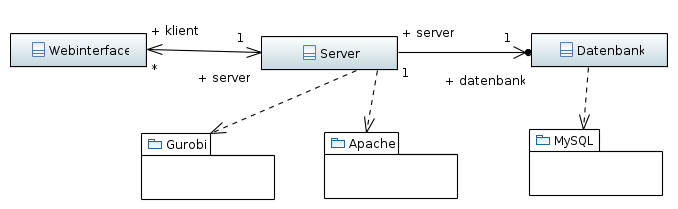
\includegraphics[width=\linewidth]{diagramme_pflichtenheft/ClassDiagram.PNG}
\captionof{figure}{Schematischer Aufbau des Produkts}

%TODO Brauchen wir das? \subsection{Dynamische Modelle}

\subsection{Benutzerschnittstelle}
\begin{enumerate}
  \item Es ist eine Benutzung rein über ein Web-Interface vorgesehen
  \item Es sind drei Bereiche zu unterscheiden:
        \begin{itemize}
          \item der \glspl{Studierender}nbereich
          \item der Betreuerbereich
          \item der \gls{Admin}bereich
        \end{itemize}
  \item Die jeweiligen Bereiche sind erst nach der Anmeldung einzusehen 
  \item \glspl{Studierender} dürfen nur auf ihre eigenen Daten und falls sie in einer
 \gls{Lerngruppe} sind auf die Daten dieser zugreifen 
\subsubsection{GUI}
{\centering
\setlength{\textheight}{297mm}
\setlength{\headheight}{0mm}
\thispagestyle{empty}

\fbox{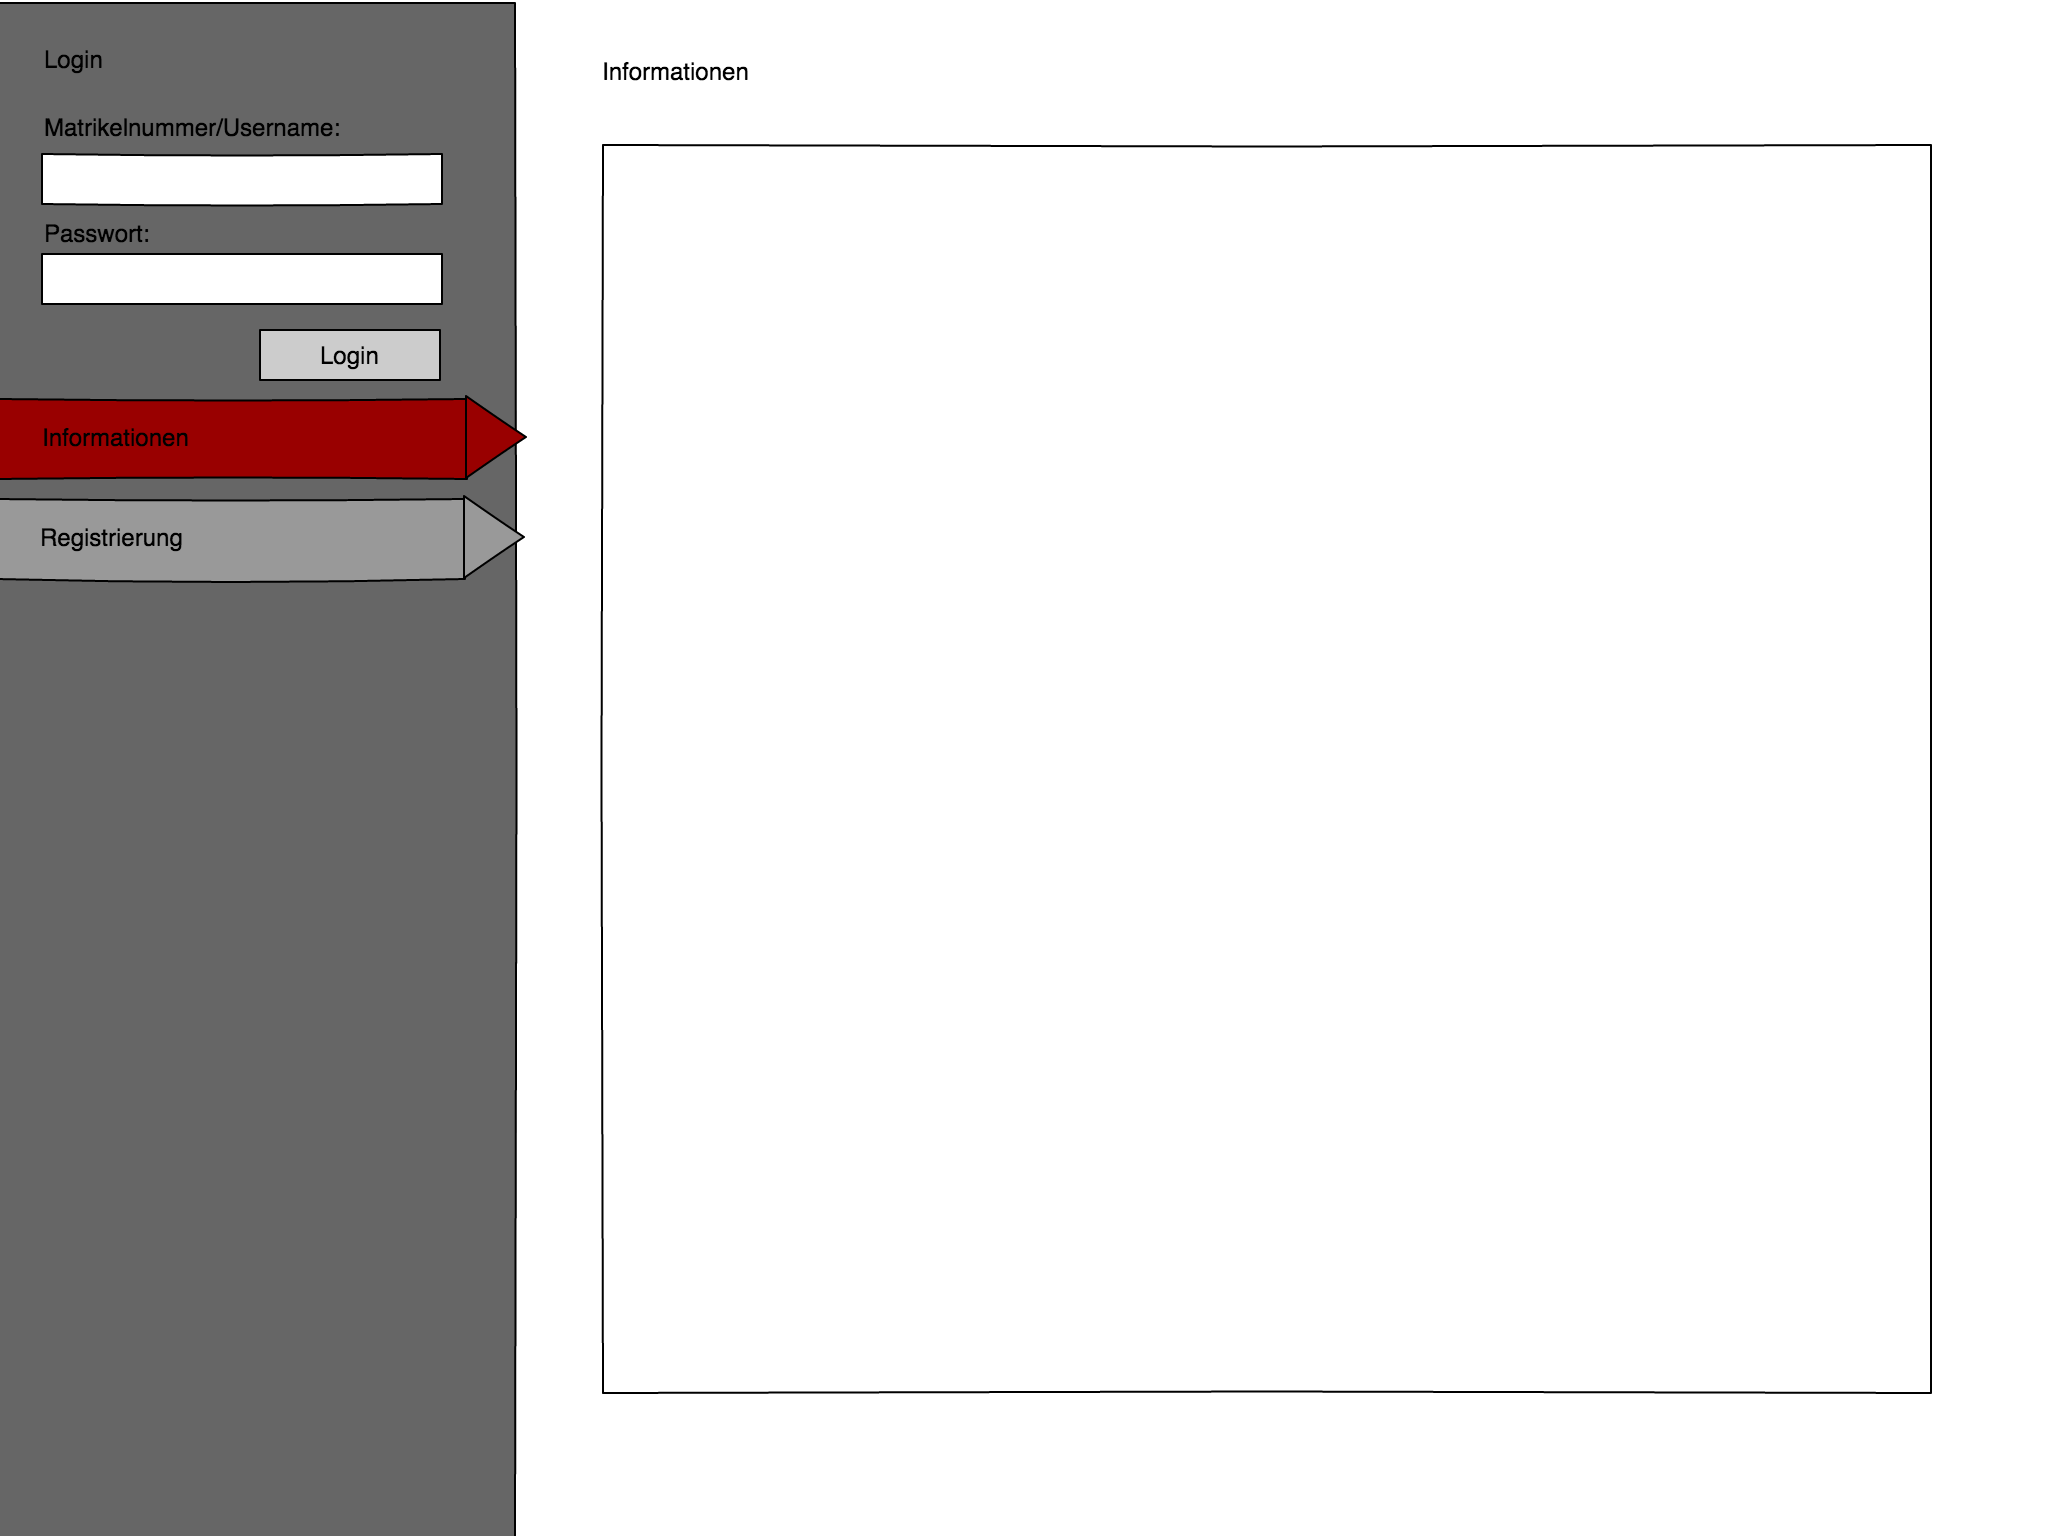
\includegraphics[width=\textwidth,
keepaspectratio=true]{gui/index.png}}
\captionof{figure}{Startseite} \label{GUIindex}
\pagebreak
\fbox{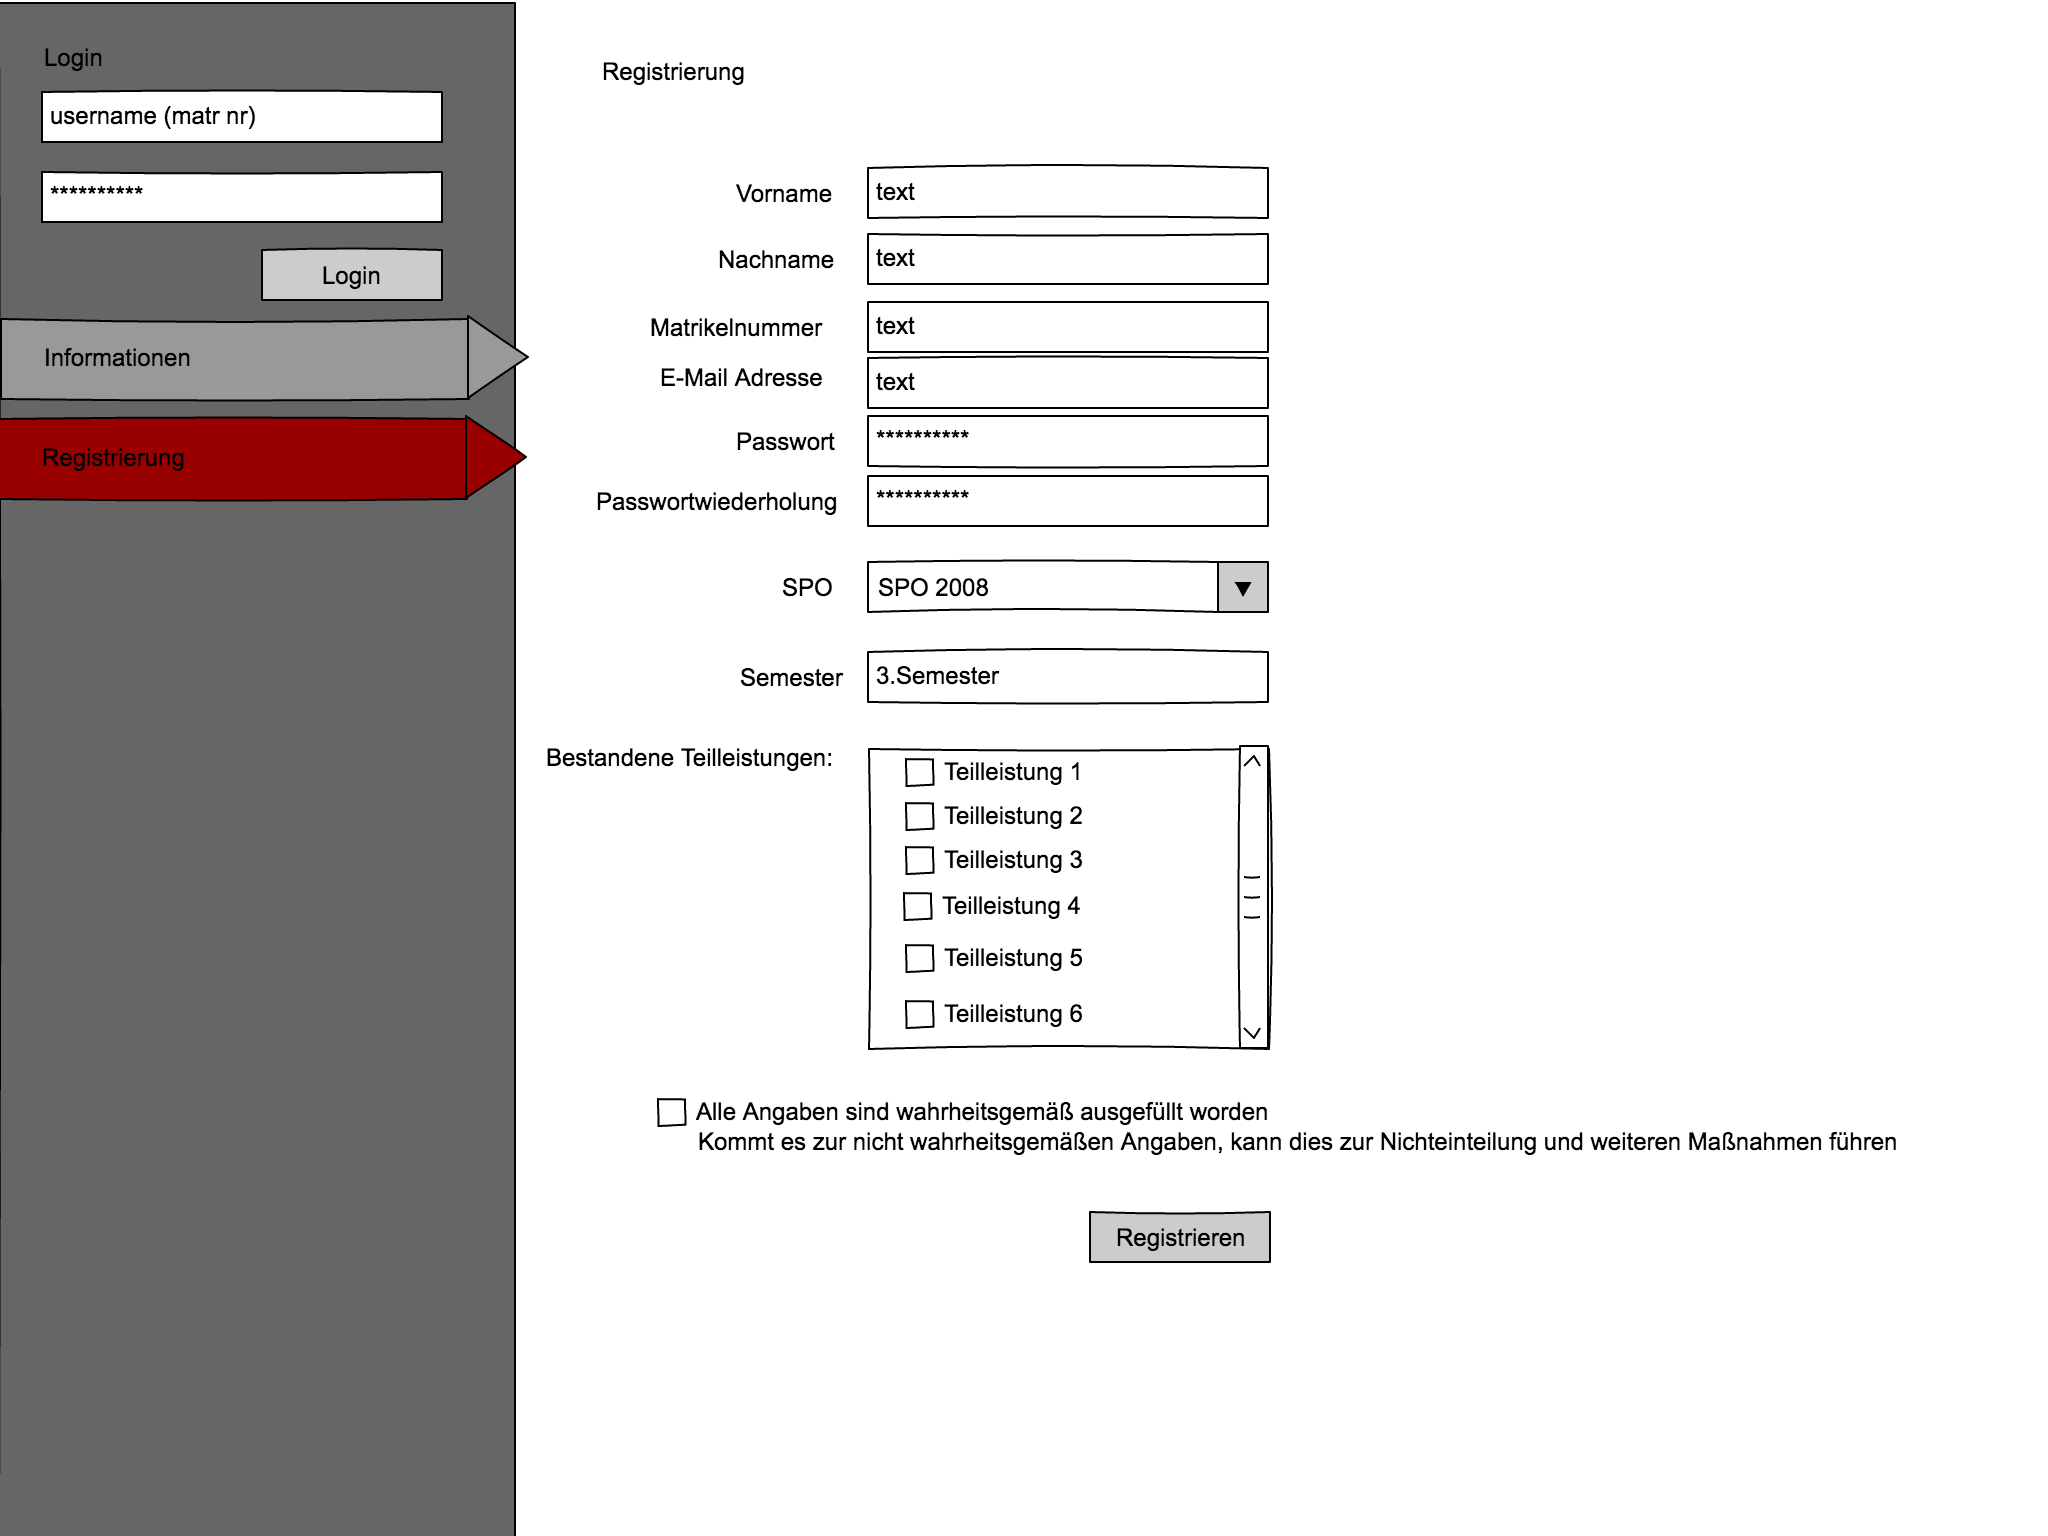
\includegraphics[width=\textwidth,
keepaspectratio=true]{gui/registrierung.png}}
\captionof{figure}{Registrierungsansicht} \label{GUIregi}

\fbox{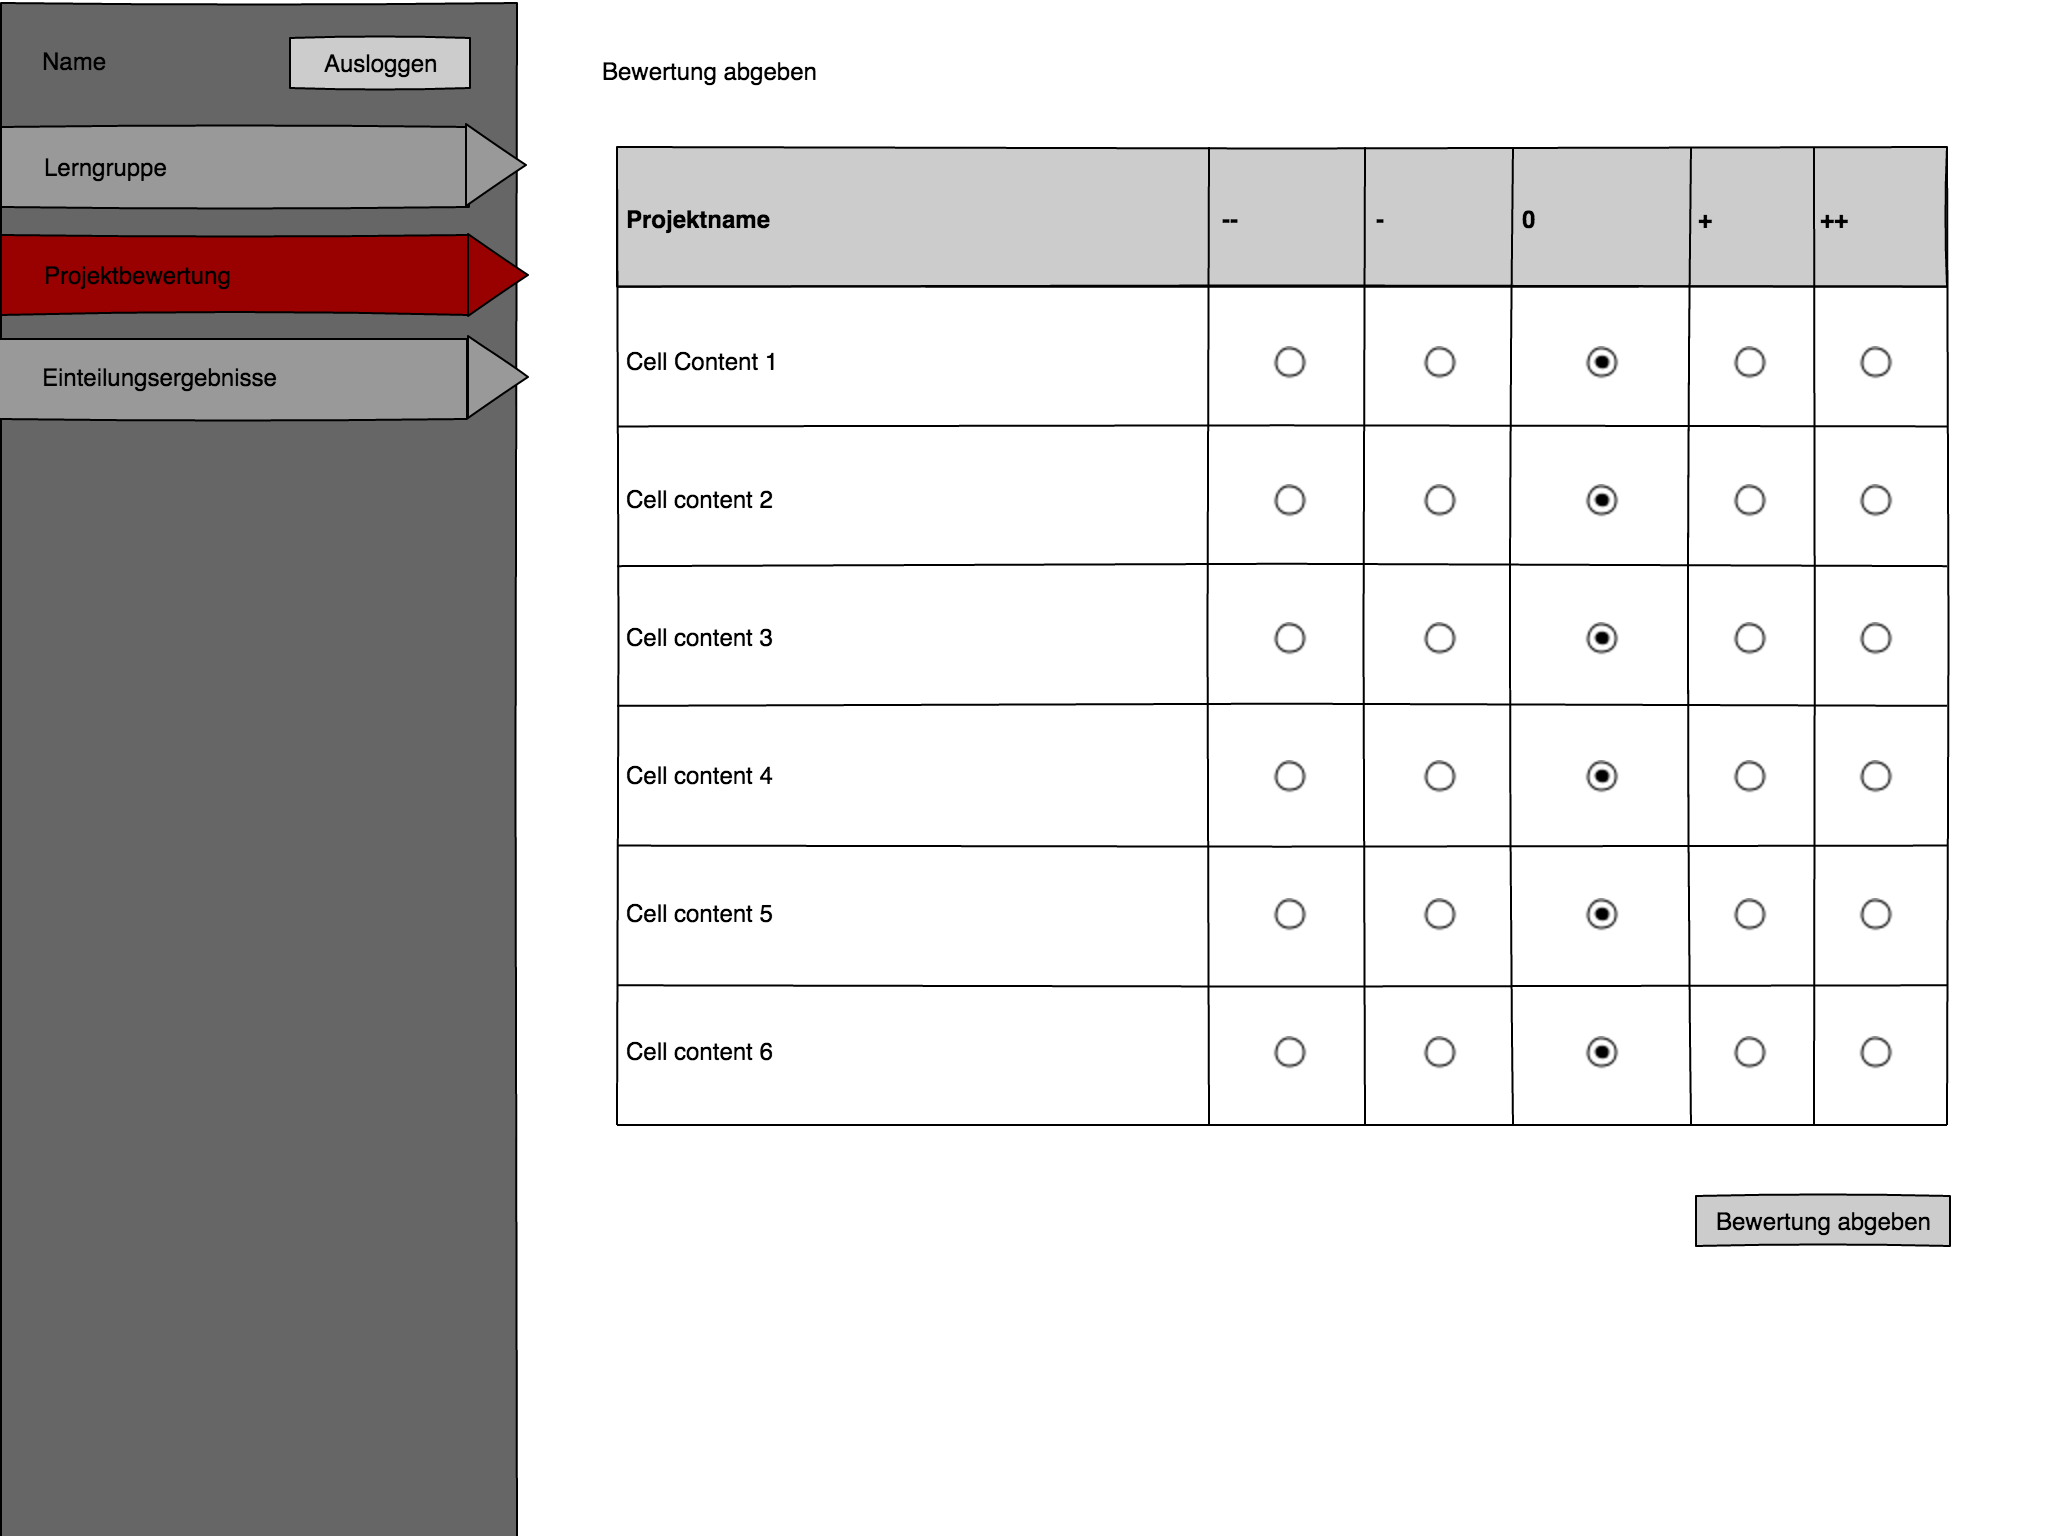
\includegraphics[width=\textwidth,
keepaspectratio=true]{gui/studentbewertung.png}}
\captionof{figure}{\gls{Bewertung}smaske} \label{GUIbewertung}

\fbox{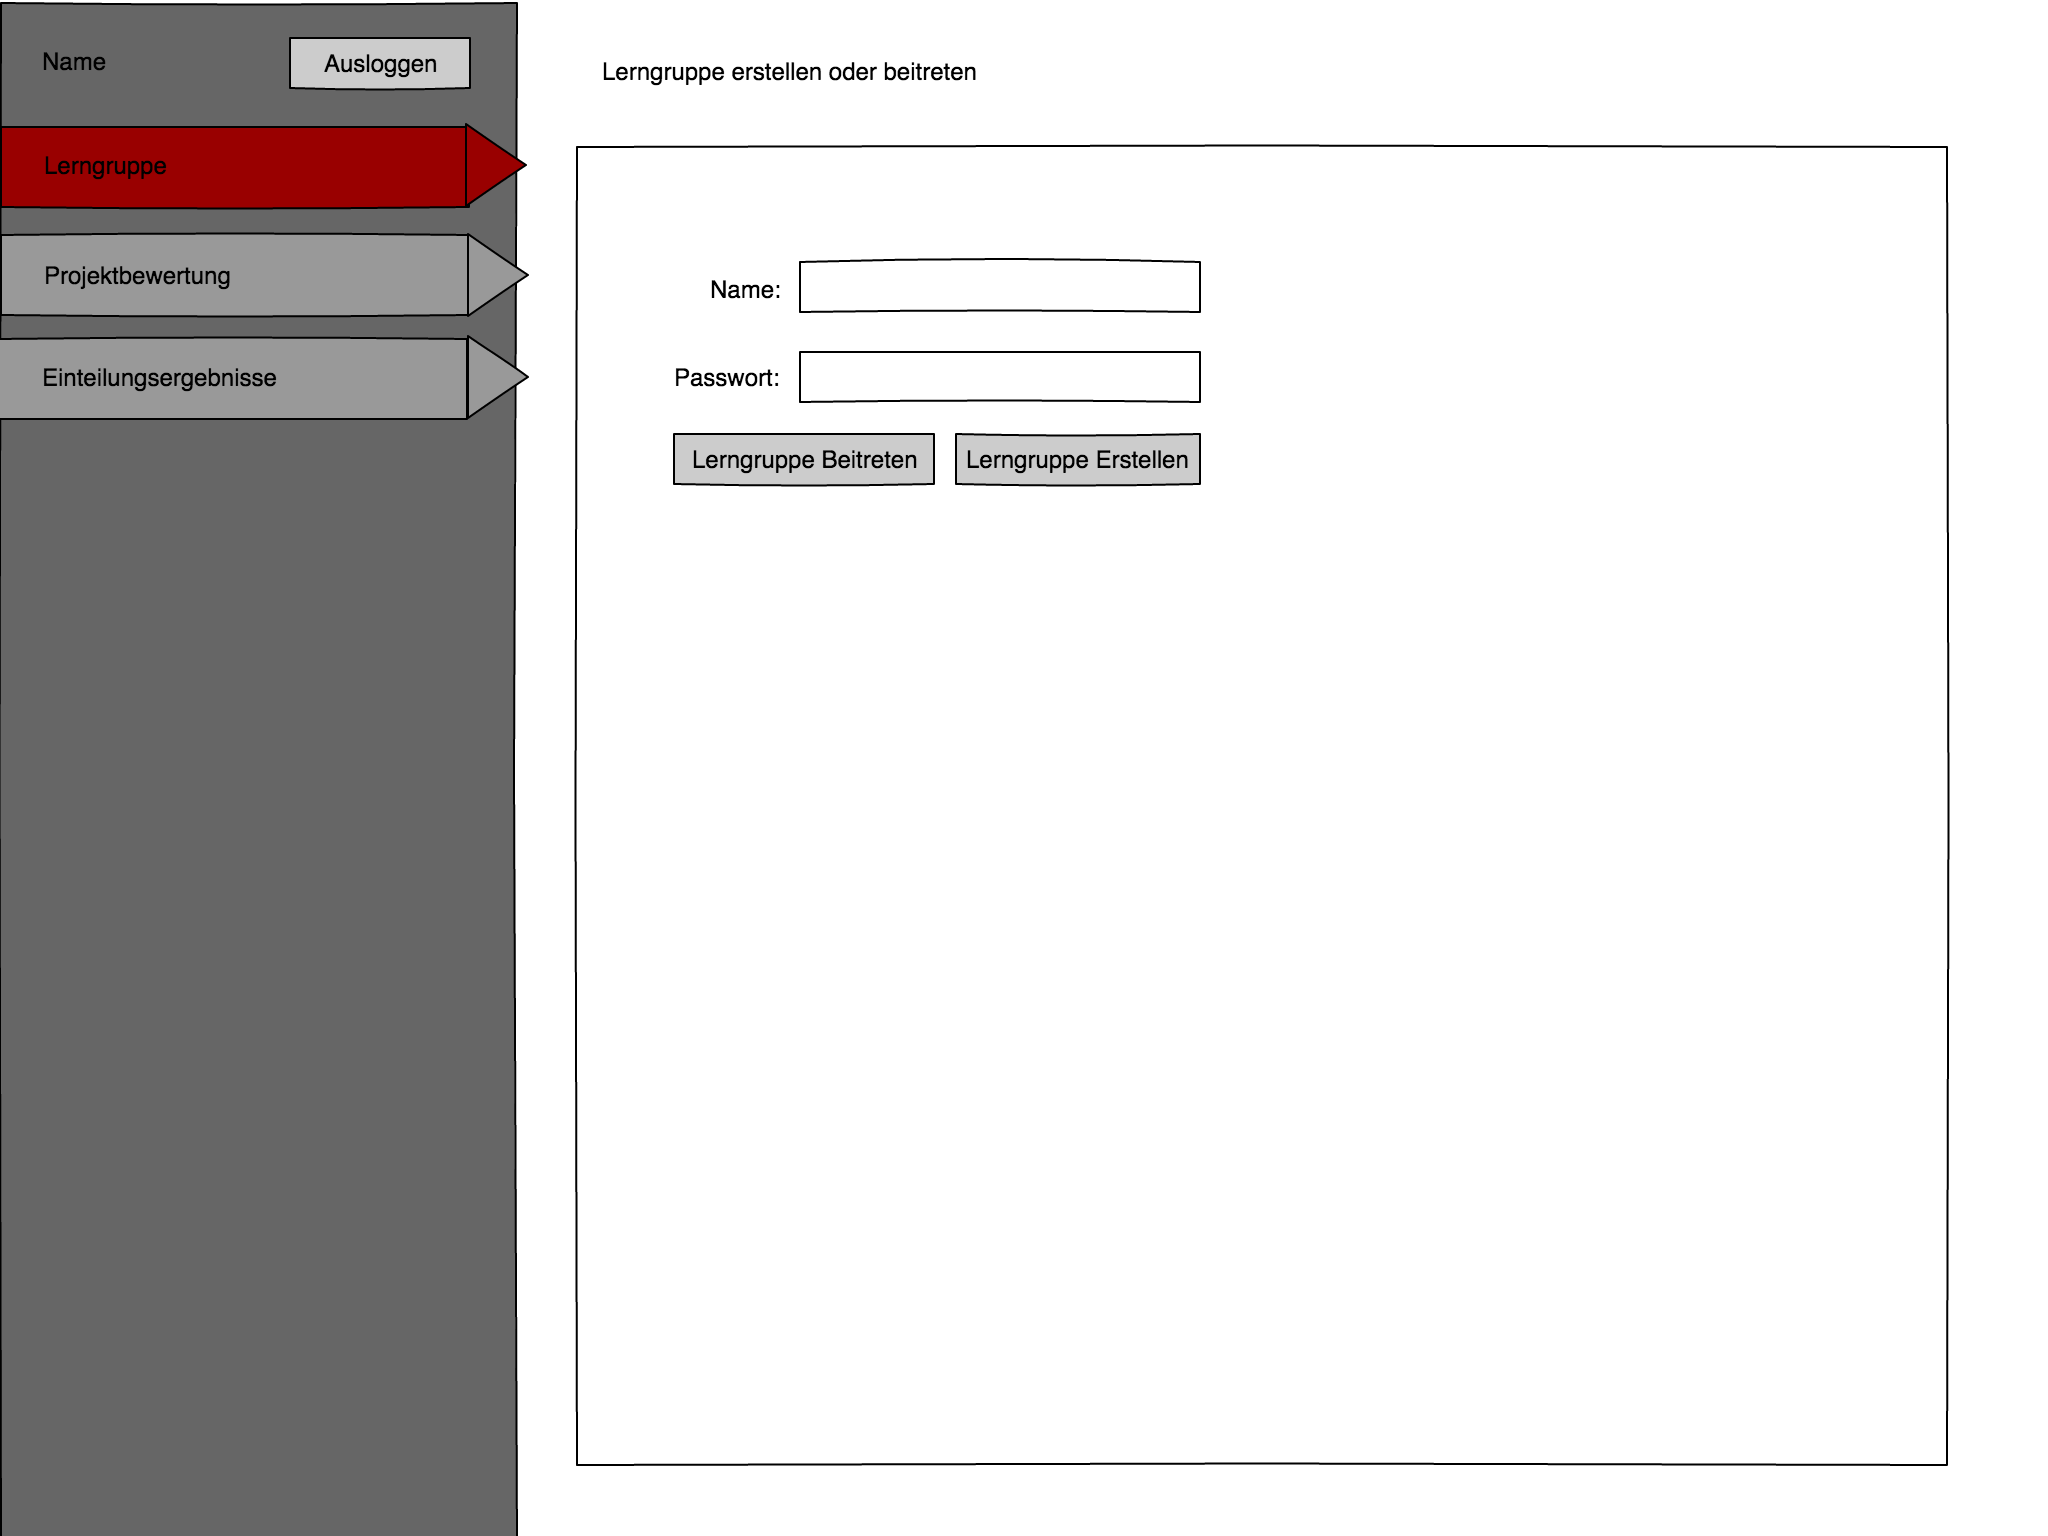
\includegraphics[width=\textwidth,
keepaspectratio=true]{gui/studentlerngruppe.png}}
\captionof{figure}{Anmeldung zu \gls{Lerngruppe}} \label{GUIanmeldLG}
\medskip
\fbox{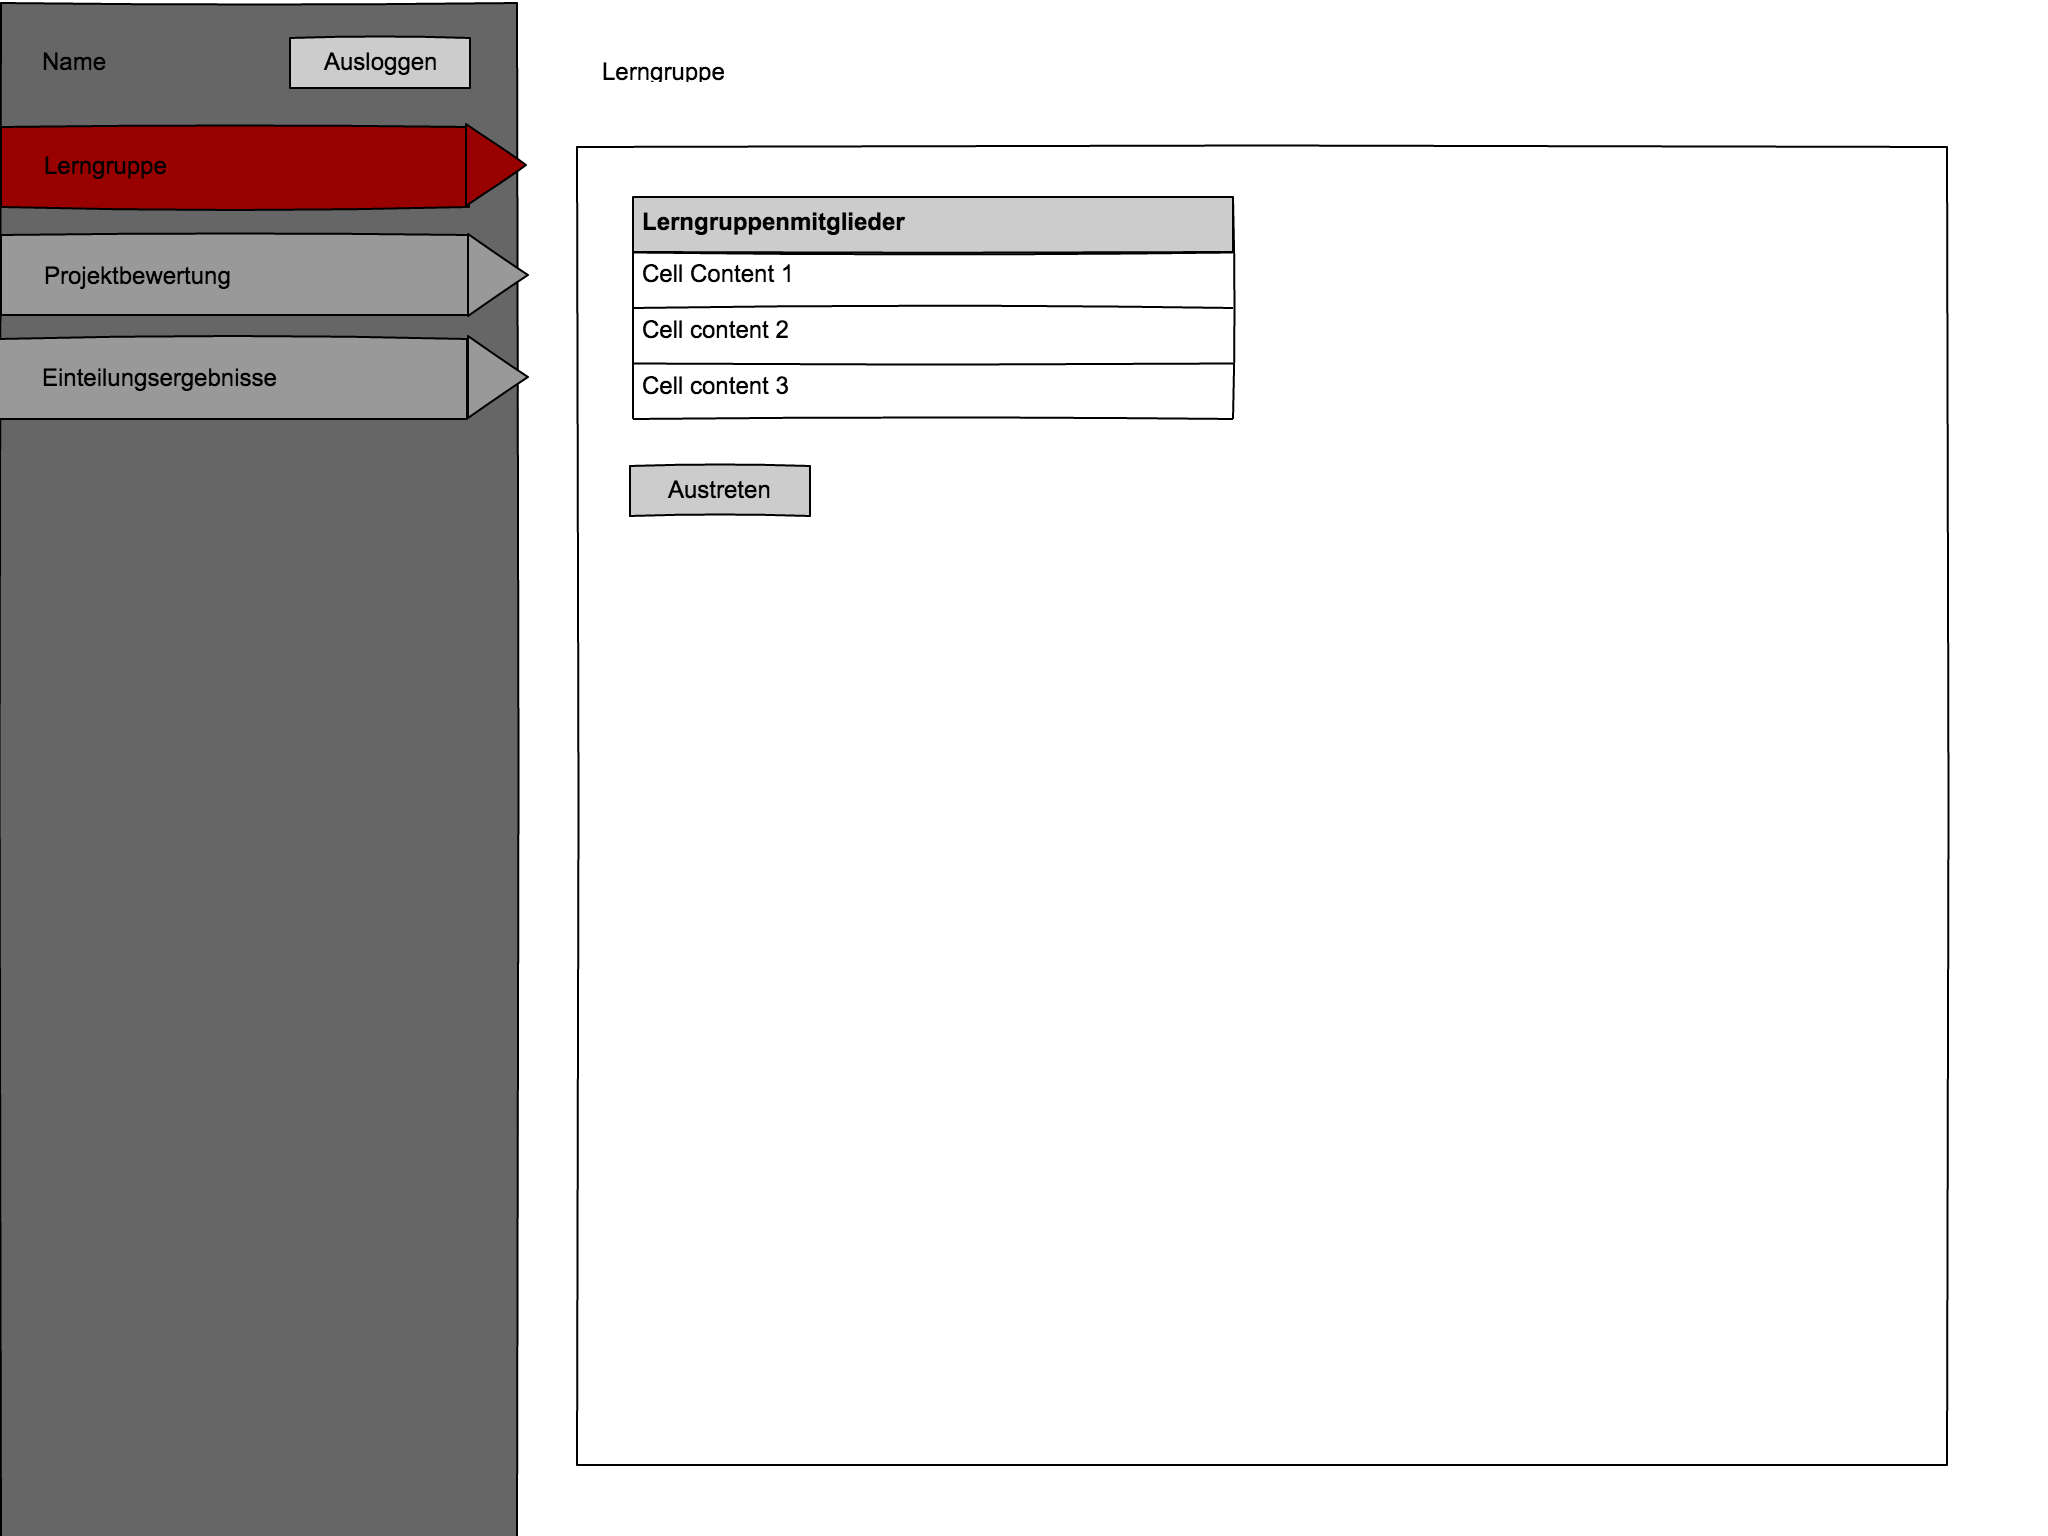
\includegraphics[width=\textwidth,
keepaspectratio=true]{gui/studentlerngruppeingr.png}}
\captionof{figure}{\glspl{Lerngruppe}übersicht} \label{GUIlerngUebersicht}
\medskip
\fbox{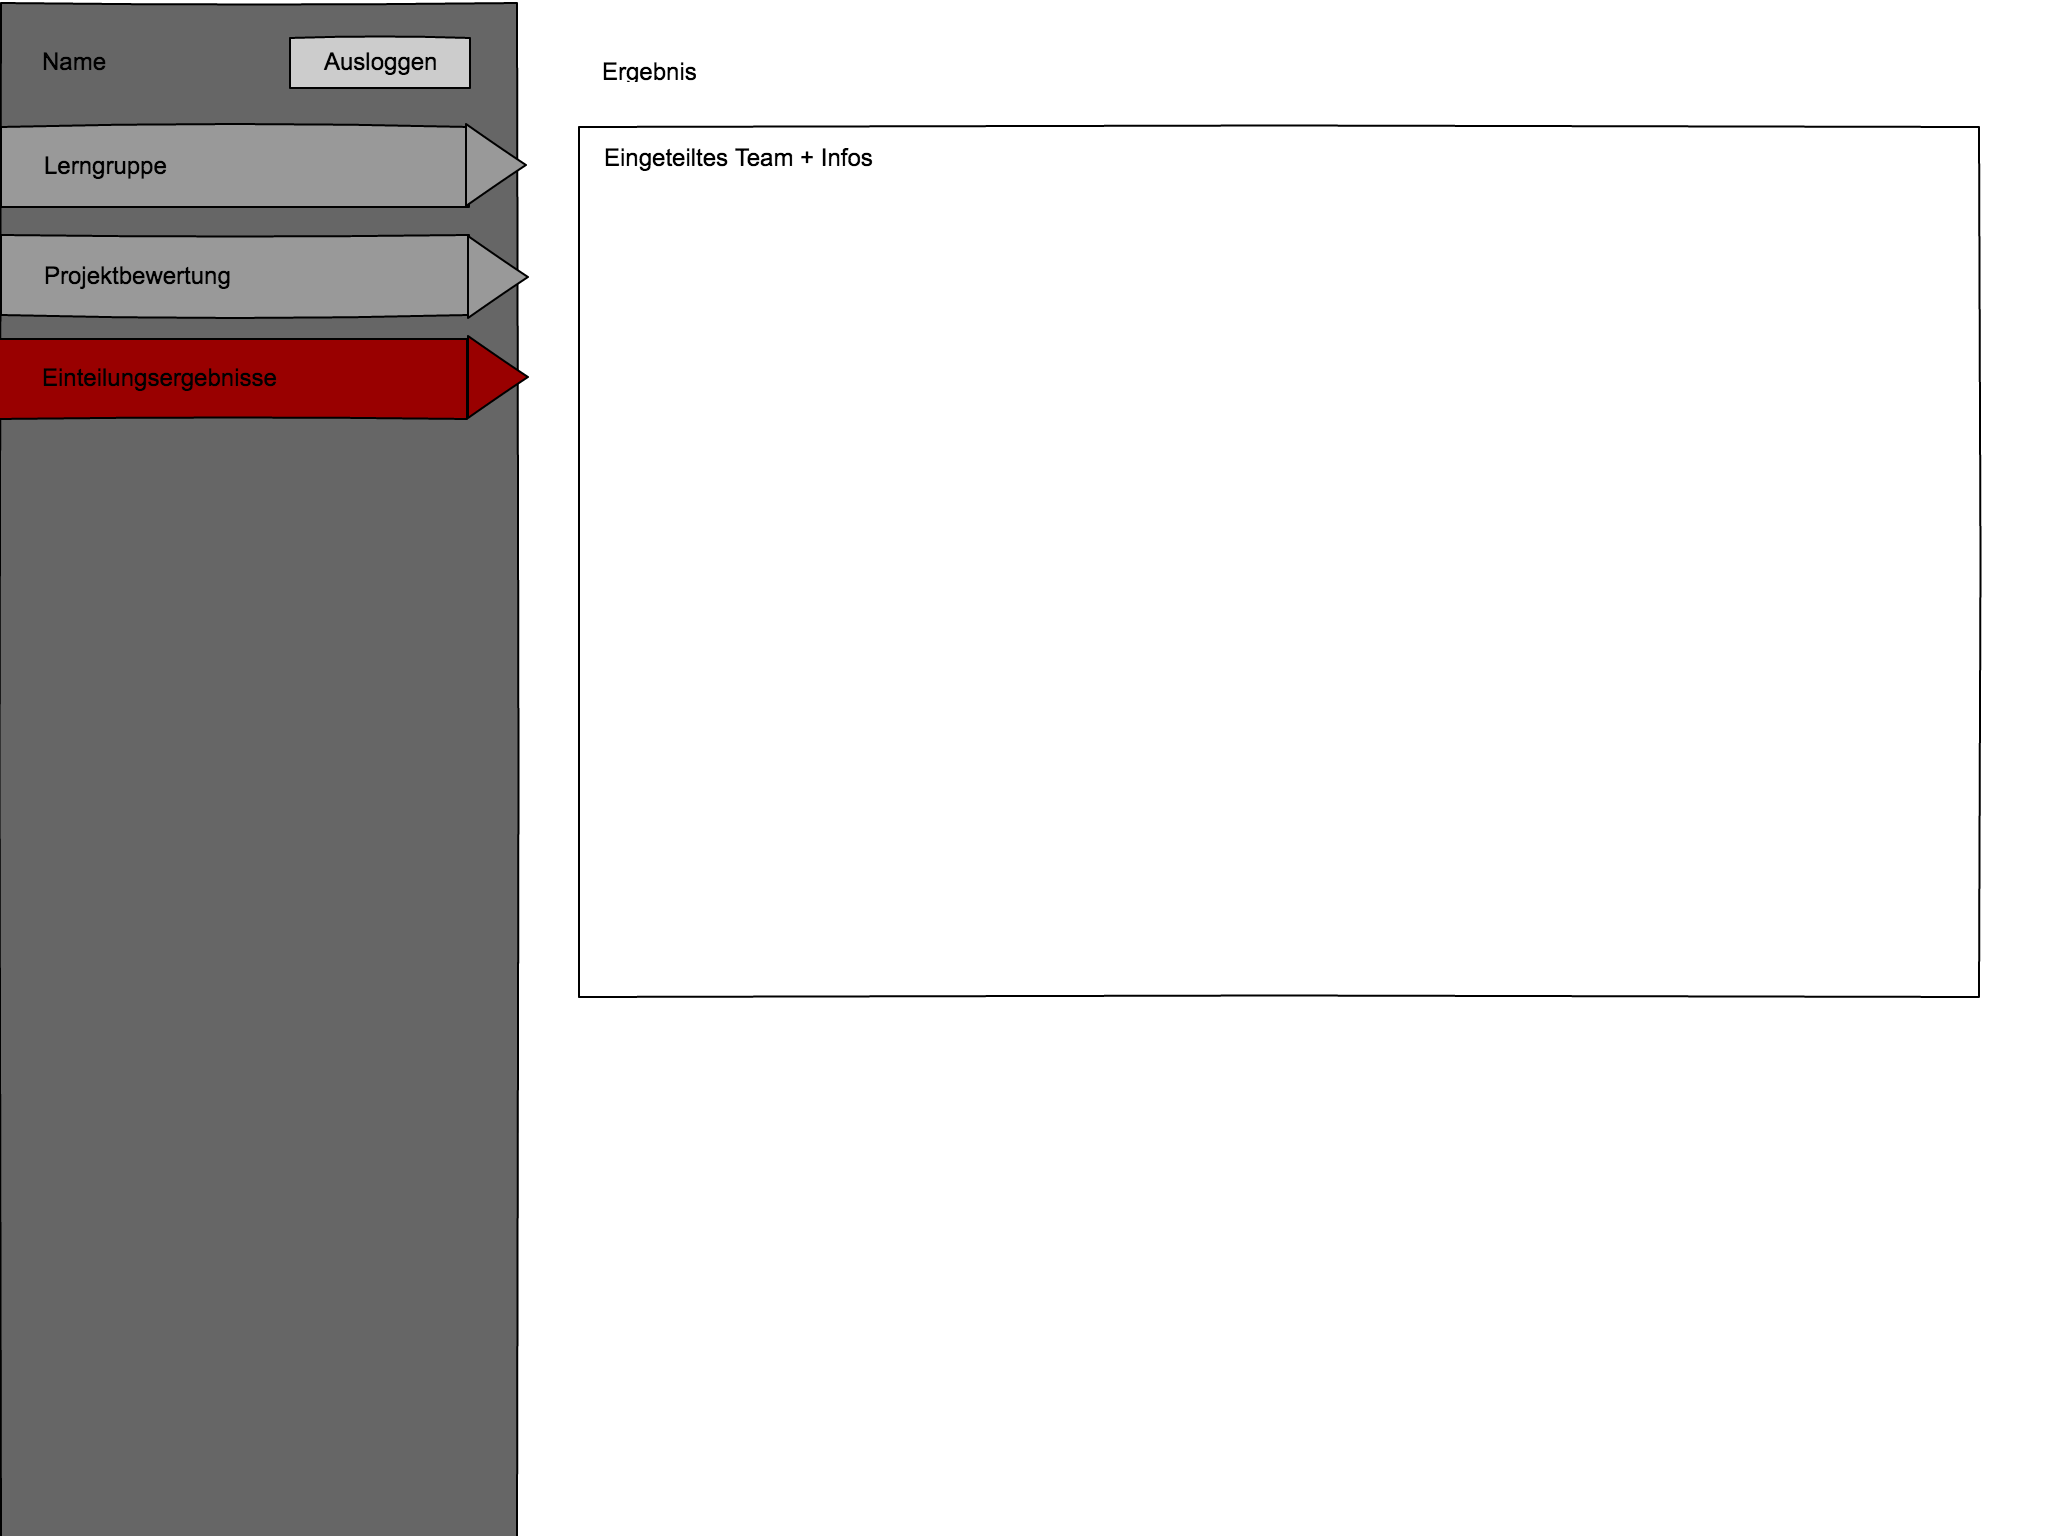
\includegraphics[width=\textwidth,
keepaspectratio=true]{gui/studentergebnis.png}}
\captionof{figure}{Ergebnisansicht} \label{GUIergebnisAnsicht}
\medskip
\fbox{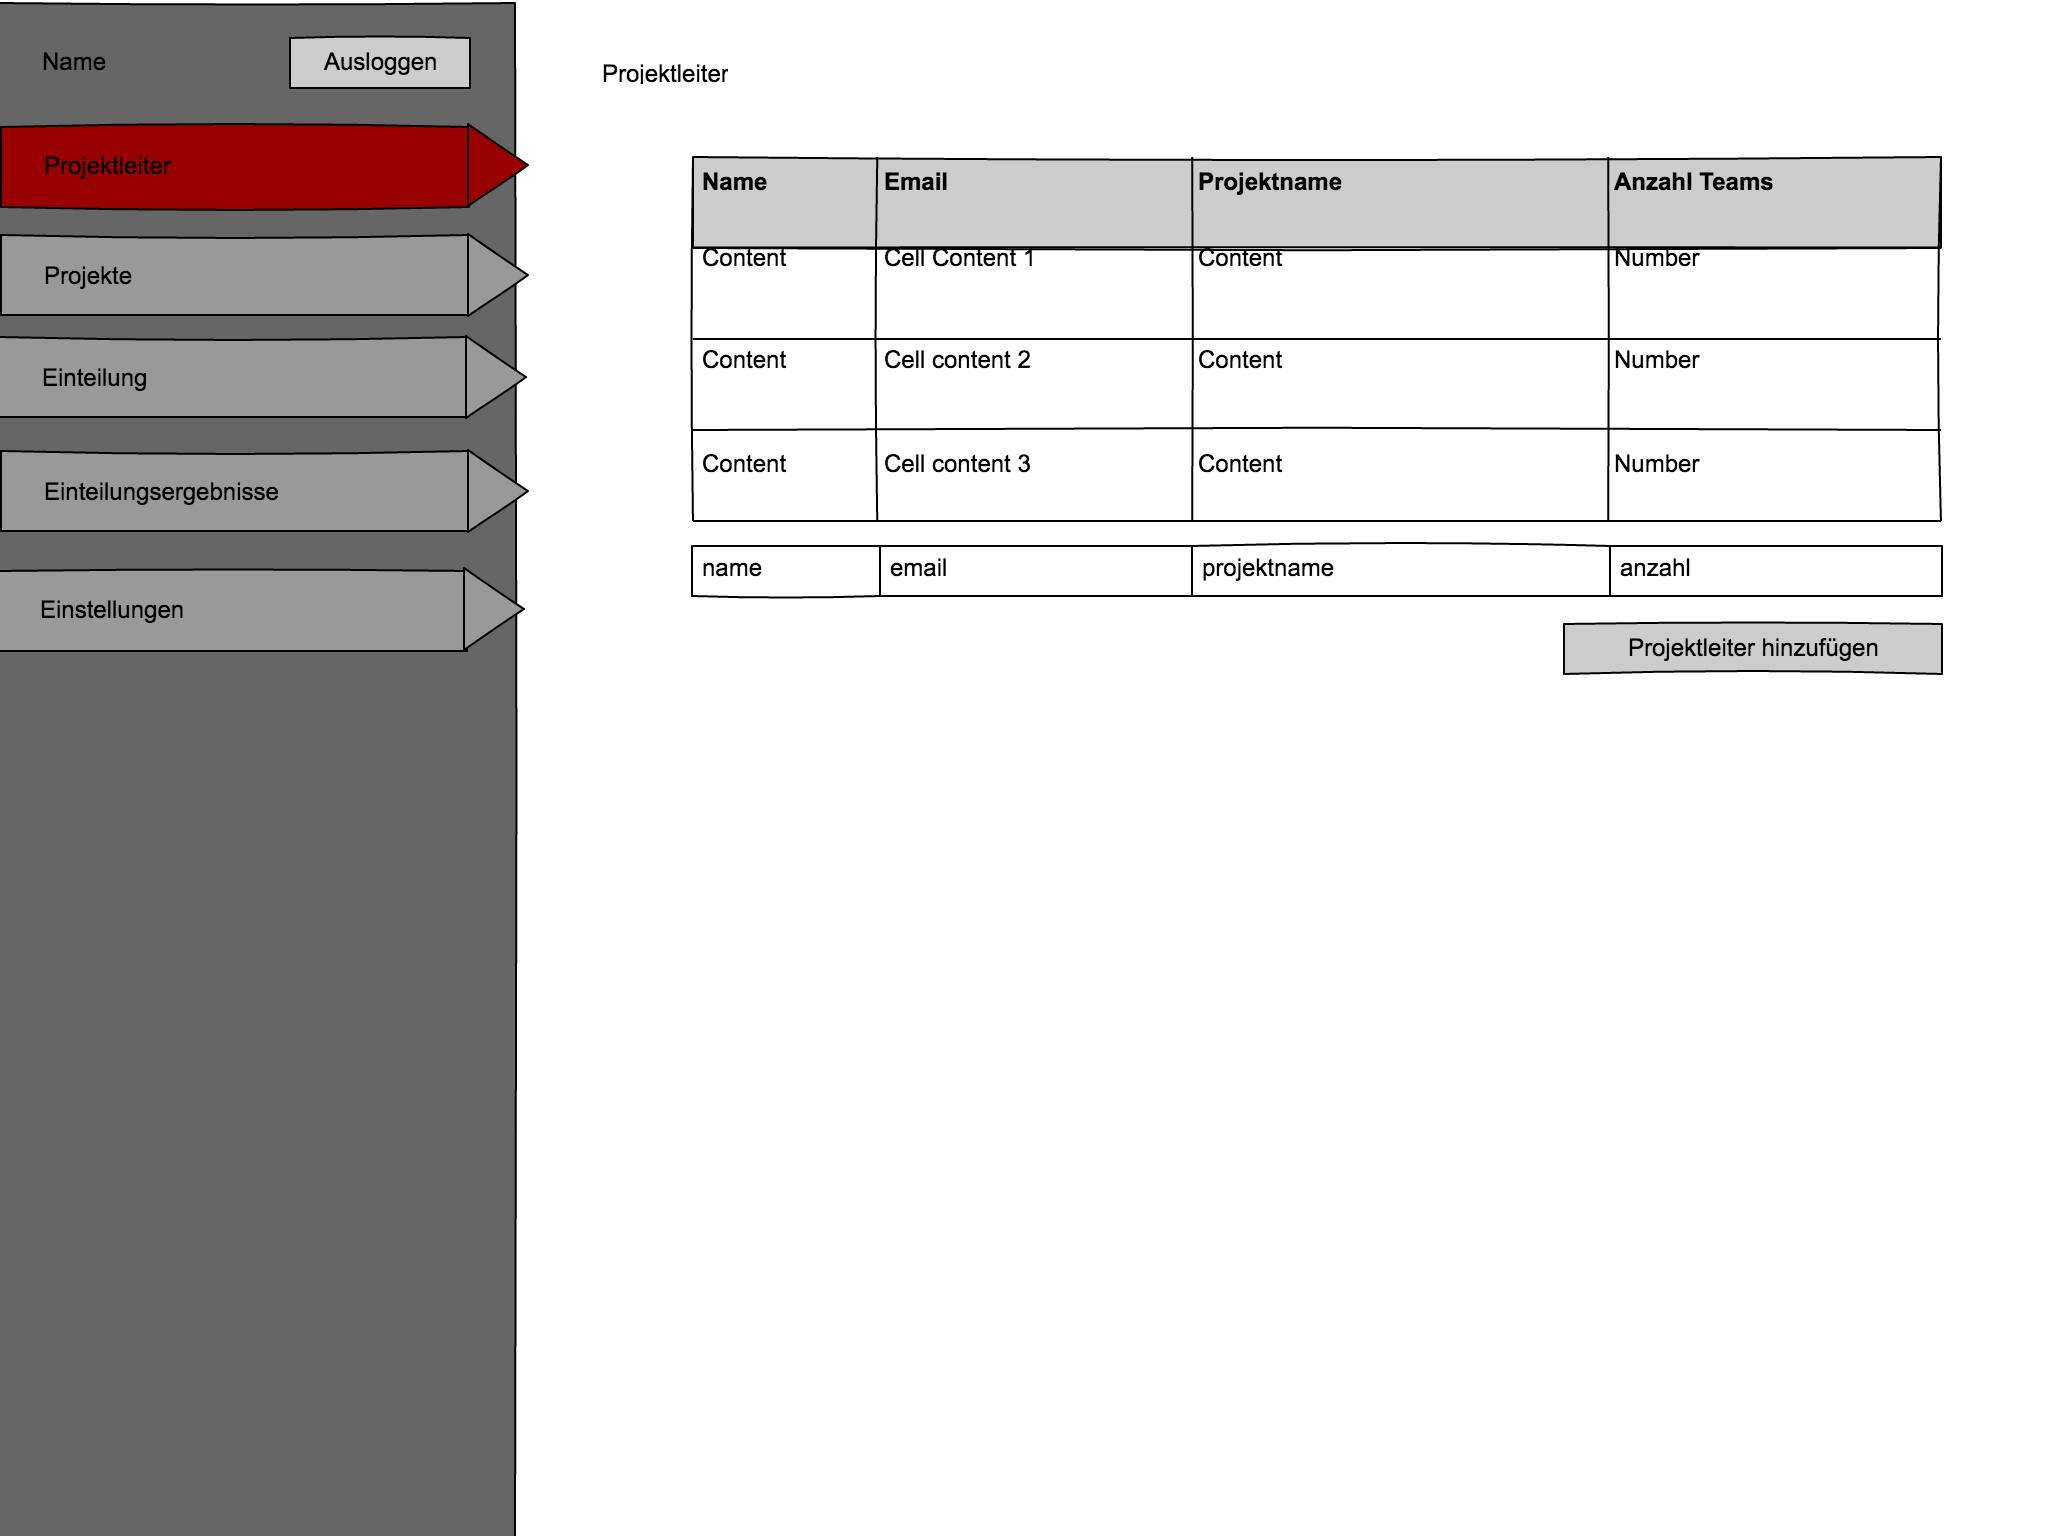
\includegraphics[width=\textwidth,
keepaspectratio=true]{gui/adminprojleiter.png}}
\captionof{figure}{\gls{Projektbetreuer}übersicht} \label{GUIprojLeiterUebersicht}
\medskip
\fbox{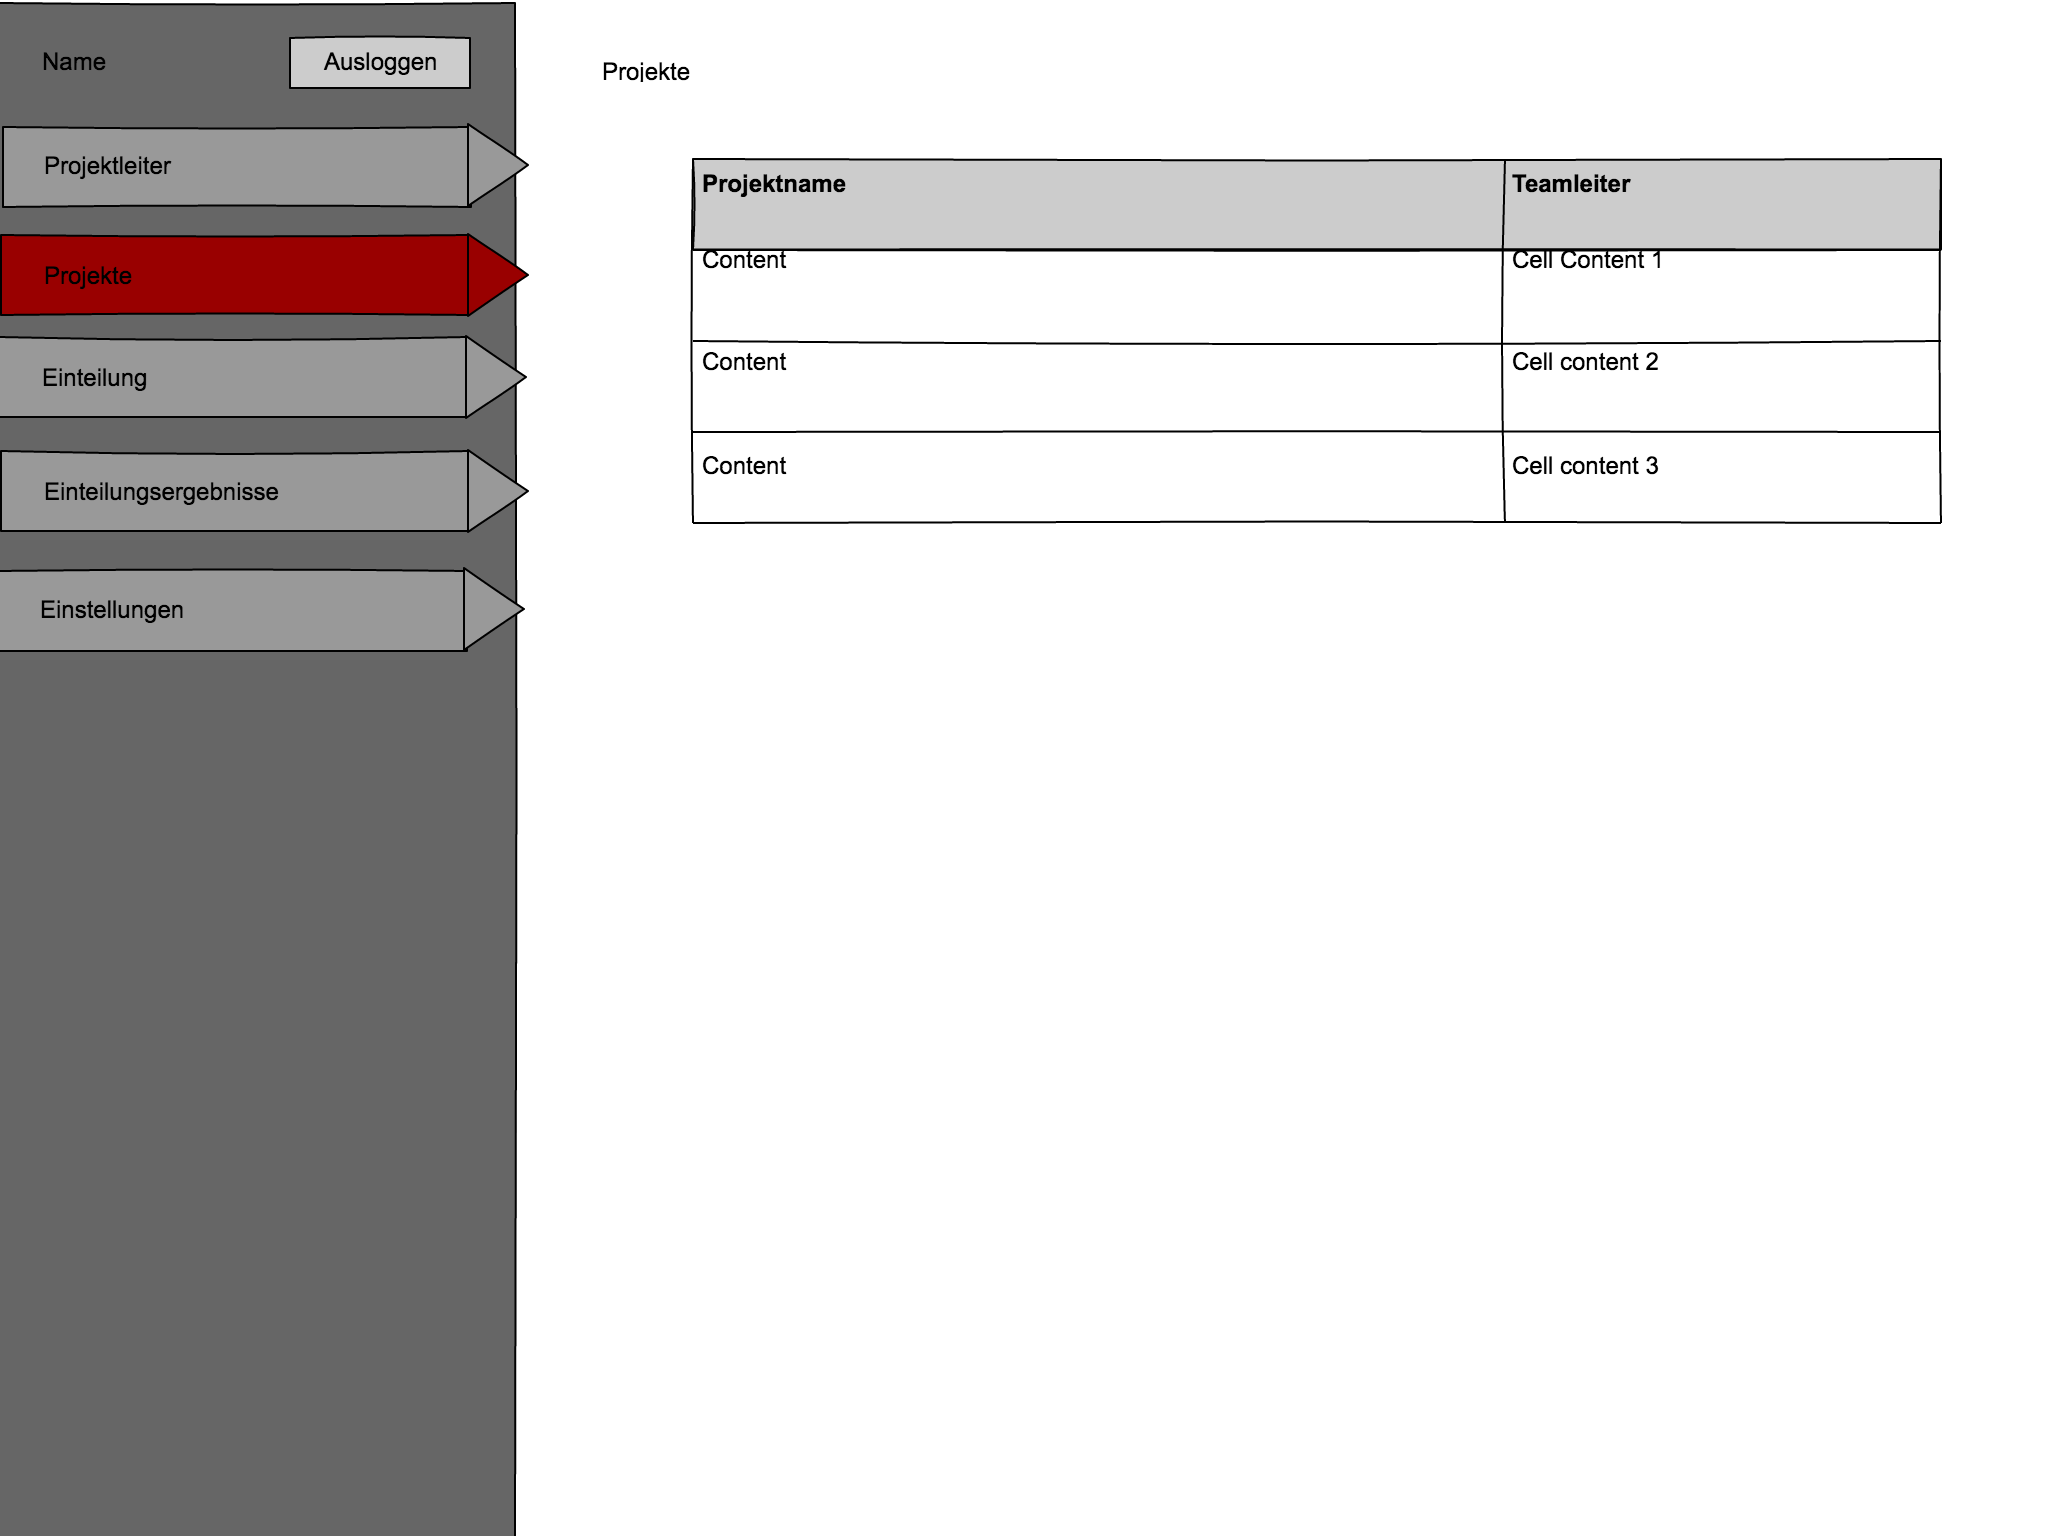
\includegraphics[width=\textwidth,
keepaspectratio=true]{gui/adminprojekte.png}}
\captionof{figure}{\gls{Projekt}übersicht} \label{GUIprojUebersicht}
\fbox{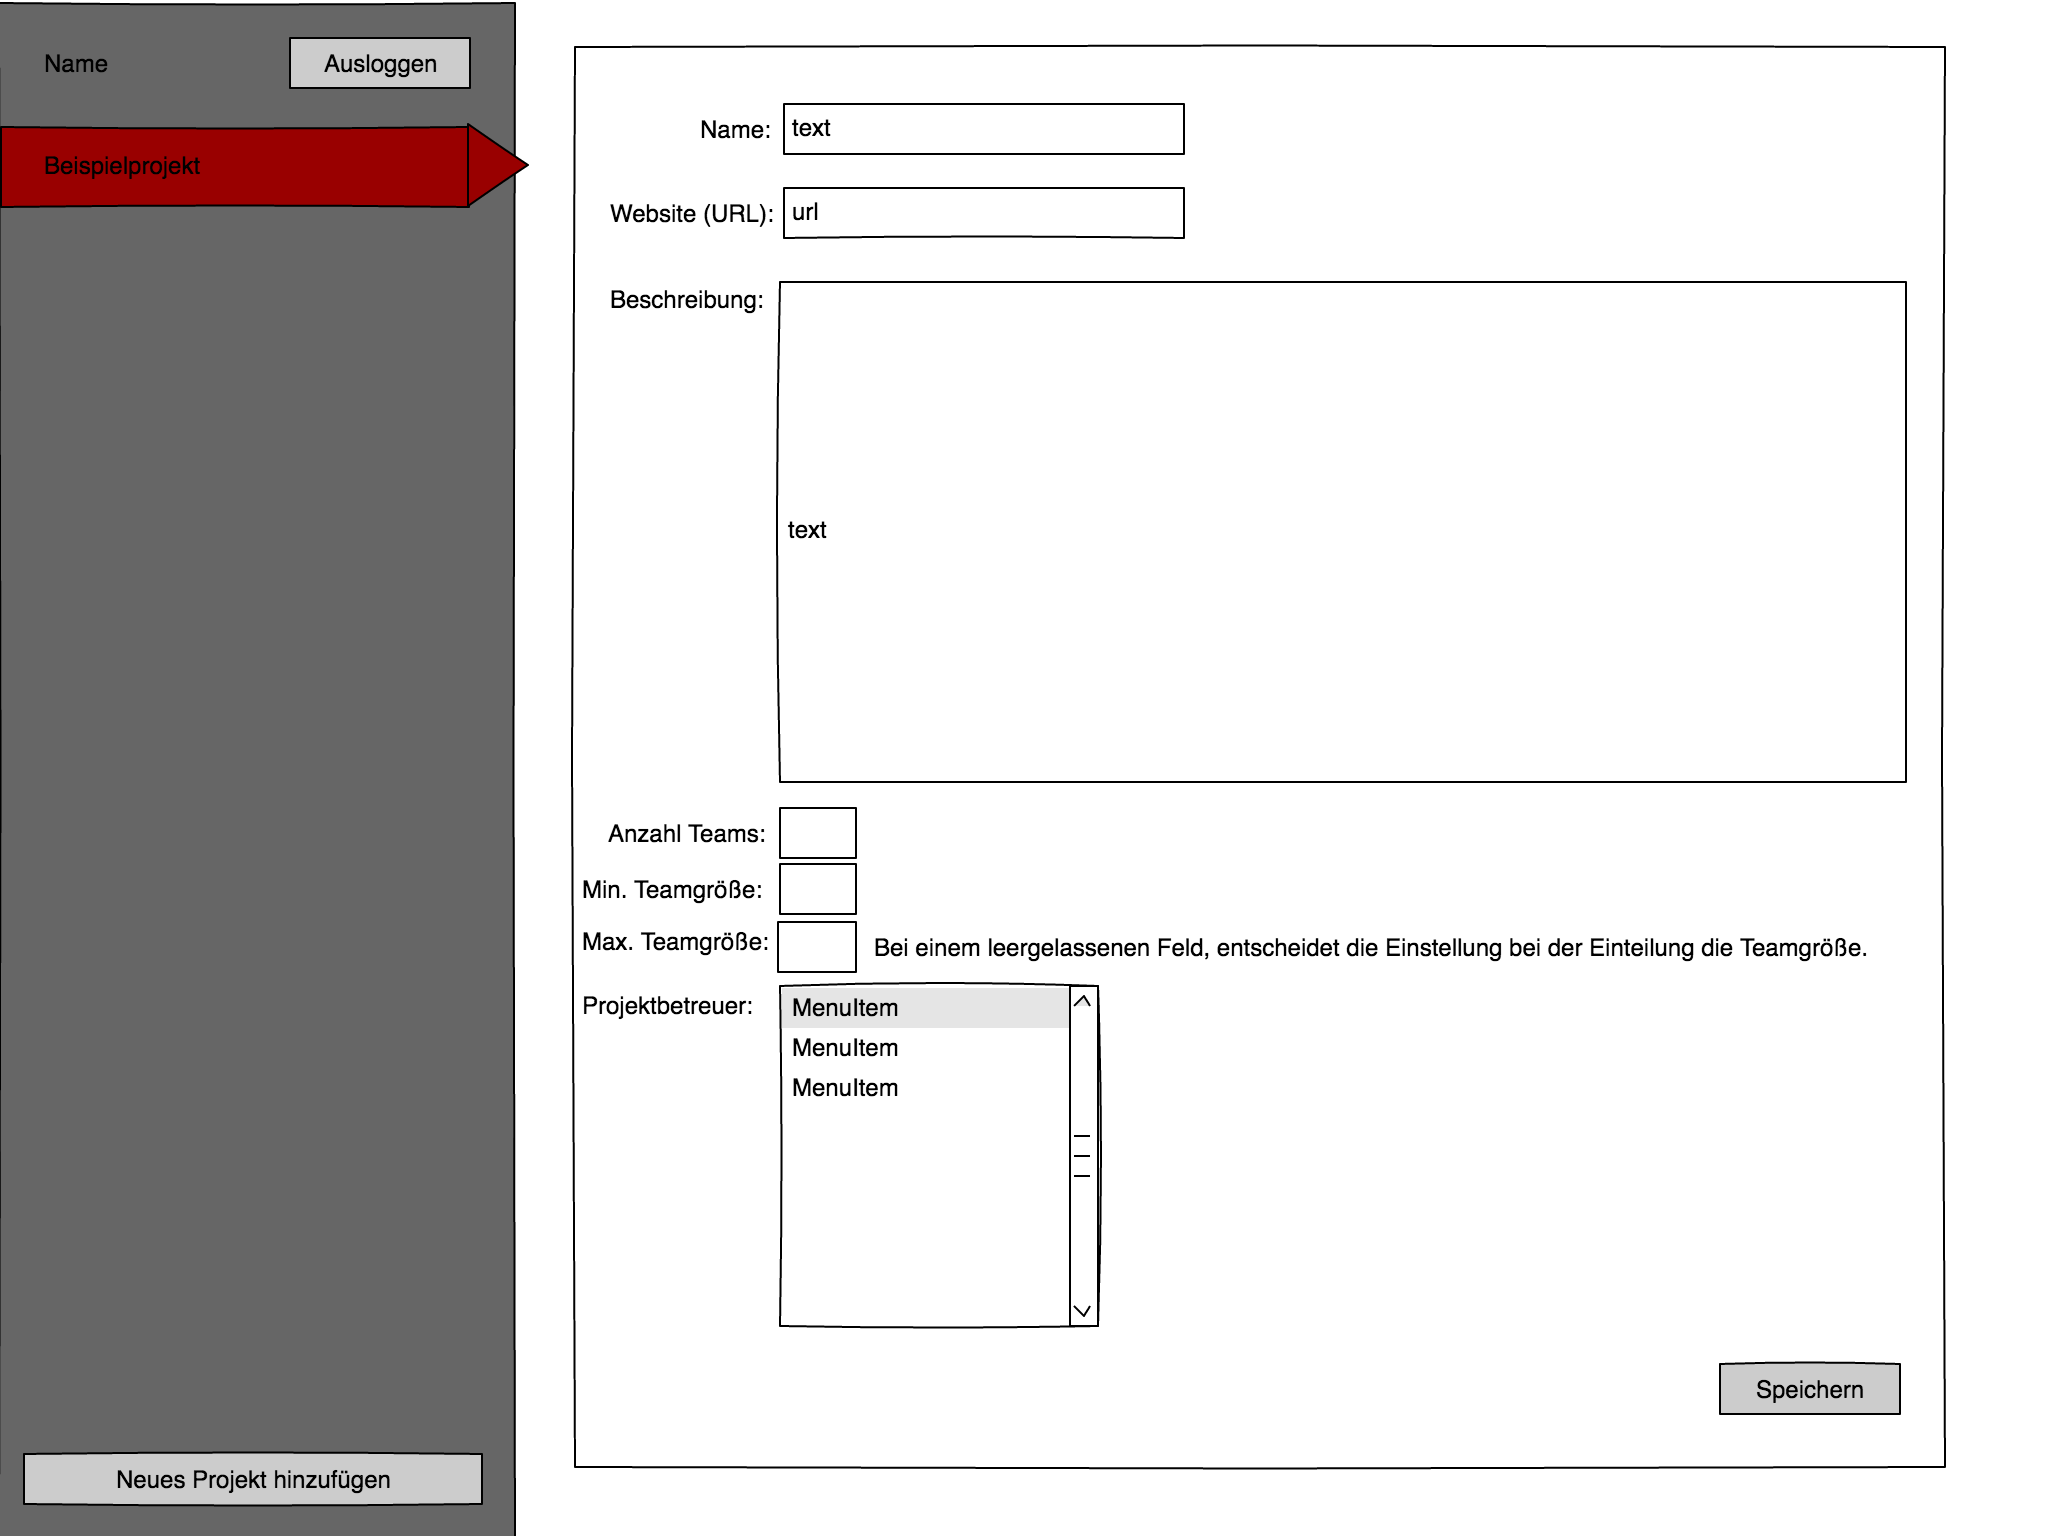
\includegraphics[width=\textwidth,
keepaspectratio=true]{gui/projleiterprojekteedit.png}}
\captionof{figure}{\gls{Projekt}eingabe} \label{GUIprojEdit}

\medskip
\fbox{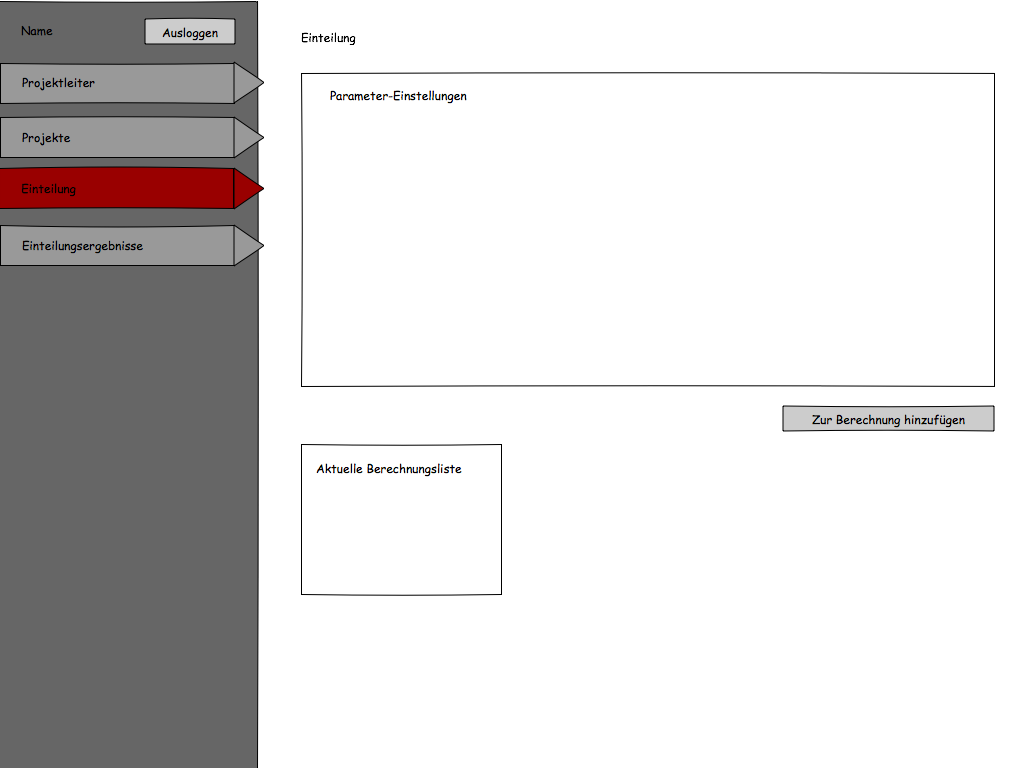
\includegraphics[width=\textwidth,
keepaspectratio=true]{gui/admineinteilung.png}}
\captionof{figure}{Einteilungsmaske} \label{GUIeinteilung}
\medskip
\fbox{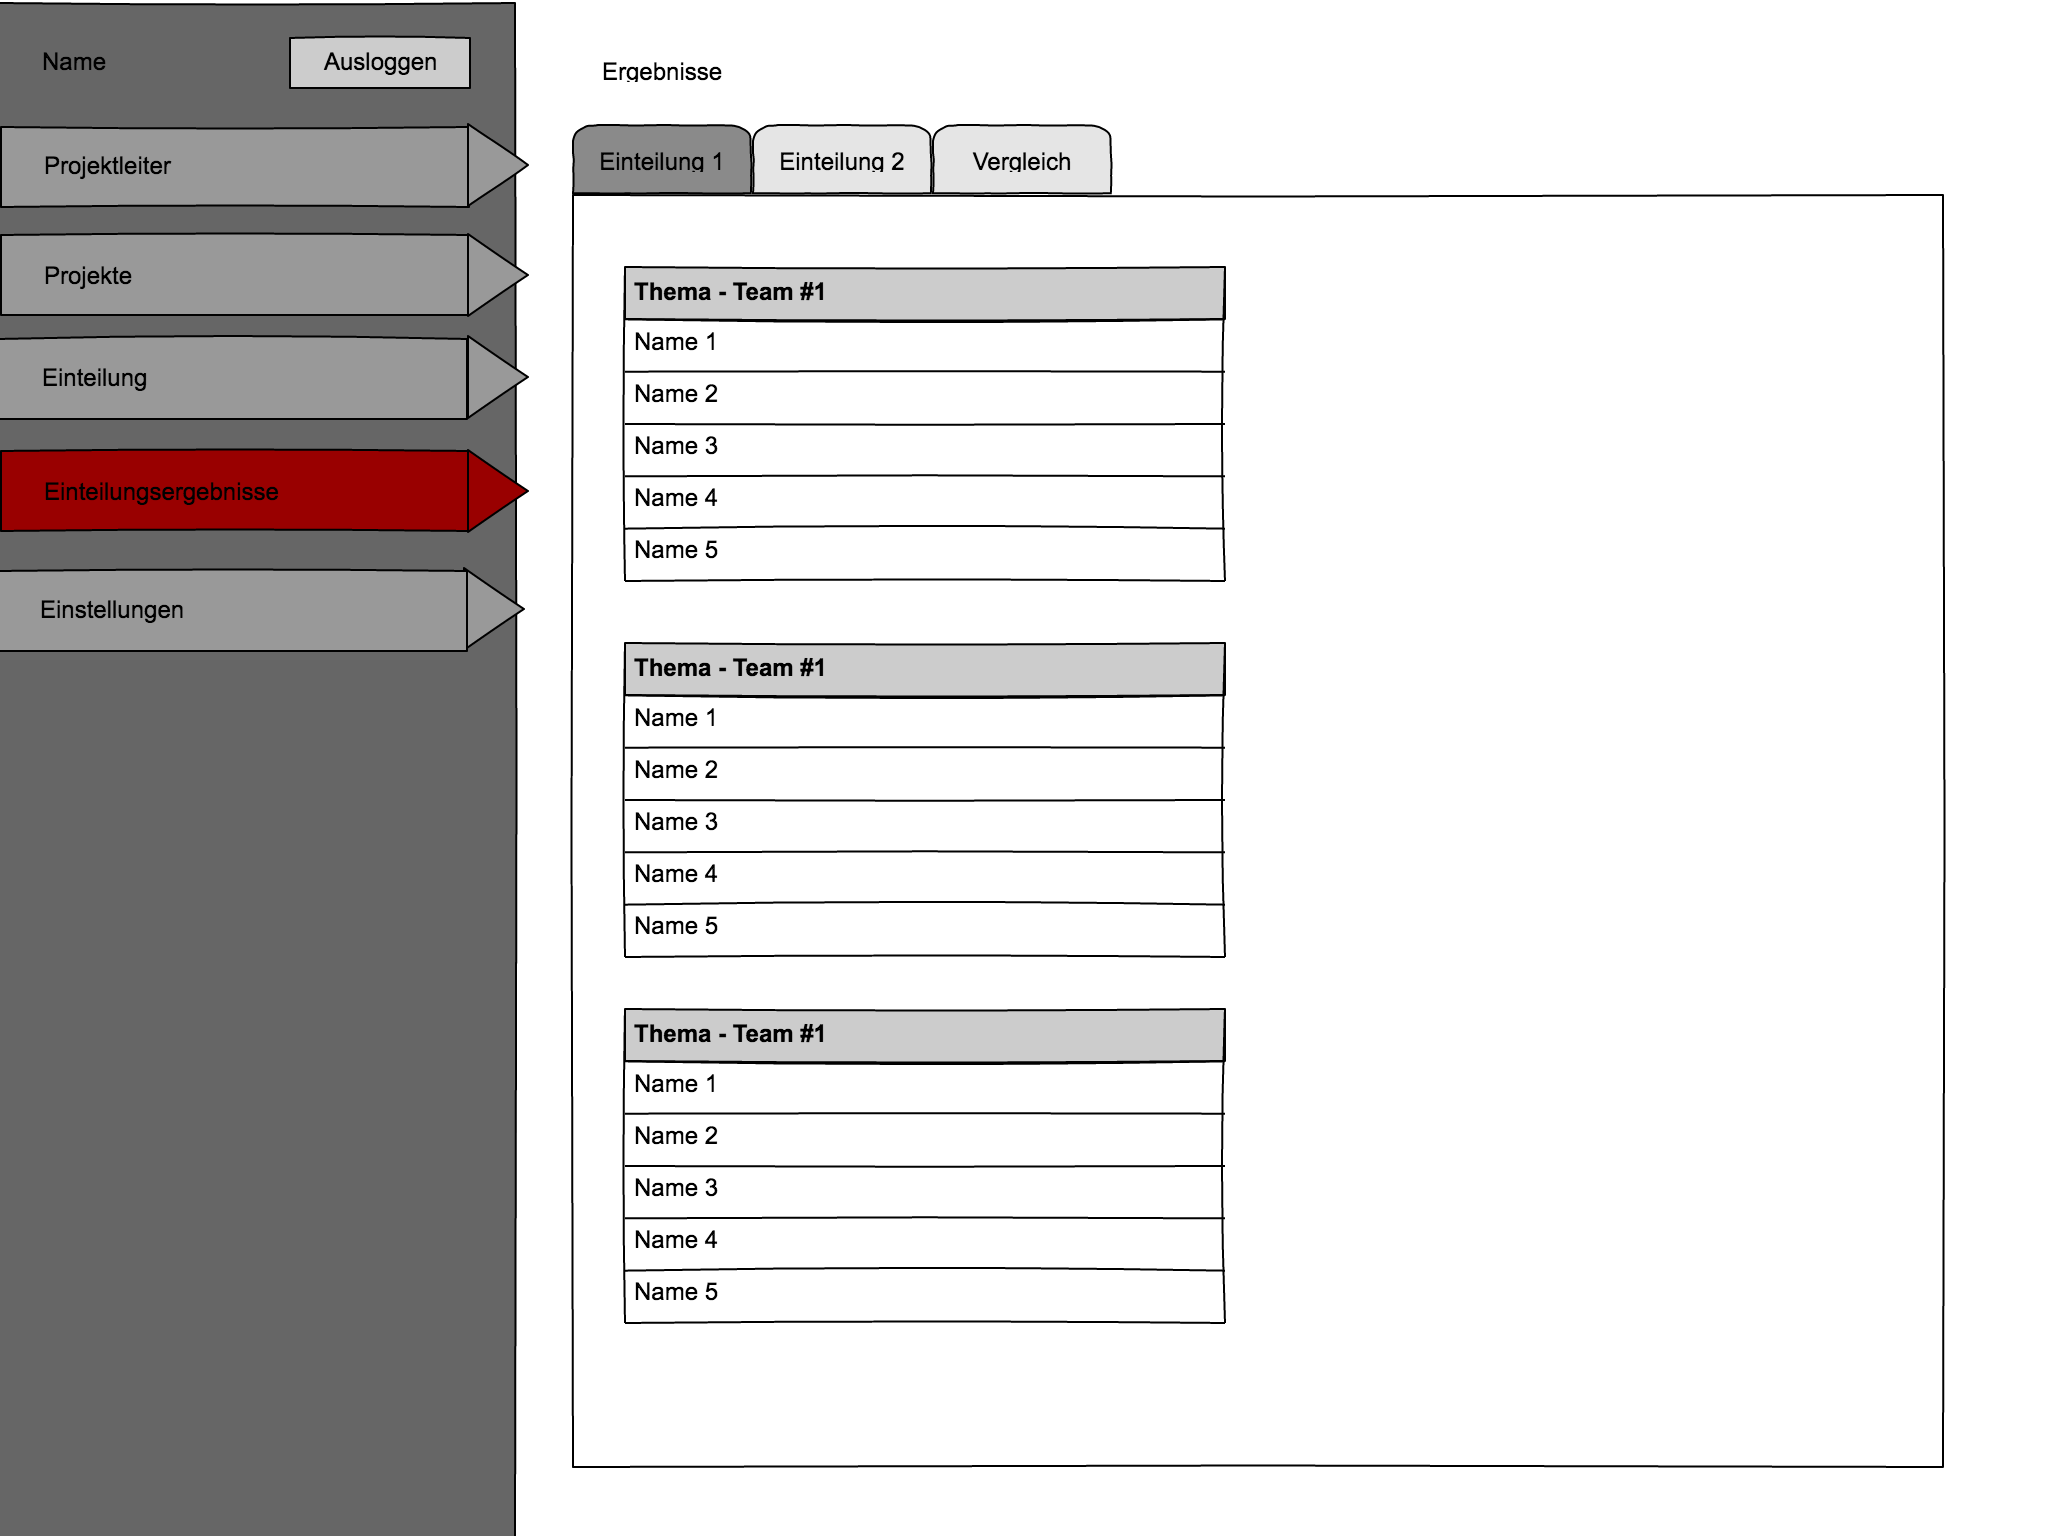
\includegraphics[width=\textwidth,
keepaspectratio=true]{gui/adminergebnisse.png}}
\captionof{figure}{Übersicht der \glspl{Einteilung}} \label{GUIeinteilungErgeb}
\medskip
\fbox{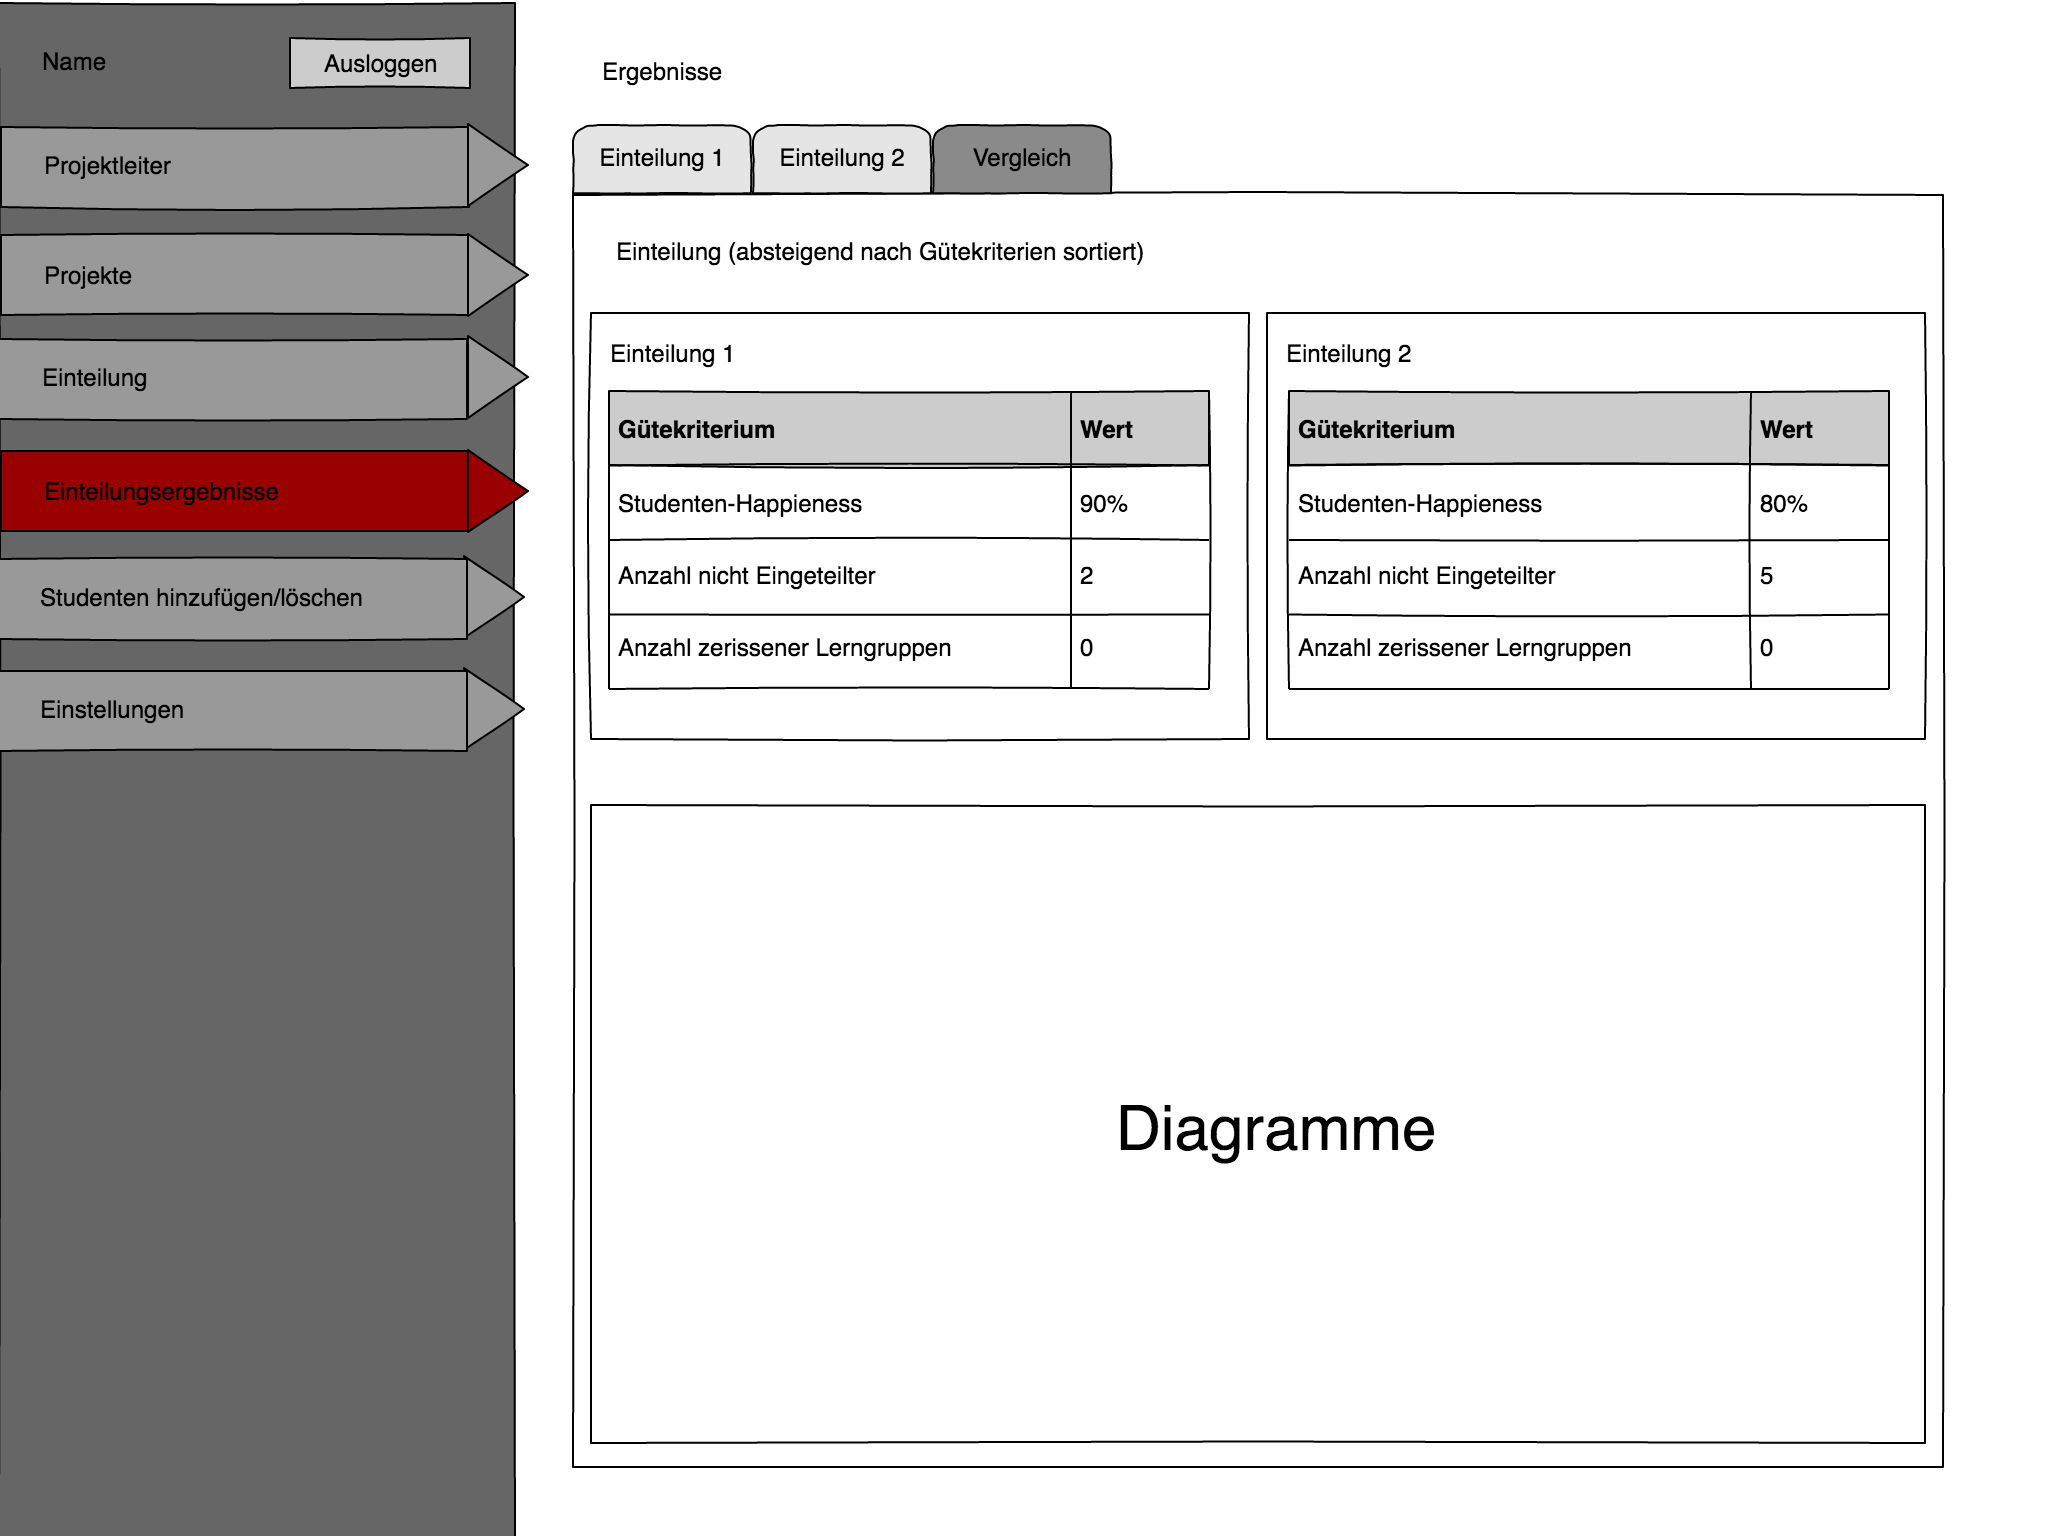
\includegraphics[width=\textwidth,
keepaspectratio=true]{gui/adminergebnissevergl.png}}
\captionof{figure}{Vergleichsansicht} \label{GUIvergleich}
\medskip
\fbox{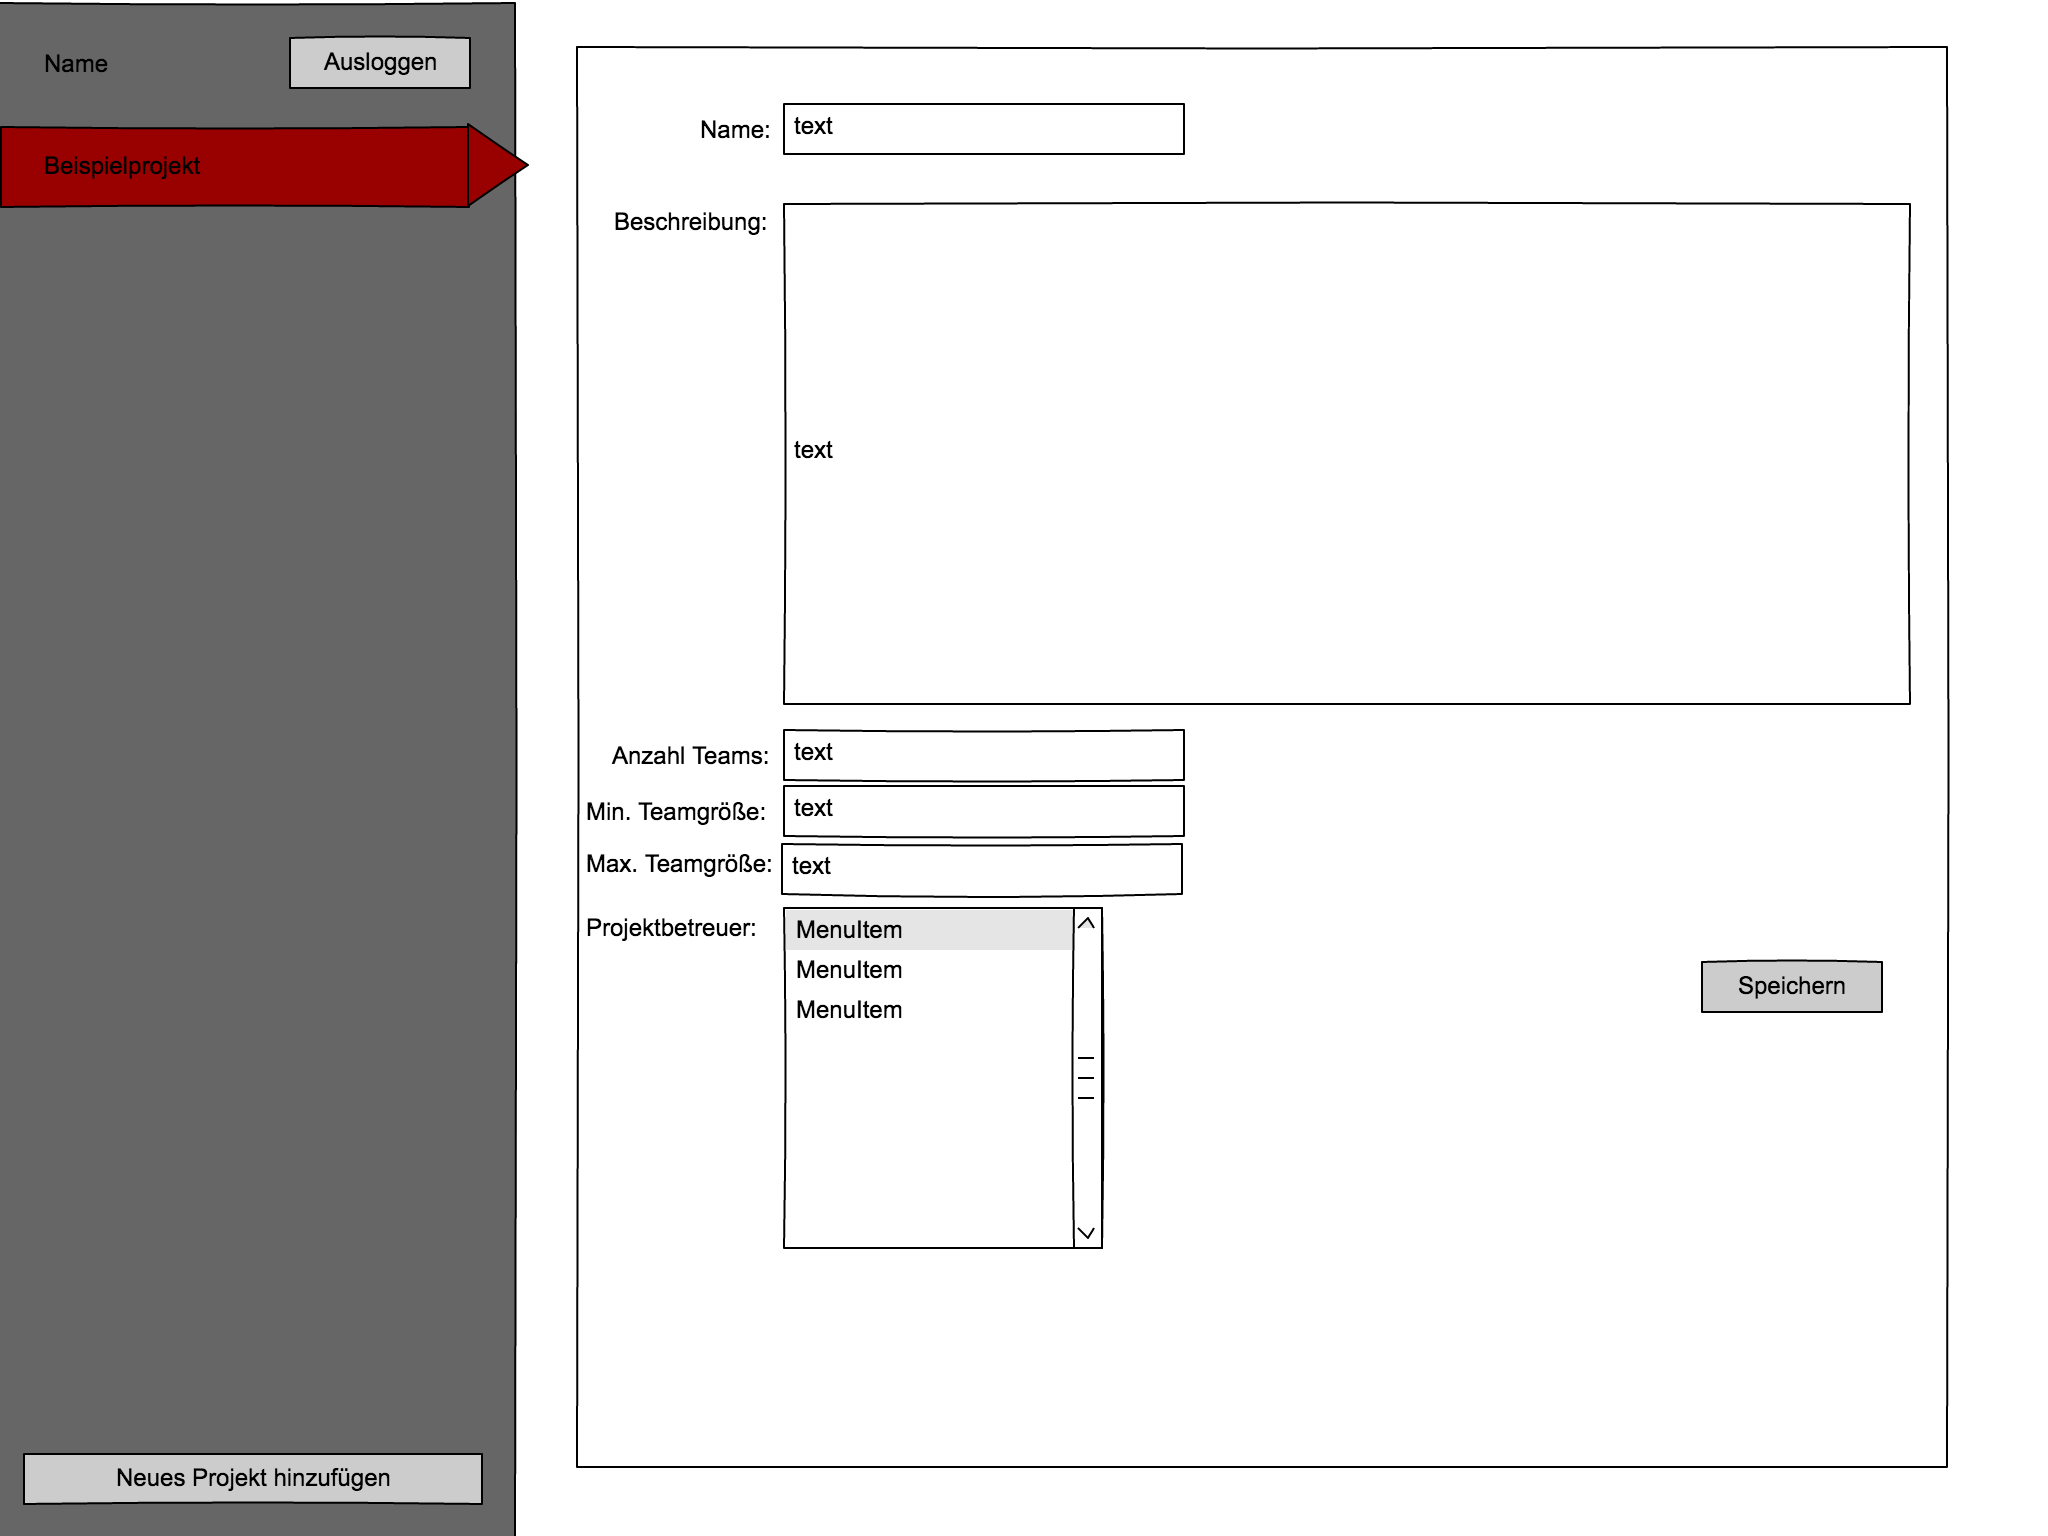
\includegraphics[width=\textwidth,
keepaspectratio=true]{gui/projleiterprojekte.png}}
\captionof{figure}{Betreueransicht} \label{GUIprojLeiterTeam}
\medskip
\fbox{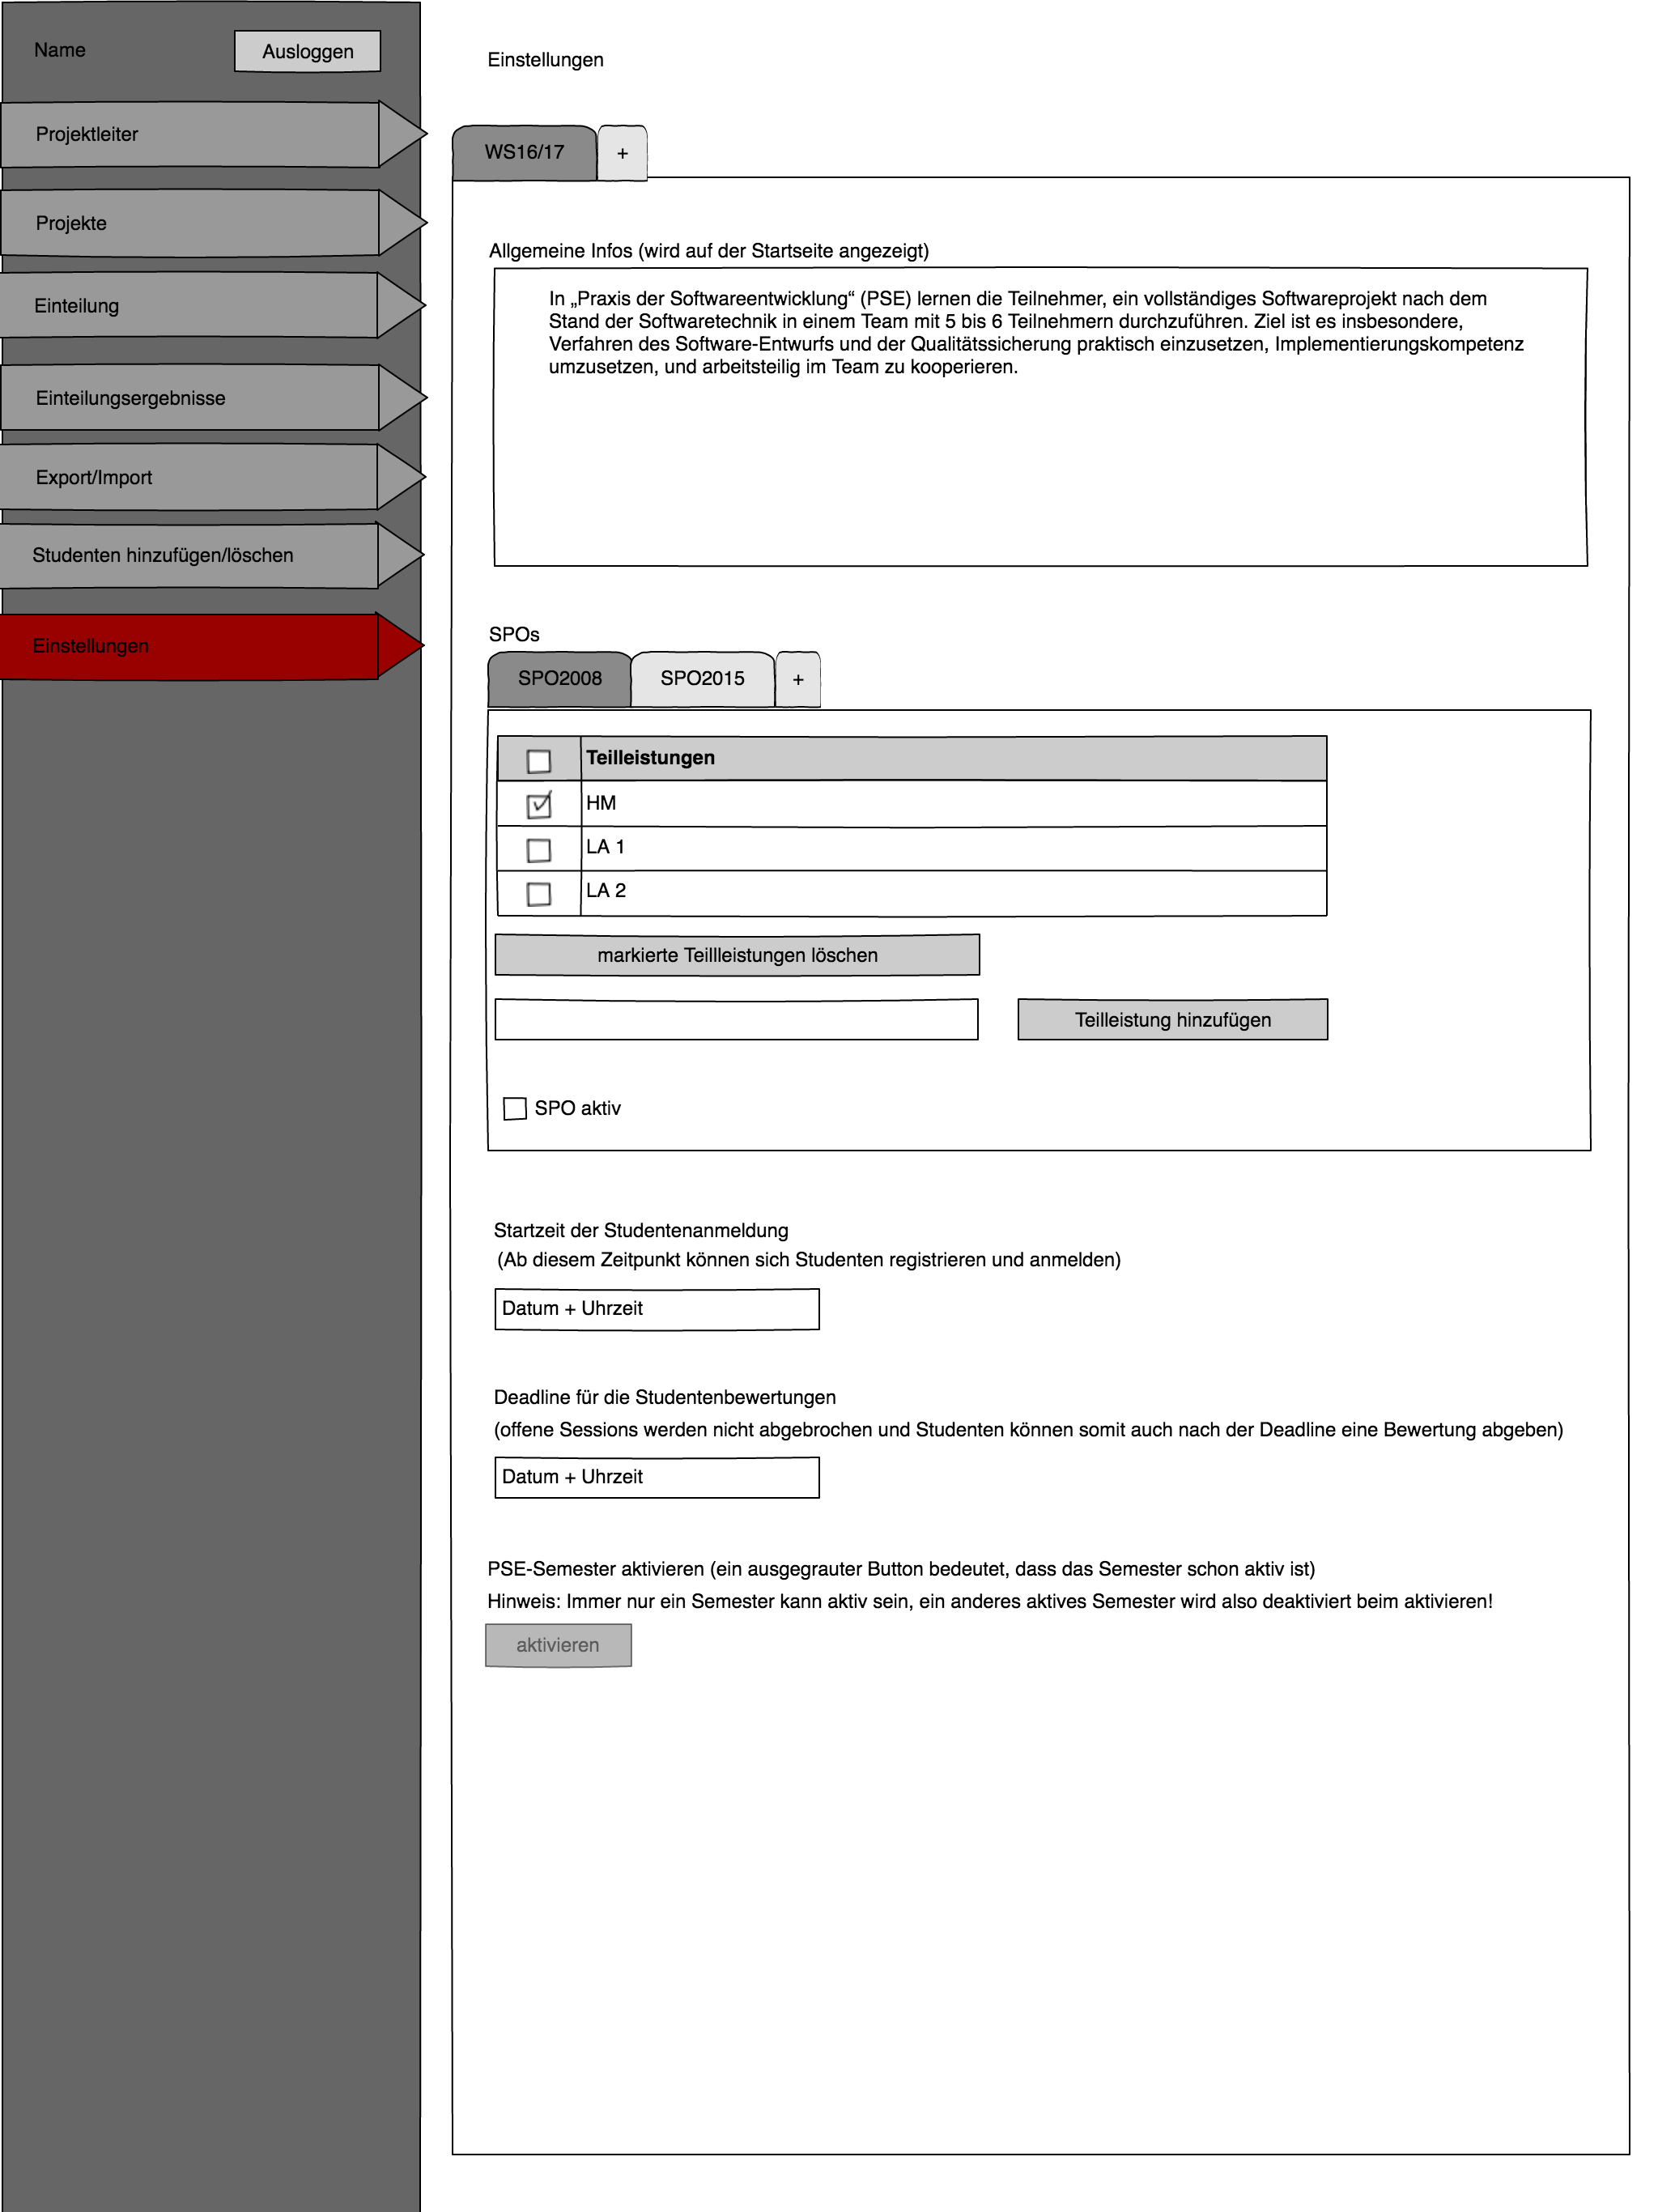
\includegraphics[width=\textwidth,
keepaspectratio=true]{gui/adminproperties.png}}
\captionof{figure}{Einstellungen} \label{GUIeinstellungen}
\medskip

}
%TODO LIZENZ
\end{enumerate}
\pagebreak
\printglossaries
\end{document}
